% STOP - Bitte zuerst lesen, bevor Sie weitermachen
%
% Einige Dinge müssen Sie an Ihre Bedürfnisse (und die Vorgaben Ihres
% Betreuers anpassen. Editieren Sie dazu die Datei docinfo.tex).
%
% 1. Sprache
% Das Template unterstützt Deutsch und Englisch, Standard ist Deutsch.
% Wenn Sie Englisch verwenden wollen, ändern Sie bitte direkt am Anfang
% dieser Datei den Eintrag
%    \newcommand{\hsmasprache}{de}
% auf
%    \newcommand{\hsmasprache}{en}
%
% 2. Form der Abgabe
% Das Template unterstützt sowohl eine digitale Abgabe, als auch eine Abgabe
% auf Papier. Bei einer Papierabgabe wird ein doppelseitiger Druck vorbereitet
% und der Titel wird so platziert, dass er in das Fenster des offiziellen
% Umschlages der Technischen Hochschule passt.
% Bei einer digitalen Abgabe (als PDF) wird der Titel zentriert und als
% Format wird einseitig gewählt. Außerdem wird die Datei unterschrift.png
% auf dem Blatt mit der Erklärung zur Eigenständigkeit eingebunden.
%
% 3. Zitierstil
% Abhängig von dem gewünschten Zitierstil passen Sie bitte in
% hma.cls die Einstellungen bei \RequirePackage[backend=biber...
% an. Wie ist dort genau erklärt.
% Achtung: Wenn Sie als Zitierstil Fußnoten wählen bzw. generell
% -------  mit Fußnoten arbeiten, dann beachten Sie bitte, dass
%          Fußnoten in Bildunterschriften und Tabellenüberschriften
%          nicht funktionieren.
%          Siehe hierzu https://texfaq.org/FAQ-ftncapt
%          und https://texfaq.org/FAQ-footintab
%          Sinnvollerweise verzichten Sie auf Fußnoten an diesen
%          Stellen und fügen Quellen einfach per \parancite ein.
%
% 4. Doppelseitiger oder einseitiger Druck
% Das Template bestimmt, ob einseitig oder doppelseitig gedruckt wird
% anhand der Abgabeform (papier / digital). Wollen sie dies übersteuern,
% müssen Sie in der Datei preambel.tex folgende Zeile
% \KOMAoptions{twoside=true} für doppelsetigen Druck
% \KOMAoptions{twoside=false} für einsetigen Druck
% direkt vor \usepackage{xcolor} einsetzen. Prinzipiell sollten Sie aber
% das vorgeschlagene Format einfach so lassen.
%
% 5. Unnötige Teile entfernen
% Entfernen Sie die Teile, die Sie nicht brauchen, z.B. Anhänge
%
% 6. Silbentrennung
% LaTeX führt eine automatische Silbentrennung durch. Allerdings
% werden Wörter, die bereits einen Bindestrich enthalten nicht
% getrennt, z.B. Datenschutz-Grundverordnung. Wenn Sie Ihren Text auf
% Deutsch schreiben, können Sie dann alternativ "= für den Bindestrich
% im Wort verwenden, z.B. Datenschutz"=Grundverordnung, damit LaTeX
% weiterhin richtig trennt.
% Ist die Silbentrennung aus einem anderen Grund nicht erfolgt, sodass
% das Wort über den rechten Rand hinaussteht oder wenn Sie eine weitere
% Trennstelle wollen, können Sie LaTeX helfen, indem Sie weitere
% Trennstellen angeben. Dies geschieht durch "- als Zeichen, z.B.
% Staats"-vertrag.
%
% 7. Nummerierung der Fußnoten
% LaTeX beginnt die Nummerierung der Fußnoten in jedem Kapitel wieder
% bei 1. In diesem Template wird die fortlaufende Nummerierung der Fußnoten 
% über die gesamte Arbeit umgesetzt.  
%
% 8. Unterschrift
% Bei einer Abgabe auf Papier unterschreiben Sie die Arbeit eigenhändig.
% Geben Sie allerdings digital ab, sollten Sie die Datei unterschrift.png in dem 
% Ordner /bilder durch einen Scan Ihrer eigenen Unteschrift ersetzen - andernfalls
% unterschreiben Sie als Max Mustermann ;-)
% *******************************************************************


% Dokumenteneinstellungen und Infos importieren
% -------------------------------------------------------
% Informationen und Einstellungen für Ihre Abschlussarbeit
%

% Sprache für das Dokument festlegen
\newcommand{\hsmasprache}{de} %de für Deutsch oder en für Englisch


% Abgabeform festlegen
% Bei einer digitalen Abgabe, wird das Dokument einseitig erzeugt und der Titel wird
% zentriert.
\newcommand{\hsmaabgabe}{digital} % Abgabe erfolgt für Fakultät I digital. Optionen hier sind für anderen Fakultäten: "papier" oder "digital".


% Flags für Veröffentlichung, Sperrvermerk
\newcommand{\hsmapublizieren}{opensource}   
% Wird einer Veröffentlichung zugestimmt?
% Optionen: 
% opensource = Druck der CC Lizenz mit By SA (Standard)
% hs = Veröffentlichung an der Technischen Hochschule und auf Hochschulservern
% stud = kein opensource und keine veröffentlichung auf den Hochschulservern
% vertraulich = Arbeit darf nicht veröffentlicht werden und erhält einen Sperrvermerk (Nur nach Absprache mit Betreuer setzen!)


\newcommand{\genderhinweis}{gender}     % Soll der Gender-Hinweis angezeigt werden? ja=gender, nein = nogender; Genderhinweis wird nur in deutscher Sprache angezeigt!


\newcommand{\hsmaquellcode}{sourcecode} % Verwenden Sie Quellcode in Ihrer Arbeit? ja=sourcecode, nein= nosourcecode

\newcommand{\hsmasymbole}{symbole} % Verwenden Sie viele Symbole in Ihrer Arbeit, welche in einem Symbolverzeichnis aufgeführt werden sollen? ja=symbole, nein= nosymbole


\newcommand{\hsmaglossar}{glossar} % Verwenden Sie Begriffserklärungen nicht Abkürzungen in Ihrer Arbeit? ja=glossar, nein= noglossar

\newcommand{\hsmatc}{tc} % Verwenden der Änderungsmarkierung. Änderungsmarkierung aktiv und eine Liste der Änderungen wird angezeigt = tc, Keine Änderungsmarkierung und keine Ausgabe der Änderungen = notc




% Titel der Arbeit auf Deutsch
\newcommand{\hsmatitelde}{Copyright-Scanner: Automatisierte Erkennung und Extraktion von Copyright-Vermerken mittels Large Language Models. Konzeption, prototypische Implementierung und Evaluation eines Al-gestützten Analysetools im Lizenz-Compliance-Kontext.}
\newcommand{\hsmatiteldeabstract}{Copyright-Scanner: Automatisierte Erkennung und Extraktion von Copyright-Vermerken mittels Large Language Models. Konzeption, prototypische Implementierung und Evaluation eines Al-gestützten Analysetools im Lizenz-Compli- ance-Kontext.}

% Titel der Arbeit auf Englisch
\newcommand{\hsmatitelen}{Copyright Scanner: Automated Detection and Extraction of Copyright Notices Using Large Language Models. Design, Prototype Implementation, and Evaluation of an AI-Based Analysis Tool in the Context of License Compliance.}

% Weitere Informationen zur Arbeit
\newcommand{\hsmaort}{Mannheim}          % Ort
\newcommand{\hsmaautorvname}{Romeo Aljoscha Eren}        % Vorname(n)
\newcommand{\hsmaautornname}{Türemis} % Nachname(n)
\newcommand{\hsmaabgabedatum}{2025-08-31}% Datum der Abgabe in dem Format JJJJ-MM-TT

\newcommand{\hsmafirma}{Metaeffekt GmbH, Heidelberg} % Firma bei der die Arbeit durchgeführt wurde
\newcommand{\hsmabetreuer}{Prof. Dr. Sven-Gunnar Klaus, Technische Hochschule Mannheim} % Betreuer an der Hochschule
\newcommand{\hsmazweitkorrektor}{Karsten Klein, metaeffekt GmbH}   % Betreuer im Unternehmen oder Zweitkorrektor

\newcommand{\hsmafakultaet}{I}    % I für Informatik oder E, S, B, D, M, N, W, V
\newcommand{\hsmastudiengang}{IB} % IB IMB UIB CSB IM MTB (weitere siehe titleblatt.tex)


% Preambel importieren
% Dokumententyp, benutzte Pakete und deren Einstellungen
\documentclass[	\hsmasprache,%
				\hsmaabgabe,%
				\hsmapublizieren,%
				\genderhinweis,
				\hsmaquellcode,
				\hsmasymbole,
				\hsmaglossar,
				\hsmatc]{HMA}

% Wo sind die Bilder?
\graphicspath{{bilder/}}


% Wo liegt Sourcecode?
\newcommand{\srcloc}{src/}


% Checklisten mit zwei Ebenen
\newlist{checklist}{itemize}{2}
\setlist[checklist]{label=$\square$}



% Befehl zum Erstellen eigener Makros. In diesem Fall ist es ein Makro für das Einbinden von Bildern. Das label (für \ref) ist dann der Name der Bilddatei
\newcommand{\bild}[3]{
	\begin{figure}[ht]
		\centering
		\includegraphics[width=#2]{#1}
		\caption{#3}
		\label{#1}
\end{figure}}




							


\newcommand{\snowcard}[9]{
	\begin{table}[ht!]
		\caption{\hsmasnowcardanforderung\ #1 -- #4}\label{#1}
		\renewcommand{\arraystretch}{1.2}
		\centering
		\sffamily
		\begin{footnotesize}

			\begin{tabularx}{\linewidth}{sssssl}
				\toprule
				\textbf{\hsmasnowcardno} & #1 & \textbf{\hsmasnowcardart} & #2 & \textbf{\hsmasnowcardprio} & #3 \\
				\midrule
				\multicolumn{2}{l}{\textbf{\hsmasnowcardtitel}} & \multicolumn{4}{l}{\parbox[t]{11.8cm}{#4}} \\
				\ifx&#5&%
				\else
				\multicolumn{2}{l}{\textbf{\hsmasnowcardherkunft}} & \multicolumn{4}{l}{\parbox[t]{11.8cm}{#5}} \\
				\fi
				\ifx&#6&%
				\else
				\multicolumn{2}{l}{\textbf{\hsmasnowcardkonflikt}} & \multicolumn{4}{l}{\parbox[t]{11.8cm}{#6}} \\
				\fi
				\addlinespace
				\multicolumn{6}{l}{\textbf{\hsmasnowcardbeschreibung}} \\
				\multicolumn{6}{l}{\parbox[t]{13.5cm}{#7\strut}} \\
				\ifx&#8&%
				\else
				\addlinespace
				\multicolumn{6}{l}{\textbf{\hsmasnowcardfitkriterium}} \\
				\multicolumn{6}{l}{\parbox[t]{13.5cm}{#8\strut}} \\
				\fi
				\ifx&#9&%

				\else
				\addlinespace
				\multicolumn{6}{l}{\textbf{\hsmasnowcardmaterial}} \\
				\multicolumn{6}{l}{\parbox[t]{13.5cm}{#9\strut}} \\
				\fi
				\bottomrule
			\end{tabularx}
		\end{footnotesize}
	\end{table}
}



% Quality Attribute Scenario
\newcommand{\qas}[9]{
	\begin{table}[ht!]
		\caption{\hsmaqasanforderung\ #1 -- #3}\label{#1}
		\renewcommand{\arraystretch}{1.2}
		\centering
		\sffamily
		\begin{footnotesize}

			\begin{tabularx}{\linewidth}{sssssl}
				\toprule
				\textbf{\hsmaqasno} & #1 & \textbf{\hsmaqasart} & QAS & \textbf{\hsmaqasprio} & #2 \\
				\midrule
				\multicolumn{2}{l}{\textbf{\hsmaqastitel}} & \multicolumn{4}{l}{\parbox[t]{11.8cm}{#3}} \\
				\multicolumn{2}{l}{\textbf{\hsmaqasquelle}} & \multicolumn{4}{l}{\parbox[t]{11.8cm}{#4}} \\
				\multicolumn{2}{l}{\textbf{\hsmaqasstimulus}} & \multicolumn{4}{l}{\parbox[t]{11.8cm}{#5}} \\
				\multicolumn{2}{l}{\textbf{\hsmaqasartefakt}} & \multicolumn{4}{l}{\parbox[t]{11.8cm}{#6}} \\
				\addlinespace
				\multicolumn{6}{l}{\textbf{\hsmaqasumgebung}} \\
				\multicolumn{6}{l}{\parbox[t]{13.5cm}{#7\strut}} \\
				\addlinespace
				\multicolumn{6}{l}{\textbf{\hsmaqasantwort}} \\
				\multicolumn{6}{l}{\parbox[t]{13.5cm}{#8\strut}} \\
				\addlinespace
				\multicolumn{6}{l}{\textbf{\hsmaqasmass}} \\
				\multicolumn{6}{l}{\parbox[t]{13.5cm}{#9\strut}} \\
				\bottomrule
			\end{tabularx}
		\end{footnotesize}
	\end{table}
}




%Abstrakt Ihrer Abschlussarbeit
% -------------------------------------------------------
% Abstrakt / Abstract
% Achtung: Wenn Sie im Abstrakt Anführungszeichen verwenden wollen, dann benutzen Sie
%          nicht "` und "', sondern \enquote{}. "` und "' werden nicht richtig
%          erkannt.

% Kurze (maximal halbseitige) Beschreibung, worum es in der Arbeit geht auf Deutsch
\newcommand{\hsmaabstractde}{Jemand musste Josef K. verleumdet haben, denn ohne dass er etwas Böses getan hätte, wurde er eines Morgens verhaftet. Wie ein Hund! sagte er, es war, als sollte die Scham ihn überleben. Als Gregor Samsa eines Morgens aus unruhigen Träumen erwachte, fand er sich in seinem Bett zu einem ungeheueren Ungeziefer verwandelt. Und es war ihnen wie eine Bestätigung ihrer neuen Träume und guten Absichten, als am Ziele ihrer Fahrt die Tochter als erste sich erhob und ihren jungen Körper dehnte. Es ist ein eigentümlicher Apparat, sagte der Offizier zu dem Forschungsreisenden und überblickte mit einem gewissermaßen bewundernden Blick den ihm doch wohl bekannten Apparat. Sie hätten noch ins Boot springen können, aber der Reisende hob ein schweres, geknotetes Tau vom Boden, drohte ihnen damit und hielt sie dadurch von dem Sprunge ab. In den letzten Jahrzehnten ist das Interesse an Künstlern sehr zurückgegangen. Aber sie überwanden sich, umdrängten den Käfig und wollten sich gar nicht fortrühren.}

% Kurze (maximal halbseitige) Beschreibung, worum es in der Arbeit geht auf Englisch
\newcommand{\hsmaabstracten}{The European languages are members of the same family. Their separate existence is a myth. For science, music, sport, etc, Europe uses the same vocabulary. The languages only differ in their grammar, their pronunciation and their most common words. Everyone realizes why a new common language would be desirable: one could refuse to pay expensive translators. To achieve this, it would be necessary to have uniform grammar, pronunciation and more common words. If several languages coalesce, the grammar of the resulting language is more simple and regular than that of the individual languages. The new common language will be more simple and regular than the existing European languages. It will be as simple as Occidental; in fact, it will be Occidental. To an English person, it will seem like simplified English, as a skeptical Cambridge friend of mine told me what Occidental is.}



% Literatur-Datenbank
\addbibresource{literatur.bib}   % BibLaTeX-Datei mit Literaturquellen einbinden


% Anfang des Dokuments
\begin{document}	


%Laden der Dateien mit Abkürzungen, Begriffserklärungen (Glossar), Symbole
% General
\newacronym{sca}{SCA}{Software Composition Analysis}
\newacronym{nlp}{NLP}{Natural Language Processing}
\newacronym{cli}{CLI}{Command Line Interface}
\newacronym{json}{JSON}{JavaScript Object Notation}
\newacronym{api}{API}{Application Programming Interface}
\newacronym{oss}{OSS}{Open Source Software}
\newacronym{urhg}{UrhG}{Urheberrechtsgesetz}
\newacronym{gpl}{GPL}{GNU General Public License}
\newacronym{wua}{WUA}{Welturheberrechtsabkommen}
\newacronym{rbü}{RBÜ}{Revidierte Berner Übereinkunft}

% Policy
\newacronym{cir}{CIR}{Copyright Identification Rule}
\newacronym{air}{AIR}{Author Identification Rule}
\newacronym{hir}{HIR}{Holder Identification Rule}
\newacronym[plural=CEPs, longplural=Copyright Extraction Policies]{cep}{CEP}{Copyright Extraction Policy}
\newacronym[plural=AEPs, longplural=Author Extraction Policies]{aep}{AEP}{Author Extraction Policy}
\newacronym[plural=HEPs, longplural=Holder Extraction Policies]{hep}{HEP}{Holder Extraction Policy}
\newacronym[plural=GEPs, longplural=General Extraction Policies]{gep}{GEP}{General Extraction Policy}

% LLMs
\newacronym[plural=LLMs, longplural=Large Language Models]{llm}{LLM}{Large Language Model}
\newacronym{ner}{NER}{Named Entity Recognition}
\newacronym{ie}{IE}{Information Extraction}
\newacronym{tp}{TP}{True Positive}
\newacronym{fp}{FP}{False Positive}
\newacronym{fn}{FN}{False Negative}

% metaeffekt
\newacronym{tmd}{TMD}{Terms Metadata}
% Glossareinträge
\newglossaryentry{glos:quantization}{name={Quantization}, description={beschreibt den Vorgang, bei dem die Genauigkeit von Modellgewichten reduziert wird, um das Modell kleiner und effizienter zu machen.}}
\newglossaryentry{glos:benchmark}{name={Benchmark}, description={ist ein standardisierter Test oder Vergleichswert, mit dem die Leistung, Qualität oder Effizienz von Systemen, Prozessen oder Produkten objektiv bewertet wird.}}
\newglossaryentry{glos:fine-tuning}{name={Fine-Tuning}, description={ist der Prozess, bei dem ein bereits vortrainiertes Modell mit zusätzlichen, spezifischen Daten nachtrainiert wird, um es besser auf bestimmte Aufgaben oder Anwendungsbereiche abzustimmen.}}


%% Verzeichnis von Symbolen und Einheiten
\newglossaryentry{symb:Pi}{name=\ensuremath{\pi},
	description={Geometrical value},
	unit={},
	type=symbolslist}

\newglossaryentry{symb:energyconsump}{name=\ensuremath{P},
	description={Energy consumption},
	unit={\si{kW}},
	type=symbolslist}

	
\pagestyle{headings}
\tableofcontents


\mainmatter

%% Ihre Inhaltsdateien werden an dieser Stelle in das Dokument eingefügt
\chapter{Einleitung}\label{ch:einleitung}

\glspl{llm} stehen zunehmend im Zentrum hitziger Debatten über Urheberrechtsverletzungen.
Ihre Fähigkeit, menschenähnliche Texte zu generieren, basiert auf dem Training mit riesigen Datenmengen aus dem Internet, deren Verwendung rechtlich und ethisch zunehmend infrage gestellt wird.
Inmitten dieser Diskussion, in der \glspl{llm} oft als potenzielle Rechtsverletzer dargestellt werden, bleibt die Möglichkeit weitgehend unbeachtet, ebenjene Technologie nicht zur Umgehung, sondern zur Wahrung des Urheberrechts einzusetzen.
Tatsächlich verfügen \glspl{llm} über ein bemerkenswertes Potenzial, die komplexen und oft unstrukturierten Informationen in Softwareprojekten zu verstehen.
Ihre Fähigkeit, kontextuelle Zusammenhänge zu erkennen und semantische Feinheiten zu interpretieren, eröffnet neue Wege für die automatisierte Analyse.
Diese Fähigkeiten sind umso relevanter, als die Einhaltung von Lizenzbestimmungen in modernen Software-Lieferketten immer komplexer wird und traditionelle, regelbasierte Systeme an ihre Grenzen stoßen.

% ======================================================================================================================

\section{Einführung in die Relevanz des License Compliance Managements und die Rolle von Copyright-Statements}\label{sec:einfuhrung}

In der modernen Softwareentwicklung ist die Einhaltung von Lizenzbedingungen, bekannt als License Compliance Management, von zentraler Bedeutung.
Denn Softwareprodukte sind heute selten monolithische Eigenentwicklungen, sondern komplexe Systeme, die aus einer Vielzahl von Drittanbieter- und Open-Source-Komponenten bestehen.
Jede dieser Komponenten unterliegt spezifischen Lizenzverträgen, die neben Bedingungen und Einschränkung insbesondere Verpflichtungen, etwa die Nennung des Urhebers oder die Beibehaltung von Lizenztexten, vorschreiben.
Die systematische Erfassung und Dokumentation dieser Abhängigkeiten ist unerlässlich, um rechtliche Risiken wie Urheberrechtsverletzungen zu minimieren und die Konformität über die gesamte Software-Lieferkette sicherzustellen.

Ein zentrales Instrument zur Gewährleistung dieser Konformität ist der sogenannte Software-Annex, ein von der metaeffekt GmbH für ihre Kunden erstelltes Begleitdokument.
Es dient als transparente und nachvollziehbare Bestandsliste (Bill of Materials), die, wie in Abbildung~\ref{fig:annex-01} exemplarisch gezeigt, alle Software-Bestandteile systematisch erfasst.
Die Abbildung verdeutlicht wie physische Dateien, sogenannte Artefakte wie beispielsweise \texttt{log4j-core-2.14.0.jar}, zu logischen Einheiten, den Komponenten (z.B. \enquote{Apache Log4j}), zusammengefasst werden.
Dieser Ansatz ermöglicht eine klare Zuordnung der geltenden Lizenzen auf Komponentenebene.
Durch diese strukturierte Aufstellung bündelt der Annex alle zur Erfüllung der Lizenzpflichten notwendigen Informationen und umfasst darüber hinaus eine Sammlung der relevanten Lizenztexte sowie eventuell geforderte Lizenzhinweise.

\begin{figure}[ht]
    \centering
    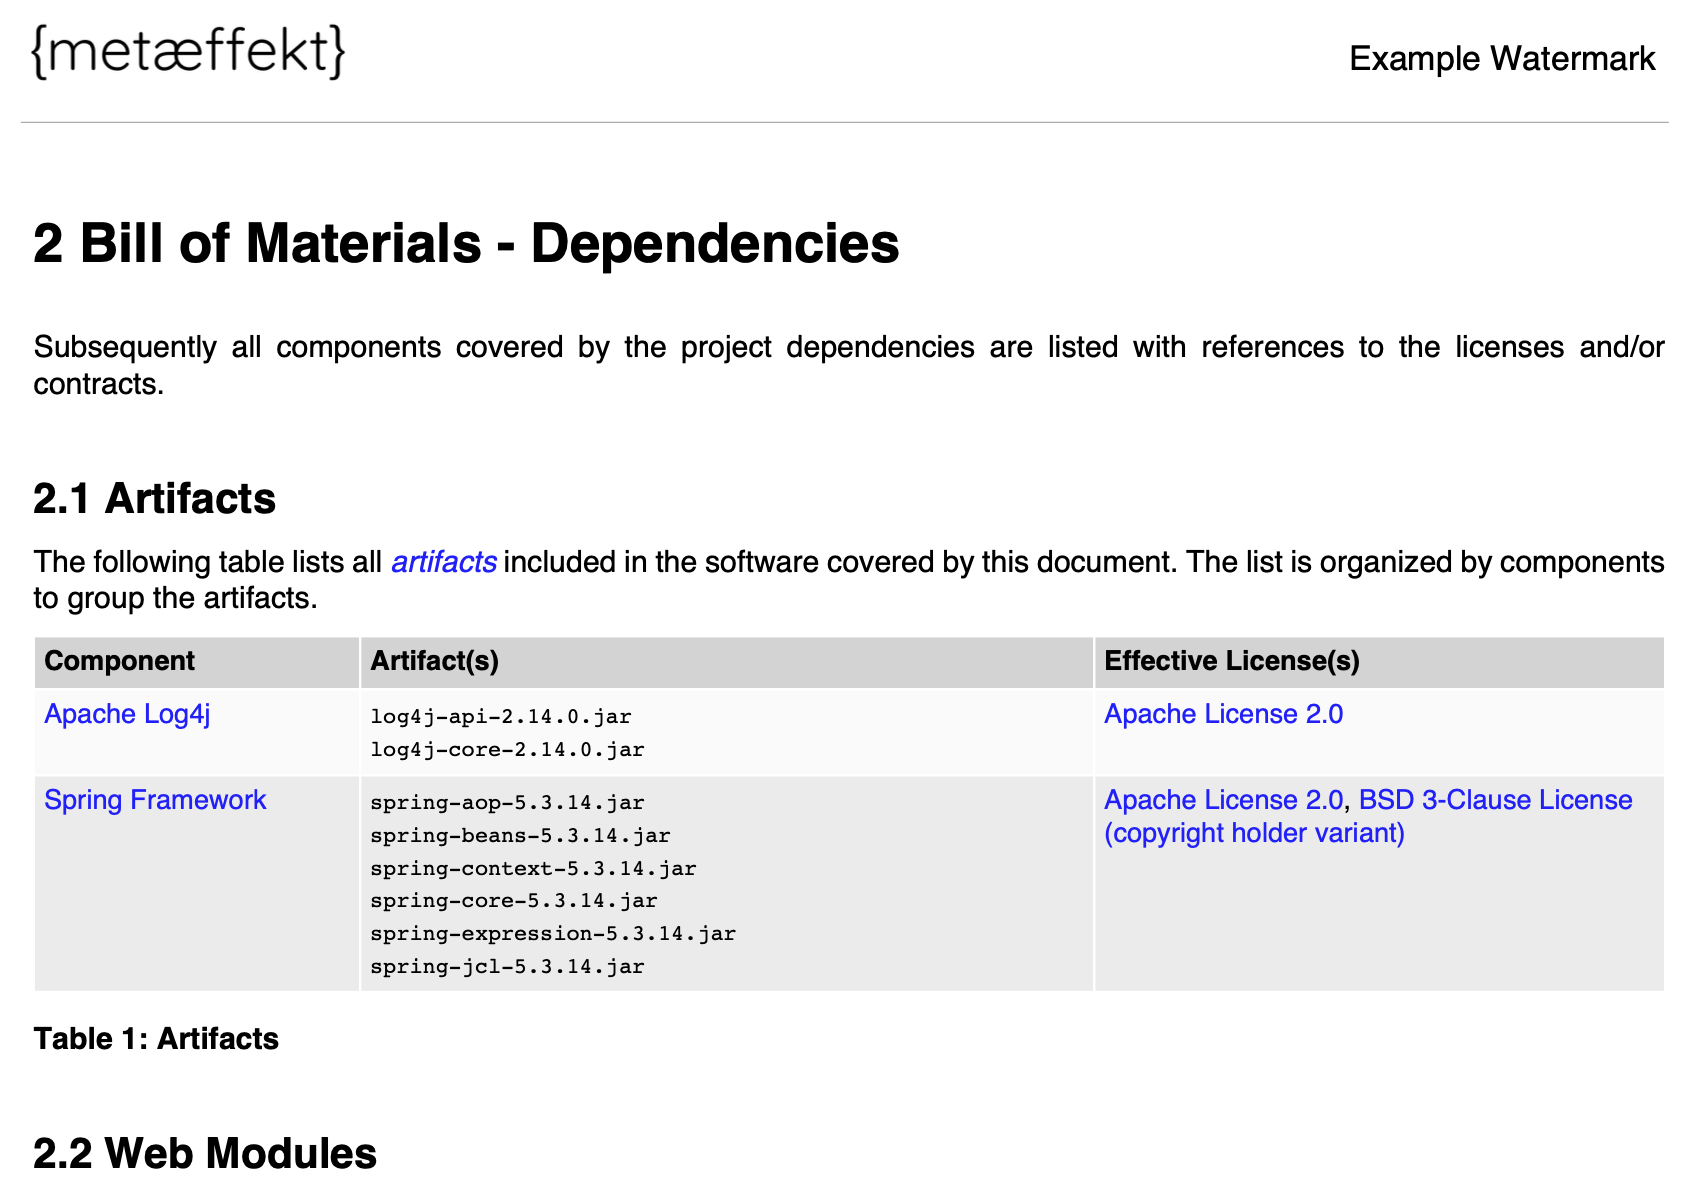
\includegraphics[width=\textwidth]{einleitung/screenshot-annex-01.png}
    \caption{Ausschnitt aus einem beispielhaften Software-Annex, der die tabellarische Aufstellung der Software-Komponenten (Component), der zugehörigen Artefakte (Artifacts) und der für sie geltenden Lizenzen (Effective Licenses) zeigt. Diese detaillierte Zuordnung ist die Grundlage für die rechtssichere Auslieferung von Software.}
    \label{fig:annex-01}
\end{figure}

Den im Annex dokumentierten Copyright-Statements kommt ebenfalls eine wesentliche Bedeutung zu.
Ihre korrekte und unveränderte Wiedergabe ist in vielen Fällen Teil der rechtlichen Verpflichtungen, die sich aus den jeweiligen Lizenzen ergeben.
Abbildung~\ref{fig:annex-02} illustriert diesen Sachverhalt am Beispiel der Komponente \textit{Spring Framework}.
Dort wird explizit aufgeführt, dass die BSD 3-Clause Lizenz die Reproduktion des spezifischen Copyright-Vermerks \enquote{Copyright (c) 2000-2011 INRIA, France Telecom All rights reserved.} erfordert.
Die Extraktion solcher Vermerke ist daher keine technische Formalität, sondern eine Notwendigkeit zur Lizenzerfüllung.
Die Vollständigkeit und Fehlerfreiheit dieser Informationen wirkt sich somit direkt auf die Rechtskonformität des gesamten Softwareprodukts aus.
Die automatisierte und präzise Identifikation dieser Statements ist eine Voraussetzung für ein effektives und skalierbares License Compliance Management.

\begin{figure}[ht]
    \centering
    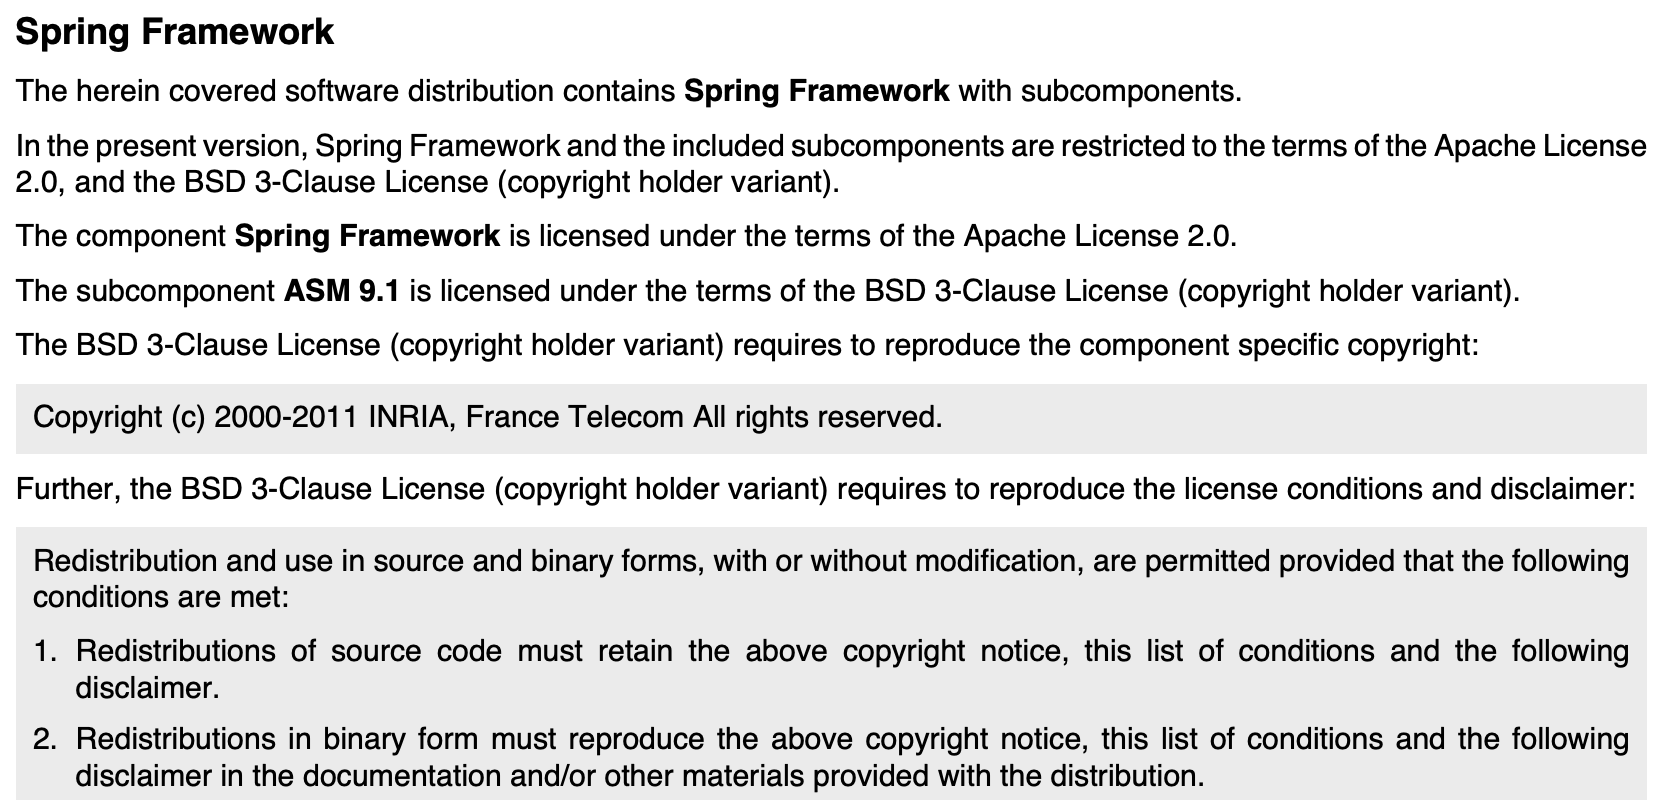
\includegraphics[width=\textwidth]{einleitung/screenshot-annex-02.png}
    \caption{Beispielhafter Auszug aus dem Abschnitt \textit{License Notices} eines Annex. Es wird gezeigt, wie für die Komponente \textit{Spring Framework} eine konkrete Lizenzverpflichtung der BSD 3-Clause Lizenz erfüllt wird, indem der dazugehörige Copyright-Vermerk sowie die Lizenzbedingungen exakt reproduziert werden.}
    \label{fig:annex-02}
\end{figure}

% ======================================================================================================================

\section{Darstellung der Problemstellung bei der automatisierten Extraktion von Copyright-Informationen}\label{sec:problemstellung}

Die automatisierte Extraktion von Copyright-Informationen ist für die rechtssichere Nutzung von Software unerlässlich, doch die etablierten Werkzeuge stoßen in der Praxis an grundlegende methodische Grenzen.
Die größte Herausforderung besteht darin, dass urheberrechtliche Vermerke in Softwareprojekten keinem einheitlichen Standard folgen, sondern über Jahrzehnte in unzähligen Variationen und oft formlos direkt im Quellcode oder begleitenden Hinweisen eingebracht wurden.
Bestehende Analysesysteme setzen vorwiegend auf starre, regelbasierte Verfahren, die dieser Vielfalt nicht gerecht werden und die oft subtilen, kontextabhängigen Bedeutungen nicht erfassen können.

Diese technologische Limitierung führt zu mehreren Problemen.
Zum einen verändern die Werkzeuge häufig die extrahierten Copyright-Vermerke, indem sie beispielsweise Formatierungen oder die ursprüngliche Schreibweise anpassen.
Solche Eingriffe können jedoch die Integrität und die rechtliche Aussagekraft der Originalangabe verfälschen.
Zum anderen scheitern diese Systeme oft daran, zusammengehörige Blöcke mit mehreren Copyright-Angaben als eine Einheit zu erkennen, was zum Verlust des erforderlichen Kontextes führt.
Darüber hinaus ist die Erkennung aller beitragenden Autoren unzureichend, da viele Mitwirkende an Positionen im Quellcode genannt werden, die von einfachen Suchmustern nicht erfasst werden.

Das Kernproblem resultiert folglich aus der methodischen Diskrepanz zwischen deterministischen, regelbasierten Extraktionsansätzen und der heterogenen, semantisch vielfältigen Natur der zu analysierenden Daten.
Die daraus folgenden fehlerhaften und unvollständigen Extraktionen erfordern einen hohen manuellen Nachbesserungsaufwand und stellen ein fortwährendes Risiko für die Lizenz-Compliance dar.

% ======================================================================================================================

\section{Zielsetzung der Arbeit}\label{sec:zielsetzung}

Das zentrale Ziel dieser Arbeit ist die Entwicklung und Bewertung eines neuartigen, auf künstlicher Intelligenz basierenden Copyright-Scanners.
Dieser soll die methodischen Schwächen existierender, regelbasierter Systeme adressieren.
Die Untersuchung konzentriert sich darauf, wie \glspl{llm} genutzt werden können, um Copyright-Informationen präziser und im Einklang mit spezifischen Compliance-Richtlinien zu extrahieren.
Es wird ein Prototyp implementiert und evaluiert, um das Potenzial dieses Ansatzes für den praktischen Einsatz im Lizenzmanagement aufzuzeigen.

% ======================================================================================================================

\section{Abgrenzung des Projektumfangs und Erläuterung der methodischen Vorgehensweise}\label{sec:abgrenzung}

Diese Arbeit grenzt sich insofern von verwandten Forschungsfeldern ab, als dass sie nicht die Aufdeckung von Copyright-Verstößen zum Ziel hat.
Der Projektumfang konzentriert sich stattdessen vollständig auf die Entwicklung und Bewertung von Methoden zur präzisen Extraktion der urheberrechtlich relevanten Metadaten.
Die methodische Vorgehensweise ist mehrstufig aufgebaut und folgt einem iterativen Ansatz, bei dem die Erkenntnisse aus den einzelnen Phasen direkt in die kontinuierliche Verbesserung und Anpassung einer im Rahmen dieser Arbeit entwickelten \textit{Copyright Identification and Extraction Policy} (im weiteren Verlauf mit Policy bezeichnet) einfließen.

Zuerst erfolgt eine systematische Datenaggregation, um eine hochwertige Test- und Evaluationsgrundlage zu schaffen.
Darauf aufbauend wird ein umfassender Benchmark verschiedener Sprachmodelle durchgeführt, um ein geeignetes Basismodell zu identifizieren.
Im nächsten Schritt wird dessen Leistung durch gezieltes Prompt-Engineering iterativ verbessert.
Abschließend wird mittels Fine-Tuning untersucht, ob ein spezialisiertes, kleineres Modell eine vergleichbare Genauigkeit bei höherer Effizienz erreichen kann.
\chapter{Grundlagen}\label{ch:grundlagen}

% ======================================================================================================================

\section{Rechtliche Grundlagen}\label{sec:rechtliches}

Die zunehmende Verbreitung von \gls{oss} in Forschung, Wirtschaft und öffentlicher Verwaltung wirft eine Vielzahl rechtlicher Fragen auf, die sich insbesondere auf das Urheberrecht und die Lizenzierungspraxis beziehen.
Obwohl OSS häufig frei zugänglich ist, unterliegt sie in Deutschland uneingeschränkt dem Schutz des Urheberrechts gemäß dem \gls{urhg}\autocite{noauthor_urhg_nodate}.
Die rechtssichere Nutzung, Veränderung und Weiterverbreitung quelloffener Software setzt daher ein grundlegendes Verständnis der urheberrechtlichen Schutzmechanismen, der Einräumung und Durchsetzung von Nutzungsrechten sowie der Einhaltung von Lizenzbedingungen voraus.
Gerade im Kontext automatisierter Softwareanalysen, etwa durch \glspl{llm}, rücken Fragen der korrekten Attribution, der Wahrung von Lizenzpflichten und der Erkennbarkeit urheberrechtlicher Hinweise im Code in den Fokus.
Dieses Kapitel beleuchtet die rechtlichen Grundlagen für den Einsatz von \gls{oss}, analysiert spezifische Regelungen des deutschen \gls{urhg} im Bereich der Software, zeigt potenzielle Konflikte innerhalb der Software-Lieferkette und stellt die Konsequenzen urheberrechtlicher Verstöße systematisch dar.

% ----------------------------------------------------------------------------------------------------------------------

\subsection{Grundlagen des Urheberrechts}

Das deutsche \acrlong{urhg} schützt die geistigen Schöpfungen von Autoren, Künstlern und anderen Kreativen.
Ziel des Urheberrechts ist es, sowohl die persönlichen als auch die wirtschaftlichen Interessen des Urhebers zu sichern (§ 11 \gls{urhg}).
Die zentrale Voraussetzung für den Schutz ist die sogenannte Schöpfungshöhe, also ein gewisses Maß an Individualität des Werkes.
Ein urheberrechtlicher Schutz entsteht automatisch mit der Schaffung des Werkes, eine Registrierung ist nicht erforderlich.

Gemäß § 2 Absatz 1 \gls{urhg} gehören Computerprogramme ausdrücklich zu den schutzfähigen Werken.
Sie werden unter Punkt 1 als \enquote{Werke der Literatur} erfasst, unabhängig davon, ob sie künstlerisch anspruchsvoll oder lediglich funktional gestaltet sind.
Der Urheber im Sinne des \gls{urhg} ist die natürliche Person, die das Werk geschaffen hat (§ 7 \gls{urhg}).

Für das Verständnis von \gls{oss} ist besonders relevant, dass die Schutzwirkung des Urheberrechts unabhängig davon gilt, ob das Werk kommerziell oder unentgeltlich verwendet werden soll.
Auch öffentlich zugängliche Software unterliegt dem Urheberrecht, und ihre Nutzung bedarf grundsätzlich der Zustimmung des Rechteinhabers (§§ 15 ff. \gls{urhg}).

% ----------------------------------------------------------------------------------------------------------------------

\subsection{Computerprogramme als besondere Werkform (§§ 69a–69g \gls{urhg})}

Im Jahr 1993 wurden durch die §§ 69a bis 69g \gls{urhg} spezielle Regelungen für Computerprogramme in das Gesetz aufgenommen.
Diese Vorschriften basieren auf der EU-Richtlinie 2009/24/EG über den Rechtsschutz von Computerprogrammen.
Software gilt damit als eine eigenständige Werkform mit besonderen Regelungen, die sich in Teilen von den allgemeinen Bestimmungen des Urheberrechts unterscheiden.

Nach § 69a \gls{urhg} sind Programme geschützt, wenn sie eine persönliche geistige Schöpfung des Urhebers darstellen.
Der Schutz bezieht sich nicht nur auf den Quellcode, sondern auch auf vorbereitende Entwurfsunterlagen, sofern sie unmittelbar zur Entwicklung eines Programms bestimmt sind.

§ 69b \gls{urhg} bestimmt, dass der Urheber eines Programms in aller Regel diejenige Person ist, die es entwickelt hat.
Wird die Software jedoch im Rahmen eines Arbeitsverhältnisses erstellt, gehen die uneingeschränkten Nutzungsrechte grundsätzlich auf den Arbeitgeber über.

Die in § 69c \gls{urhg} genannten Rechte des Rechteinhabers umfassen unter anderem das dauerhafte oder vorübergehende Vervielfältigen, Übersetzen, Bearbeiten oder anderweitige Umarbeiten eines Programms sowie dessen öffentliche Wiedergabe.
§ 69d \gls{urhg} regelt die zulässigen Handlungen.
Beispielsweise darf ein rechtmäßiger Nutzer ein Programm vervielfältigen oder beobachten, wenn dies für dessen bestimmungsgemäße Nutzung erforderlich ist.

§ 69e \gls{urhg} erlaubt einem Nutzer unter bestimmten Voraussetzungen die Dekompilierung eines Programms.
Ziel dieser Regelung ist insbesondere die Sicherstellung der Interoperabilität mit anderen Programmen.
Gerade im Open-Source-Kontext kann diese Vorschrift bei der Analyse proprietärer Schnittstellen von Bedeutung sein.

% ----------------------------------------------------------------------------------------------------------------------

\subsection{Einräumung von Nutzungsrechten (§§ 31–33 \gls{urhg})}

Ein zentrales Instrument für die Verbreitung und Nutzung von Software ist die Einräumung von Nutzungsrechten.
Diese ist im Urheberrecht in den §§ 31 bis 33 \gls{urhg}geregelt.
Während das Urheberrecht als solches nicht übertragbar ist (§ 29 Abs. 1 \gls{urhg}), können Nutzungsrechte an einem Werk sehr wohl eingeräumt werden.
Hierbei wird zwischen einfachen und ausschließlichen Nutzungsrechten unterschieden (§ 31 Abs. 2 \gls{urhg}).
Einfache Nutzungsrechte erlauben die gleichzeitige Nutzung durch mehrere Personen, während ausschließliche Rechte eine exklusive Nutzung vorsehen.

Software Lizenzen allgemein und insbesondere Open-Source-Lizenzen wie die \gls{gpl}\footnote{\url{https://www.gnu.org/licenses/gpl-3.0.de.html}}, die MIT License\footnote{\url{https://opensource.org/license/mit}} oder die Apache
License\footnote{\url{https://www.apache.org/licenses/LICENSE-2.0}} gewähren typischerweise einfache Nutzungsrechte.
Diese standardisierten Lizenzverträge werden wirksam, sobald die Software verwendet oder öffentlich verfügbar gemacht wird.

§ 32 \gls{urhg} regelt die angemessene Vergütung des Urhebers.
Im Bereich von \gls{oss} kommt dieser Vorschrift meist keine praktische Bedeutung zu, da die Lizenzen oft ausdrücklich auf eine Vergütung verzichten.
Dennoch ist rechtlich klar, dass die Unentgeltlichkeit der Nutzung nicht automatisch bedeutet, dass der Urheber auf seine Rechte verzichtet.

§ 33 \gls{urhg} betrifft die Übertragbarkeit von Rechten.
Diese Vorschrift kann beispielsweise bei der Weitergabe von Projekten, dem Forking oder der Übernahme von \gls{oss}-Komponenten durch Dritte relevant sein.

Ein rechtlich entscheidender Punkt bei Software-Lizenzierung sind die damit verbundenen Verpflichtungen, insbesondere die sogenannten Copyleft-Klauseln, wie sie prominent in der \gls{gpl} zu finden sind.
Diese Klauseln verpflichten den Lizenznehmer, bei einer Weiterverbreitung des Werkes oder abgeleiteter Versionen davon, diese ebenfalls unter die Bedingungen der ursprünglichen Lizenz zu stellen.
Diese Verpflichtungen gelten als Bedingungen für die Einräumung der Nutzungsrechte.
Hält sich ein Nutzer nicht an diese Verpflichtungen, indem er beispielsweise den Quellcode einer veränderten GPL-Software nicht mitliefert, handelt er so, als hätte er nie eine Lizenz erhalten.
Die daraus resultierende Urheberrechtsverletzung wird im Abschnitt \ref{subsec:rechtsfolgen-bei-urheberrechtsverstoen} behandelt.
% TODO: Eventuell genauer auf Copyleft und Viralen-Effekt eingehen

% ----------------------------------------------------------------------------------------------------------------------

\subsection{Anwendung auf Open Source Software}

\gls{oss} unterliegt dem Urheberrecht oder ähnlichen internationalen Rechten unabhängig davon, ob sie frei oder kostenpflichtig zur Verfügung steht.
Der entscheidende Unterschied zu proprietärer Software besteht darin, dass die Rechteinhaber ihre Nutzungsrechte bewusst in standardisierten Lizenztexten öffentlich freigeben.
Diese Freigabe erfolgt meist in Form einfacher Nutzungsrechte im Sinne von § 31 Abs. 2 \gls{urhg}.

Einige Open-Source-Lizenzen, insbesondere solche mit sogenannten Copyleft-Klauseln wie die \gls{gpl}, verpflichten zur Offenlegung des modifizierten Quellcodes, sofern die Software weiterverbreitet wird.
Andere Lizenzen wie die MIT oder Apache License erlauben eine freiere Weiterverwendung, auch in proprietären Softwareprodukten.

Open Source kann somit entweder auf vertraglicher Grundlage oder, in bestimmten Fällen, durch gesetzliche Schranken genutzt werden.
Voraussetzung ist stets, dass die Nutzungsrechte ordnungsgemäß eingeräumt wurden.
Das Urheberrecht bleibt auch dann bestehen, wenn keine kommerziellen Interessen verfolgt werden.

% ----------------------------------------------------------------------------------------------------------------------

\subsection{Rechtsfolgen bei Urheberrechtsverstößen}\label{subsec:rechtsfolgen-bei-urheberrechtsverstoen}

Die Verletzung urheberrechtlicher Vorschriften oder die Nichtbeachtung von Lizenzbedingungen kann weitreichende rechtliche Folgen haben.
Nach § 97 \gls{urhg} hat der Urheber Anspruch auf Unterlassung und Beseitigung der Beeinträchtigung.
Darüber hinaus kann ein Anspruch auf Schadensersatz bestehen, der je nach Sachlage entweder auf dem konkreten Schaden, dem Gewinn des Verletzers oder einer fiktiven Lizenzgebühr basiert.

§ 98 \gls{urhg} ermöglicht es zudem, rechtswidrig hergestellte oder verbreitete Vervielfältigungsstücke zu vernichten oder vom Markt zu nehmen.
In besonders schweren Fällen sind sogar strafrechtliche Sanktionen nach § 106 \gls{urhg} möglich, etwa bei vorsätzlicher und gewerbsmäßiger Verletzung des Urheberrechts.
Wer \gls{oss} einsetzt oder weiterverbreitet, trägt daher die Verantwortung, die jeweiligen Lizenzbedingungen genau zu beachten.
Wird beispielsweise eine Lizenzbedingung der \gls{gpl} verletzt, etwa durch Nichtoffenlegung des Quellcodes, kann die Lizenzwirkung entfallen.
In diesem Fall ist jede weitere Nutzung als unrechtmäßige Verwertung zu bewerten, mit allen sich daraus ergebenden rechtlichen Konsequenzen.

% ----------------------------------------------------------------------------------------------------------------------

\subsection{Copyright-Vermerke und Autorenkennzeichen im Quellcode}

In der Open-Source-Softwareentwicklung ist es üblich, urheberrechtlich relevante Informationen direkt im Quellcode zu vermerken.
Dazu zählen Copyright-Hinweise, Autorenkennzeichen und Lizenzvermerke.
Diese Informationen dienen nicht der Entstehung des Urheberrechts, das automatisch mit der Schöpfung eines Werkes entsteht (§ 7 UrhG), erfüllen jedoch eine bedeutende Funktion.
Sie ermöglichen die Zurechnung von Urheberschaft, stellen sicher, dass Lizenzbedingungen bekannt gemacht werden, und unterstützen die Einhaltung der rechtlichen Rahmenbedingungen bei der Weitergabe.
Durch standardisierte Angaben wie SPDX-License-Identifier können solche Informationen zudem maschinell ausgelesen werden.

%Insbesondere bei der Nutzung von Large Language Models zur automatisierten Analyse von Software bieten diese Metadaten eine wichtige Grundlage.
%Durch Extraktion und semantische Analyse können solche Systeme helfen, Lizenzen korrekt zu erkennen, Urheber zu identifizieren und rechtliche Risiken bei der Weiterverwendung von Quellcode zu minimieren.

% ----------------------------------------------------------------------------------------------------------------------

\subsection{Auswirkungen auf die Software-Lieferkette}

Die zunehmende Verwendung von \gls{oss} in komplexen IT-Systemen führt dazu, dass Softwareprodukte häufig auf der Basis zahlreicher externer Komponenten aufgebaut werden.
Daraus ergeben sich rechtlich relevante Abhängigkeiten innerhalb der Software-Lieferkette.

Jede dieser Komponenten unterliegt bestimmten Nutzungsbedingungen, die über die jeweilige Lizenz definiert sind.
Werden diese Bedingungen nicht eingehalten, etwa durch Nichtbeachtung von Namensnennungspflichten oder durch unzulässige Integration in proprietäre Systeme, kann dies dazu führen, dass das Nutzungsrecht erlischt und eine Urheberrechtsverletzung vorliegt (§ 97 UrhG).

Für Unternehmen und Entwickler bedeutet dies, dass alle eingebundenen Komponenten erfasst, lizenziert und dokumentiert werden müssen.
Die Anforderungen an die Compliance steigen mit der Komplexität des Produkts.
%Hier können automatisierte Verfahren, etwa auf Basis von \glspl{llm}, eine große Unterstützung bieten, indem sie Lizenztexte analysieren, Copyright-Vermerke erkennen und auf potenzielle Verstöße hinweisen.

% ----------------------------------------------------------------------------------------------------------------------

\subsection{Internationale Urheberrechtsregelungen}

Die rechtliche Einbettung des Urheberrechts ist nicht allein national geregelt.
Vielmehr beruht der urheberrechtliche Schutz weltweit auf einer Reihe völkerrechtlicher Übereinkommen, die Mindeststandards und Grundprinzipien für den Schutz geistigen Eigentums festlegen.
Eine der wichtigsten Grundlagen bildet das sogenannte \gls{wua}, das 1952 in Genf verabschiedet wurde.
Es legt fest, dass in jedem Vertragsstaat ausländische Urheber ebenso behandelt werden wie Inländer, sofern der Herkunftsstaat ebenfalls Vertragspartei ist.
Dieses Prinzip der Inländerbehandlung (\enquote{national treatment}) stellt sicher, dass urheberrechtliche Ansprüche grenzüberschreitend durchsetzbar sind \autocite{meckel_definition_nodate}.

Außerdem von Bedeutung ist die \gls{rbü}, die auf das Jahr 1886 zurückgeht und seither mehrfach angepasst wurde.
Sie garantiert dem Urheber bestimmte Mindestschutzrechte, etwa das Recht auf Urheberschaftsnennung, das Verbot der Werksverfälschung und ein wirtschaftliches Verwertungsrecht für mindestens 50 Jahre nach dem Tod des Urhebers.
Die \gls{rbü} verpflichtet Vertragsstaaten, diese Rechte in ihren nationalen Rechtsordnungen zu verankern, wobei der Schutz automatisch mit der Schöpfung des Werkes eintritt und keiner Registrierung bedarf \autocite{meckel_definition_nodate-1}.

Die Bundesrepublik Deutschland ist dieser Übereinkunft am 1.\ August 1955 beigetreten.
Ihre Umsetzung ist im nationalen Recht unter anderem durch das Urheberrechtsgesetz erfolgt.
Die deutsche Version des Vertrags findet sich unter anderem im Bundesgesetzblatt sowie auf der Website des Bundesministeriums der Justiz\footnote{\url{https://www.gesetze-im-internet.de/\_bkbern\_berlinav}}.

Ergänzend hierzu ist das \gls{trips} zu nennen, das im Rahmen der \gls{wto} 1994 abgeschlossen wurde.
Es verpflichtet alle \gls{wto}-Mitgliedstaaten zur Einhaltung zentraler Bestimmungen der revidierten Berner Übereinkunft (mit Ausnahme der Urheberpersönlichkeitsrechte) und bildet damit einen völkerrechtlichen Mindeststandard auch für Staaten, die der \gls{rbü} oder dem\gls{wua} nicht beigetreten sind \autocite{malbon_standards_2014}.

Diese internationalen Regelungen sind nicht zuletzt deshalb relevant, weil \gls{oss} regelmäßig grenzüberschreitend entwickelt und verbreitet wird.
Die Kenntnis dieser völkerrechtlichen Rahmenbedingungen ist somit für die rechtssichere Nutzung von Software in internationalen Zusammenhängen entscheidend.

% ======================================================================================================================

\section{Large Language Models}

\glspl{llm} stellen einen zentralen Forschungsgegenstand der künstlichen Intelligenz dar und finden zunehmend Anwendung in digitalen Systemen.
Ihre Entwicklung basiert auf einer Reihe fundamentaler wissenschaftlicher Arbeiten.

Die technologische Grundlage heutiger \glspl{llm} wurde durch die Abkehr von \glspl{rnn} geschaffen.
Diese waren in ihrer Fähigkeit, lange sequenzielle Abhängigkeiten zu modellieren, limitiert und nur bedingt für paralleles Rechnen geeignet\autocite{vaswani_attention_2023}.
Ein entscheidender Fortschritt war die Einführung der Transformer-Architektur durch \citeauthor{vaswani_attention_2023}.
Anstelle einer sequenziellen Verarbeitung von Informationen implementiert der Transformer einen Self-Attention-Mechanismus.
Dieser ermöglicht es dem Modell, die kontextuellen Beziehungen aller Elemente einer Eingabesequenz simultan zu gewichten.
Diese Architektur bietet zwei wesentliche Vorteile: Sie erlaubt eine hohe Parallelisierbarkeit des Trainingsprozesses auf entsprechender Hardware und verbessert die Modellierung von langreichweitigen Abhängigkeiten im Text\autocite{vaswani_attention_2023}.

Aufbauend auf dieser Architektur wurden in den folgenden Jahren spezialisierte Modellvarianten entwickelt, die entscheidend zur heutigen Leistungsfähigkeit von \glspl{llm} beitrugen.
Ein bedeutender Meilenstein war die Veröffentlichung von \gls{bert} durch \citeauthor{devlin_bert_2019}\autocite{devlin_bert_2019}.
\gls{bert} nutzt ausschließlich den Encoder-Teil des Transformers und wurde darauf ausgelegt, kontextuelle Wortrepräsentationen bidirektional zu erfassen.
Dies geschieht durch das sogenannte \gls{mlm}, bei dem einzelne Token einer Eingabesequenz maskiert und vom Modell vorhergesagt werden müssen.
Dadurch kann \gls{bert} semantische Beziehungen sowohl aus vorangehenden als auch nachfolgenden Kontexten ableiten, was zu erheblichen Leistungssteigerungen bei einer Vielzahl von Aufgaben des \gls{nlp} führte, etwa bei Fragebeantwortung oder semantischer Textklassifikation\autocite{devlin_bert_2019}.

Parallel zur Weiterentwicklung von Encoder-basierten Modellen etablierten sich auch großskalige autoregressive Sprachmodelle, die auf dem Decoder-Teil der Transformer-Architektur beruhen.
Ein herausragendes Beispiel ist \gls{gpt}-3 von \citeauthor{brown_language_2020}\autocite{brown_language_2020}.
\gls{gpt}-3 verfolgt einen rein autoregressiven Ansatz, bei dem das nächste Token auf Grundlage der vorangegangenen Token vorhergesagt wird.
Durch eine massive Skalierung der Modellparameter (auf 175 Milliarden), sowie des Trainingskorpus auf Hunderte Milliarden Token konnte \gls{gpt}-3 eine bemerkenswerte Fähigkeit zur Textgenerierung, Aufgabenadaption und kontextabhängigen Inferenz ohne explizites Fine-Tuning demonstrieren (\nameref{subsec:in-context-learning}).
Diese Entwicklung verdeutlichte, dass die Leistungsfähigkeit von \glspl{llm} nicht nur von der Architektur, sondern maßgeblich auch von der Trainingsdatenmenge und der Modellgröße beeinflusst wird.

Aktuelle \glspl{llm} unterscheiden sich von früheren Modellen wie \gls{bert} und \gls{gpt}-3 vor allem durch ihre Multimodalität, deutlich größere Kontextfenster, verbesserte Reasoning-Fähigkeiten und effizientere Architekturdesigns.
Während \gls{bert} primär für textbasierte Aufgaben mit bidirektionalem Kontextverständnis entwickelt wurde und \gls{gpt}-3 vor allem auf autoregressive Textgenerierung in großem Maßstab setzte, können moderne Modelle oft Text, Bilder und andere Eingabeformen verarbeiten und komplexere logische Schlüsse ziehen.
Ein Beispiel hierfür ist Gemini 2.5 Pro\footnote{\url{https://gemini.google.com}}, das multimodale Eingaben unterstützt, ein Kontextfenster von über einer Million Tokens bietet und für schrittweises Denken optimiert wurde.
% ----------------------------------------------------------------------------------------------------------------------

\subsection{Natural Language Processing (NLP)}

\gls{nlp} befasst sich mit der automatisierten Erkennung, Verarbeitung und Analyse natürlicher Sprache.
Ziel ist es, die Kommunikation zwischen Mensch und Maschine in natürlicher Sprache zu ermöglichen, Übersetzungen zu erleichtern und große Mengen an Text effizient auszuwerten.
Frühere Ansätze setzten dabei auf klar voneinander getrennte Verarbeitungsschritte, etwa die Segmentierung eines Textes in kleinere Einheiten, die Bestimmung der Wortarten oder die Analyse der Satzstruktur.
Besonders herausfordernd ist die Syntaxanalyse, da sie die grammatische Struktur eines Satzes präzise erfassen muss, um die Beziehungen zwischen einzelnen Wörtern und Satzteilen korrekt zu modellieren.
Die hohe Komplexität natürlicher Sprache, die sich in Mehrdeutigkeit, Kontextabhängigkeit und schwer erkennbaren Phänomenen wie Ironie zeigt, macht dieses Gebiet zu einem der anspruchsvollsten innerhalb der Informatik.
Gleichzeitig ist die Fähigkeit, Sprache als intuitive Schnittstelle zwischen Mensch und Maschine zu nutzen, eine zentrale Voraussetzung für die Verbreitung moderner Assistenzsysteme, da alternative Steuerungsformen oft zu umständlich sind\autocite{grigoleit_natural_2019}.

Moderne \glspl{llm} vereinen viele dieser Analyse- und Verarbeitungsschritte in einem einzigen Modell.
Sie können sowohl semantische als auch syntaktische Zusammenhänge über große Textkontexte hinweg erkennen und verarbeiten, wodurch sie in Bereichen wie maschineller Übersetzung, automatischer Fragebeantwortung und Stimmungsanalyse deutlich bessere Ergebnisse erzielen als traditionelle Systeme.

% ----------------------------------------------------------------------------------------------------------------------

\subsection{In-Context Learning (ICL)}\label{subsec:in-context-learning}

Ein wesentlicher Grund für die hohe Leistungsfähigkeit moderner \glspl{llm} im Bereich \gls{nlp} liegt in ihrer Fähigkeit zum sogenannten \emph{In-Context Learning}.
Dabei wird das Modell nicht durch eine separate Trainingsphase auf eine spezifische Aufgabe angepasst, sondern erhält die Aufgabenbeschreibung direkt im Eingabetext.
Dieser kann aus einer Anweisung in natürlicher Sprache bestehen oder zusätzlich wenige Beispiele enthalten, die das gewünschte Vorgehen verdeutlichen.
Auf dieser Grundlage wird das Modell so konditioniert, dass es weitere Instanzen der Aufgabe allein durch Vorhersage des nächsten Tokens lösen kann.
Dieses Verfahren ermöglicht eine flexible Anpassung an eine Vielzahl von Aufgaben, ohne dass das Modell für jede einzelne neu trainiert werden muss, und stellt damit einen zentralen Mechanismus dar, durch den \glspl{llm} in vielen \gls{nlp}-Anwendungsfeldern effektiv eingesetzt werden können\autocite{brown_language_2020}.

% ----------------------------------------------------------------------------------------------------------------------

\subsection{Named Entity Recognition (NER)}

Die \gls{ner} ist eine grundlegende Aufgabe des \gls{nlp}, bei der benannte Entitäten wie Personennamen, Organisationen, Orte oder Datumsangaben in Texten erkannt und vordefinierten Kategorien zugeordnet werden.
Sie dient dazu, strukturierte Informationen aus unstrukturierten Texten zu extrahieren und bildet damit eine zentrale Grundlage für viele weiterführende Anwendungen wie \gls{ie}, Fragebeantwortung oder Zusammenfassungen.
Für die Umsetzung von \gls{ner} existieren unterschiedliche methodische Ansätze\autocite{pakhale_comprehensive_2023}.

Regelbasierte Verfahren arbeiten mit explizit definierten sprachlichen oder domänenspezifischen Mustern, während überwachte Lernverfahren auf annotierten Datensätzen trainiert werden, um Entitäten anhand gelernter Muster zu erkennen.
Unüberwachte Ansätze hingegen nutzen kleine Mengen von Startbeispielen, um iterativ neue Erkennungsmuster zu generieren.
Moderne Systeme setzen zunehmend auf Transformer-Modelle wie \gls{bert}, die durch kontextualisierte Wortrepräsentationen auch komplexe Abhängigkeiten und semantische Feinheiten erfassen können\autocite{pakhale_comprehensive_2023}.

Anwendungsfelder von \gls{ner} finden sich unter anderem in der Verarbeitung juristischer Dokumente\autocite{breton_empowering_2024}, der Extraktion medizinischer Fachtermini\autocite{islam_llm-based_2025}, der Analyse biologischer Fachliteratur\autocite{lee_biobert_2020} oder der Auswertung von Social-Media-Inhalten\autocite{niu_osint_2025}.
\glspl{llm} erweitern diese Möglichkeiten, indem sie entweder durch gezieltes Fine-Tuning\autocite{dunn_structured_2022} auf spezifische \gls{ner}-Domänen angepasst oder mittels Prompt-basierten Zero- und Few-Shot-Verfahren\autocite{villena_llmner_2024,cheng_novel_2024,wei_chatie_2024} eingesetzt werden.
Dadurch lassen sich selbst mit wenig oder gar keinem zusätzlichen Trainingsmaterial robuste Erkennungsleistungen erzielen, was insbesondere für ressourcenarme Sprachen und dynamische Anwendungsgebiete von Vorteil ist\autocite{pakhale_comprehensive_2023}.

% ----------------------------------------------------------------------------------------------------------------------

\subsection{Prompt-Engineering}

Prompt-Engineering bezeichnet die gezielte Gestaltung und Anpassung von Eingaben für \glspl{llm}, um deren Ausgabequalität zu beeinflussen.
Ziel ist es, Anweisungen in natürlicher Sprache so zu formulieren, dass das Modell präzise, kontextbezogene und für den jeweiligen Anwendungsfall geeignete Ergebnisse erzeugt.
Eine sorgfältige Ausgestaltung der Eingabe kann die Interaktion zwischen Nutzer und Modell strukturierter und nachvollziehbarer gestalten\autocite{chan_generative_2024}.

Im Kontext von \glspl{llm} spielt Prompt Engineering eine wichtige Rolle bei Zero-Shot- und Few-Shot-Ansätzen.
Beim Zero-Shot-Lernen erhält das Modell lediglich eine Aufgabenbeschreibung und bearbeitet die Aufgabe ohne weitere Beispiele.
Beim Few-Shot-Lernen werden zusätzlich einige ausgewählte Beispiele in den Prompt integriert, um dem Modell die Struktur und den gewünschten Stil der Ausgabe zu verdeutlichen.
Beide Ansätze nutzen das Prinzip des \gls{icl}, bei dem das Modell die im Prompt enthaltenen Informationen unmittelbar für die Generierung seiner Ausgabe verwendet, ohne dass eine gesonderte Anpassung der Modellparameter erforderlich ist\autocite{villena_llmner_2024}.

Durch die Kombination aus klaren Anweisungen, relevanten Kontextinformationen und gegebenenfalls Beispielen kann Prompt-Engineering die Leistungsfähigkeit moderner \glspl{llm} in unterschiedlichen Anwendungsbereichen unterstützen.

% ----------------------------------------------------------------------------------------------------------------------

\subsection{Fine-Tuning und Low-Rank Adaptation}

Neben Prompt-Engineering stellt das Fine-Tuning eine zentrale Methode dar, um \glspl{llm} an spezifische Aufgaben oder Domänen anzupassen.
Dies erfolgt, indem ein vortrainiertes \gls{llm} mit zusätzlichen, meist domänenspezifischen Trainingsdaten weitertrainiert wird.
Dabei werden die bestehenden Modellparameter aktualisiert, um die statistischen Eigenschaften der neuen Daten zu berücksichtigen und die Leistung in der Zielaufgabe zu verbessern.
Dieser Prozess kann vollständig erfolgen, indem alle Parameter optimiert werden, oder partiell, indem nur ausgewählte Schichten des Modells angepasst werden\autocite{hu_lora_2021}.

Das vollständige Fine-Tuning großer Sprachmodelle ist jedoch mit erheblichem Rechen- und Speicheraufwand verbunden.
\citeauthor{hu_lora_2021} stellen mit der \gls{lora} einen ressourcenschonenden Ansatz vor, bei dem die Gewichte des vortrainierten Modells eingefroren bleiben und lediglich zusätzlich eingefügte, niedrig-rangige Matrizen während des Trainings optimiert werden\autocite{hu_lora_2021}.
Diese Technik reduziert den Speicherbedarf und die Trainingszeit erheblich, ohne die Modellleistung signifikant zu beeinträchtigen.
Zudem können mehrere spezialisierte LoRA-Adapter für unterschiedliche Aufgaben gespeichert und bei Bedarf geladen werden, was die Wiederverwendbarkeit und Flexibilität von \glspl{llm} deutlich erhöht.

% ----------------------------------------------------------------------------------------------------------------------

\subsection{Knowledge Distillation (KD)}

Ein weiterer Ansatz zur Effizienzsteigerung ist die \gls{kd}.
Dabei wird das Wissen eines großen, leistungsstarken \glspl{llm} (Teacher-Model) auf ein kleineres Modell (Student-Model) übertragen.
Hierzu werden identische Eingaben beiden Modellen präsentiert, und das Student-Model wird auf die vom Teacher-Model erzeugten Ausgaben und Wahrscheinlichkeitsverteilungen trainiert.
Auf diese Weise kann das kleinere Modell die Verhaltensmuster und Generalisierungsfähigkeiten des größeren Modells übernehmen, während Rechen- und Speicheranforderungen deutlich reduziert werden.
Dieses Verfahren ist besonders relevant für den Einsatz von \glspl{llm} auf Geräten mit begrenzten Ressourcen oder in Echtzeitanwendungen\autocite{xu_survey_2024}.

% ----------------------------------------------------------------------------------------------------------------------

\subsection{Quantisierung}

Die \gls{glos:quantisierung} ist eine weitere Methode zur Reduktion von Rechen- und Speicheranforderungen von \glspl{llm}.
Dabei werden die hochpräzisen Fließkommazahlen, mit denen die Modellparameter gespeichert sind, durch Darstellungen mit geringerer numerischer Präzision ersetzt, beispielsweise 8-Bit- oder 4-Bit-Formate.
Durch diese Reduktion der Bitbreite sinkt der Speicherbedarf signifikant, und auch die Ausführungszeit kann verkürzt werden, da arithmetische Operationen auf niedrigeren Präzisionsstufen effizienter ausgeführt werden können\autocite{egashira_exploiting_2024}.

Quantisierte \glspl{llm} ermöglichen insbesondere die lokale Ausführung auf Hardware mit begrenzten Ressourcen, wie etwa auf Workstations, Laptops oder sogar mobilen Endgeräten.
\citeauthor{egashira_exploiting_2024} betonen, dass moderne Quantisierungstechniken in der Lage sind, die Genauigkeit des ursprünglichen Modells weitgehend zu erhalten, sodass auch komplexe \gls{nlp}-Aufgaben lokal mit vertretbarem Qualitätsverlust durchgeführt werden können\autocite{egashira_exploiting_2024}.
Durch die Kombination mit anderen Effizienzmethoden wie \gls{lora} oder \gls{kd} lassen sich so flexible und ressourcenschonende Bereitstellungsszenarien für \glspl{llm} realisieren.



\chapter{Stand der Technik}\label{ch:stand-der-technik}

Dieses Kapitel beleuchtet den aktuellen Stand der Technik zur automatisierten Extraktion von Copyright-Informationen und schafft damit die Grundlage für die nachfolgende Entwicklung eines \gls{llm}-basierten Ansatzes.
Zunächst werden etablierte Werkzeuge wie das ScanCode-Toolkit vorgestellt und deren Funktionsweise im Kontext der in dieser Arbeit maßgeblichen metaeffekt Copyright Extraction Policy analysiert.
Darauf aufbauend werden die methodischen Schwächen dieser regelbasierten Systeme aufgezeigt.
Abschließend wird das Potenzial von \glspl{llm} als alternative Lösung erörtert und durch die Vorstellung verwandter wissenschaftlicher Arbeiten kontextualisiert.

% ======================================================================================================================

\section{ScanCode-Toolkit}\label{sec:scancode-toolkit}

Das ScanCode-Toolkit\footnote{\url{https://github.com/aboutcode-org/scancode-toolkit}} ist ein Open-Source Command-Line-Tool, das Softwareprojekte scannt, um automatisch Lizenzen zu erkennen, Copyright-Hinweise zu identifizieren, Autoreninformationen auszulesen und Informationen über Paketabhängigkeiten und Software-Komponenten zu liefern.
Das Toolkit wurde von nexB Inc.\ entwickelt und ist Teil der AboutCode-Initiative.
Laut Angaben des Herstellers wird es als führende Engine der Branche zur Erkennung von Lizenzen und Urheberrechten anerkannt.
Die Engine des Toolkits wird von den fortschrittlichsten Open-Source- und kommerziellen Werkzeugen im Bereich der \gls{sca} eingesetzt.

Im Kontext dieser Arbeit spielt die Funktion des ScanCode-Toolkits, Copyrights zu erkennen, eine zentrale Rolle.
Die Erkennung von Copyrights findet dabei mithilfe einer spezialisierten \gls{nlp} Grammatik statt.
Die anderen Funktionen des ScanCode-Toolkits sind für diese Arbeit nicht weiter relevant und werden deshalb nicht im Detail erläutert \autocite{noauthor_scancode-toolkit-documentation_nodate}.

% ======================================================================================================================

\section{ScanCode Service}\label{sec:scancode-service}

Der ScanCode-Service\footnote{\url{https://github.com/org-metaeffekt/metaeffekt-scancode-service}} ist eine Entwicklung der metaeffekt, welche das ScanCode-Toolkit nutzt und erweitert.
Im Gegensatz zum ScanCode-Toolkit nutzt der Service kein \gls{cli}, sondern einen Web-Service der z. B.\ in einem Docker-Container ausgeführt werden kann.
Neben den integrativen Vorteilen eines Services sind auch inhaltliche Verbesserungen Teil seiner Implementierung.

Die Implementierung des ScanCode-Toolkit bietet interne Schalter, die dazu dienen, Vermerke wie \enquote{All Rights Reserved} zu erkennen.
Die Voreinstellung des ScanCode-Toolkit ist, dass diese Vermerke ausgeschlossen werden.
Der ScanCode-Service hingegen schließt sie nicht aus.
Zudem entfernt das ScanCode-Toolkit den Punkt am Ende eines Copyright-Statements, der Service erhält diese Zeichensetzung im Extrakt \autocite{noauthor_metaeffekt-scancode-service_2025}.
Diese Änderungen dienen dazu, die Konformität mit der nachfolgend erläuterten Policy des ScanCode-Toolkits anzunähern.

% ======================================================================================================================

\section{FOSSology}\label{sec:fossology}

Ein weiteres Open-Source-Toolkit für License-Compliance ist FOSSology\footnote{\url{https://github.com/fossology/fossology}}.
Es bietet ein \gls{cli} zum Scannen von Lizenzen und Copyrights.
Zusätzlich kann man es mithilfe einer Web-Benutzeroberfläche dazu nutzen, Compliance Workflows zu erstellen.

FOSSology wird seitens der metaeffekt GmbH aus mehreren Gründen nicht verwendet.
Zum einen wird die bereitgestellte Lizenzerkennung als nicht ausreichend bewertet.
Zum anderen war der Community-Support des Projekts zwischenzeitlich rückläufig, was die langfristige Wartbarkeit und Weiterentwicklung unsicher machte.
Ein weiterer entscheidender Grund ist, dass die mit FOSSology erhobenen Daten nicht die Informationen beinhalten, die für weiterführende Anwendungsfälle der metaeffekt GmbH, wie die Erstellung des Software-Annex, benötigt werden.
Außerdem ist das Toolkit unter der \gls{gpl} lizenziert, was die kommerzielle Nutzung und Integration im Vergleich zu permissiveren Lizenzen zusätzlich einschränkt.

% ======================================================================================================================

\section{metaeffekt Copyright Identification and Extraction Policy}\label{sec:policy}

In Kooperation mit einem Kunden der metaeffekt GmbH wurde eine Policy zur Erkennung und Extraktion von Copyright-Statements definiert.
Die Zusammenarbeit mit dem Kunden ist besonders wertvoll, da die metaeffekt GmbH mit einem Team von Experten im Bereich des License-Compliance-Managements in engen Austausch steht.
Im Laufe der Arbeit werden Erkenntnisse und Zwischenergebnisse mit diesem Team geteilt und regelmäßig Experteneinschätzungen eingeholt.
Diese Policy stellt die formale und rechtliche Grundlage dieser Arbeit dar, an der sich die Implementierungen des nachfolgenden Benchmarks und Prototypen orientieren.
Das Ziel der technischen Umsetzungen dieser Arbeit ist es, die Policy möglichst umfassend abzubilden.
Da die Policy im Laufe der Arbeit stetig weiterentwickelt wird, ist eine Kennzeichnung der \glspl{cep}, die durch die Policy definiert werden, notwendig.
Anhand dieser Kennzeichnung werden Anforderungen abgeleitet, weiteres hierzu im Kapitel~\nameref{ch:anforderungen}.
Die Policy orientiert sich bei der Klassifikation der extrahierten Informationen am ScanCode-Toolkit und unterscheidet nach drei Typen:
\begin{itemize}
    \item Copyright-Statements (Copyrights) sind Markierungen, die dazu dienen, die Urheber bzw.\ die Rechteinhaber und den Zeitraum, in dem das Material erstellt wurde, zu kennzeichnen.
    \item Holders (Rechteinhaber) sind Individuen oder Entitäten, die Rechte am Material haben.
    \item Authors (Autoren) sind Individuen oder Entitäten, die das Material verfasst oder Beiträge dazu geleistet haben.
\end{itemize}

Die initiale Version der Policy gliederte sich in eine \gls{cir} und sechs \glspl{cep} (01 -- 06).
Im Laufe dieser Arbeit wurde sie um weitere Regeln und Extraction Policies ergänzt.
Im Folgenden wird die Policy kurz erläutert, die gesamte Fassung der Policy ist im Anhang~\ref{sec:anhang-copyright-statement-detection-and-extraction-policy} zu finden.

% ----------------------------------------------------------------------------------------------------------------------

\subsection{CIR-01}\label{subsec:cir-01}

Die \gls{cir} besagt, dass ein explizites Copyright-Statement dann vorliegt, wenn klar erkennbar ist, wer Rechte an den verwendeten Materialien besitzt, gekennzeichnet durch die Hinweise ©, (C), (c) oder das Wort \enquote{Copyright} in Verbindung mit Namen und/oder Jahreszahlen.

Hierzu ein paar Beispiele für Copyright-Statements:
\begin{itemize}
    \item Copyright (c) 2009 Motorola, Inc.\ All Rights Reserved.
    \item Copyright Motorola, Inc.
    \item (c) 2009
\end{itemize}

% ----------------------------------------------------------------------------------------------------------------------

\subsection{CIR-02}\label{subsec:cir-02}

Eine einfache Nennung eines Urhebers ohne die in \nameref{subsec:cir-01} genannten Markierungen gilt nicht als ausdrückliches Copyright-Statement.
Es wird nicht impliziert, dass der Urheber eine solche Angabe machen wollte, die genannte Person wird dennoch als Urheber erfasst.
Befindet sich die Nennung des Urhebers an Stellen im Material, die für ein Copyright-Statement vorgesehen sind, wird die Nennung als Copyright-Statement erkannt.
Diese Regel gilt anhand der Kennzeichnung durch den Stakeholder als \textit{out of scope} für diese Arbeit.
Das nachfolgende Beispiel anhand der 3-Clause BSD Lizenz\footnote{\url{https://opensource.org/license/bsd-3-clause}} veranschaulicht eine Urhebernennung an einer Position, die für ein Copyright-Statement vorgesehen ist.
Dabei weist der Disclaimer auf ein vorher genanntes Copyright-Statement, welches allerdings nicht vorhanden ist.
Stattdessen wird der Urheber \enquote{The Open Code Project} genannt:

\begin{lstlisting}[keepspaces=true]
The Open Code Project

Redistribution and use in source and binary forms, with or without
modification, are permitted provided that the following conditions are met:

1. Redistributions of source code must retain the above copyright notice, this
list of conditions and the following disclaimer. [...]
\end{lstlisting}

% ----------------------------------------------------------------------------------------------------------------------

\subsection{AIR-01}\label{subsec:air-01}

Ein \textit{Author} ist jede Person oder Organisation, die ausdrücklich als Verfasser oder Mitwirkender der Materialien gekennzeichnet ist.
Solche Kennzeichnungen umfassen Begriffe wie \enquote{Written by}, \enquote{Modified by}, \enquote{Edited by} oder Rollenbezeichnungen wie \enquote{Original Author}, \enquote{Contributor} oder \enquote{Editor}.
Diese Zuschreibungen müssen klar auf eine Beteiligung an der Erstellung hinweisen.
Personen mit Bezeichnungen wie \enquote{Maintainer} oder ähnlichen Rollen gelten nicht als \textit{Authors}, da das Pflegen von Inhalten nicht zwangsläufig Urheberschaft impliziert.
Die in~\ref{subsec:grundlagen-des-urheberrechts} genannte Schöpfungshöhe wird durch eine solche Pflege allein nicht erreicht.

% ----------------------------------------------------------------------------------------------------------------------

\subsection{HIR-01}\label{subsec:hir-01}

Ein \textit{Holder} ist eine Person oder Organisation, die als Inhaber, Kontrollinstanz oder Urheber des Materials genannt wird.
Typische Hinweise sind Namen in Copyright-Statements oder Formulierungen wie \enquote{Rights held by} und \enquote{Property of}.
Der Kontext der Aussage muss auf Eigentum oder rechtliche Befugnis über das Material hinweisen.

% ----------------------------------------------------------------------------------------------------------------------

\subsection{CEP-01}\label{subsec:cep-01}

Das Copyright-Statement wurde vom Urheber formuliert.
Beim Extrahieren dieser Information gilt es, die Entscheidungen und Intentionen des Urhebers zu wahren.
Dies wird durch eine exakte Extraktion \enquote{as is} gewährleistet.
Als technische Einschränkung gelten hier unterschiedliche Zeichensätze und grafische Repräsentationen.
Das extrahierte Copyright soll, so weit wie möglich, das Original abbilden.
Dabei werden Tabulatoren und Zeilenumbrüche innerhalb des Statements erhalten.
Formatierungen und Zeichen, die auf Kommentarsyntax der jeweiligen Programmiersprache der Quellcode-Datei zurückzuführen sind, werden als externe Gegebenheiten betrachtet und nicht erhalten.
Das folgende Beispiel beinhaltet einerseits Kommentarsyntax und andererseits ein doppeltes Leerzeichen vor dem zweiten \enquote{All rights reserved.}-Vermerk:

\begin{lstlisting}[keepspaces=true]
/*
 * Copyright 2018-2023 The OpenSSL Project Authors. All Rights Reserved.
 * Copyright (c) 2018-2019, Oracle and/or its affiliates.  All rights reserved.
 *
\end{lstlisting}

Entsprechend der Policy enthält das extrahierte Statement das doppelte Leerzeichen, die Kommentarsyntax hingegen nicht:
\begin{lstlisting}[keepspaces=true]
Copyright 2018-2023 The OpenSSL Project Authors. All Rights Reserved.
Copyright (c) 2018-2019, Oracle and/or its affiliates.  All rights reserved.
\end{lstlisting}

% ----------------------------------------------------------------------------------------------------------------------

\subsection{CEP-02}\label{subsec:cep-02}

Der Vermerk \enquote{All Rights Reserved} wird nicht als Teil der Lizenz betrachtet, sondern als ergänzende Aussage des Urhebers.

Der Vermerk ist im Allgemeinen nicht erforderlich, da das Urheberrecht in den beteiligten Ländern gesetzlich geregelt ist.
Da es sich aber um eine explizite Angabe des Urhebers handelt, wird diese erhalten.
Generell werden alle Vermerke des Urhebers als Teil des \textit{Copyrights} angesehen.
Hier ist ein Ausschnitt aus einer Quellcode-Datei mit Copyright- und Lizenzinformationen:

\begin{lstlisting}[keepspaces=true]
/*
    Copyright(c) 2014-2015 Intel Corporation
    All rights reserved.

    This library is free software; you can redistribute it and/or modify
    it under the terms of the GNU Lesser General Public License as [...]
*/
\end{lstlisting}

Das extrahierte Copyright-Statement lautet demnach:

\begin{lstlisting}[keepspaces=true]
Copyright(c) 2014-2015 Intel Corporation
All rights reserved.
\end{lstlisting}

% ----------------------------------------------------------------------------------------------------------------------

\subsection{CEP-03}\label{subsec:cep-03}

Blöcke von Copyright-Statements werden bei der Extraktion nicht aufgeteilt.
Ein solcher Block beinhaltet mehrere \textit{Copyrights} und deren \textit{Holder} zu verschiedenen Teilen oder Änderungen der Software.
Diese Blöcke weisen unter anderem auf ein gemeinschaftliches Werk mehrerer \textit{Holder} hin.
Außerdem werden diese Blöcke oft von einem einzelnen \enquote{All Rights Reserved} Vermerk begleitet.
Eine Ergänzung des Vermerks an jedes Statement oder gar das Entfernen des Vermerks stellt eine Verzerrung des ursprünglichen Statements dar.
Der Block bleibt in seiner ursprünglichen Form erhalten, da eine sinnvolle Aufteilung zusätzliches Wissen über das geschützte Material voraussetzen würde.
Durch das Belassen des Blocks wird vermieden, Annahmen über die Absichten der Urheber oder über die genaue Verteilung der Rechte treffen zu müssen.
Dieses Beispiel veranschaulicht einerseits einen Block von mehreren Copyright-Statements und andererseits einen einzelnen \enquote{All Rights Reserved} Vermerk:

\begin{lstlisting}[keepspaces=true]
/*
* Copyright 2013-2016 Freescale Semiconductor Inc.
* Copyright 2016-2018 NXP
* Copyright 2020 NXP
* All Rights Reserved
*/
\end{lstlisting}

Das resultierende Extrakt ist ein Block, der die drei Statements ohne Veränderungen sowie den Vermerk am Ende beinhaltet:

\begin{lstlisting}[keepspaces=true]
Copyright 2013-2016 Freescale Semiconductor Inc.
Copyright 2016-2018 NXP
Copyright 2020 NXP
All Rights Reserved
\end{lstlisting}

% ----------------------------------------------------------------------------------------------------------------------

\subsection{CEP-04}\label{subsec:cep-04}

Lizenzen können Copyright-Statements enthalten, die sich vom Copyright des Materials, welches unter der Lizenz veröffentlicht ist, unterscheiden.
Das extrahierte Copyright muss eindeutig dem Material zugewiesen werden.
Die Copyrights der Lizenz dürfen nicht ignoriert werden, sondern müssen als Copyright der Lizenz erfasst werden.
Diese Policy gilt anhand der Priorisierung durch den Stakeholder als \textit{out of scope} für diese Arbeit.
Der folgende Ausschnitt aus der \gls{gpl} zeigt ein solches Copyright innerhalb der Lizenz:

\begin{lstlisting}[keepspaces=true]
                    GNU GENERAL PUBLIC LICENSE
                      Version 3, 29 June 2007

 Copyright (C) 2007 Free Software Foundation, Inc. <http://fsf.org/>
 Everyone is permitted to copy and distribute verbatim copies
 of this license document, but changing it is not allowed.

                            Preamble

  The GNU General Public License is a free, copyleft license for
software and other kinds of works.

  The licenses for most software and other practical works are designed
to take away your freedom to share and change the works. [...]
\end{lstlisting}

% ----------------------------------------------------------------------------------------------------------------------

\subsection{CEP-05}\label{subsec:cep-05}

Eine Zusammenführung oder Vereinheitlichung der Copyrights ist nicht zulässig.
Die Konsolidierung von Zeitangaben und die Vereinheitlichung von Urhebern ist bei einer Extraktion \enquote{as-is} verboten.
Bei diesem Copyright-Abschnitt einer Quellcode-Datei ist ein Urheber mit drei Jahreszahlen vermerkt:

\begin{lstlisting}[keepspaces=true]
/*
* Image format
* Copyright (c) 2000, 2001, 2002 Fabrice Bellard
* Copyright (c) 2004 Michael Niedermayer
*
\end{lstlisting}

Eine unzulässige Extraktion, die die Jahreszahlen zusammenfasst, könnte demnach folgend aussehen:

\begin{lstlisting}[keepspaces=true]
Copyright (c) 2000-2002 Fabrice Bellard
Copyright (c) 2004 Michael Niedermayer
\end{lstlisting}

Stattdessen müssen die tatsächlichen Angaben erhalten bleiben:

\begin{lstlisting}[keepspaces=true]
Copyright (c) 2000, 2001, 2002 Fabrice Bellard
Copyright (c) 2004 Michael Niedermayer
\end{lstlisting}

% ----------------------------------------------------------------------------------------------------------------------

\subsection{CEP-06}\label{subsec:cep-06}

Copyrights werden einzeln erfasst.
Die Zuordnung zu den jeweils geltenden Lizenzen erfolgt in einem späteren Verarbeitungsschritt.
Dabei kann ein und dasselbe Copyright-Statement mehrfach vorkommen, jeweils in Verbindung mit unterschiedlichen Lizenzzuordnungen.
Es ist ausreichend, das Copyright einmal gemeinsam mit der zugehörigen Lizenz anzugeben.
Mehrfache Nennungen desselben Copyrights mit identischer Lizenz gelten nicht als erforderlich.
Diese Regel gilt anhand der Priorisierung durch den Stakeholder als \textit{out of scope} für diese Arbeit.

% ----------------------------------------------------------------------------------------------------------------------

\subsection{CEP-07}\label{subsec:cep-07}

URLs die direkt neben, oder innerhalb eines Copyright-Statements vorkommen, werden als Teil des Statements betrachtet.
Dies gilt auch, wenn die URL weiterführende Informationen bietet, auf die Quelle verweist oder als digitaler Identifikator dient.
Die URL wird vollständig erhalten, um die Integrität der Angabe des Urhebers zu wahren.

\begin{lstlisting}[keepspaces=true]
Copyright Echo Digital Audio Corporation (c) 1998 - 2004
All rights reserved
www.echoaudio.com
\end{lstlisting}

% ----------------------------------------------------------------------------------------------------------------------

\subsection{AEP-01}\label{subsec:aep-01}

Die Autoren des Materials werden einzeln erfasst.
Das Zielformat bei der Extraktion von Autoren ist eine Liste von einzelnen Einträgen zur Identifikation der individuellen Autoren, somit ist das Erhalten eines Blocks hier nicht zielführend.
Nachfolgend ist ein Beispiel für eine Auflistung mehrerer Autoren zu sehen:

\begin{lstlisting}[keepspaces=true]
Authors: Mengdong Lin <mengdong.lin@intel.com>
         Yao Jin <yao.jin@intel.com>
         Liam Girdwood <liam.r.girdwood@linux.intel.com>
\end{lstlisting}

Das nach der Policy extrahierte \gls{json} zu dieser Autorenliste entspricht somit:

\begin{lstlisting}[keepspaces=true]
{
"copyrights" : [ ],
"holders" : [ ],
"authors" : [ "Mengdong Lin <mengdong.lin@intel.com>",
              "Yao Jin <yao.jin@intel.com>",
              "Liam Girdwood <liam.r.girdwood@linux.intel.com>"]
}
\end{lstlisting}

% ----------------------------------------------------------------------------------------------------------------------

\subsection{AEP-02}\label{subsec:aep-02}

Das Vorkommen von Kontaktinformationen wie Namen, Telefonnummern oder E-Mail-Adressen weist allein nicht auf Urheberschaft oder Eigentum hin.
Solche Angaben dienen häufig ausschließlich der Kommunikation.
Sofern sie nicht ausdrücklich mit einer Urheber- oder Eigentumsangabe verknüpft sind, werden sie nicht als Teil der \textit{Author}- oder \textit{Holder}-Daten erfasst:

\begin{lstlisting}[keepspaces=true]
* Copyright(c) 2010 Larry Finger. All rights reserved.
*
* Contact information:
* WLAN FAE <wlanfae@realtek.com>
* Larry Finger <Larry.Finger@lwfinger.net>
\end{lstlisting}

Die korrekte Extraktion entspricht demnach:

\begin{lstlisting}[keepspaces=true]
{
"copyrights" : [ "Copyright(c) 2010 Larry Finger. All rights reserved."],
"holders" : [ "Larry Finger" ],
"authors" : [ ]
}
\end{lstlisting}

% ----------------------------------------------------------------------------------------------------------------------

\subsection{HEP-01}\label{subsec:hep-01}

Ähnlich wie bei \textit{Authors} in \nameref{subsec:aep-01} werden \textit{Holders} individuell pro Person oder Organisation erfasst.
Auch wenn mehrere Urheber gemeinsam in einer einzigen Angabe oder einem Block genannt werden, wird jeder einzeln als eigener \textit{Holder} behandelt.
Es erfolgt keine Zusammenführung oder Gruppierung.
Dies ermöglicht eine präzise Zuordnung und verhindert eine falsche Darstellung der Urheberschaft.

\begin{lstlisting}[keepspaces=true]
//     (c) 2009-2021 Jeremy Ashkenas, Julian Gonggrijp, and DocumentCloud
\end{lstlisting}

\begin{lstlisting}[keepspaces=true]
{
"copyrights" : [
    "(c) 2009-2021 Jeremy Ashkenas, Julian Gonggrijp, and DocumentCloud"
],
"holders" : [ "Jeremy Ashkenas", "Julian Gonggrijp", "DocumentCloud" ],
"authors" : [ ]
}
\end{lstlisting}

% ----------------------------------------------------------------------------------------------------------------------

\subsection{GEP-01}\label{subsec:gep-01}

E-Mail-Adressen, die in der Nähe von \textit{Authors} oder \textit{Holders} angegeben sind, werden beibehalten und der jeweiligen Person oder Organisation zugeordnet.
Sie gelten als identifizierende Merkmale und helfen bei der Unterscheidung, insbesondere bei häufigen Namen oder organisatorischen Zugehörigkeiten.
E-Mail-Adressen werden in Kleinbuchstaben normalisiert und durch spitze Klammern gekennzeichnet (z. B.\ <user@example.com>).
Obfuskierte Adressen (z. B.\ user [at] example [dot] com) werden nicht verändert.

\begin{lstlisting}[keepspaces=true]
* Copyright 2004-2005 Andrea Merello <andrea.merello@gmail.com>, et al.
\end{lstlisting}

\begin{lstlisting}[keepspaces=true]
{
"copyrights" : [
    "Copyright 2004-2005 Andrea Merello <andrea.merello@gmail.com>, et al."
],
"holders" : [ "Andrea Merello <andrea.merello@gmail.com>, et al." ],
    "authors" : [ ]
}
\end{lstlisting}

% ----------------------------------------------------------------------------------------------------------------------

\subsection{GEP-02}\label{subsec:gep-02}

URLs, die mit einem \textit{Holder} oder \textit{Author} in Verbindung stehen (z. B.\ ein GitHub-Profil), können zur eindeutigen Identifizierung der Person oder Organisation beitragen.
Bei \textit{Holders} muss die URL direkt im Anschluss an den Namen innerhalb des Statements stehen.
Bei \textit{Authors} muss eindeutig erkennbar sein, dass die URL zu der jeweiligen Person gehört.

\begin{lstlisting}[keepspaces=true]
"author": "Isaac Z. Schlueter <i@izs.me> (http://blog.izs.me/)
\end{lstlisting}

Aus dem Beispiel ergeben sich die folgenden Autoreninformationen:

\begin{lstlisting}[keepspaces=true]
{
"copyrights" : [ ],
"holders" : [ ],
"authors" : [ "Isaac Z. Schlueter <i@izs.me> (http://blog.izs.me/)" ]
}
\end{lstlisting}

% ======================================================================================================================

\section{Analyse bestehender Lösungen und deren Schwächen}\label{sec:analyse-bestehender-losungen}

Die Extraktion von Copyright-Statements mithilfe des ScanCode-Toolkits weist zahlreiche unzureichende Ergebnisse aus Sicht der Policy auf.
Der ScanCode-Service stellt eine erste Stufe der Annäherung zur Policy dar, indem Punkte am Ende des Statements (\nameref{subsec:cep-01}) und \enquote{All rights reserved}-Vermerke (\nameref{subsec:cep-02}) erhalten bleiben.
Dennoch bleiben schwerwiegende Problematiken bestehen, welche das sind und wie sie sich konkret in den extrahierten Daten widerspiegeln, wird nachfolgend mit Bezug auf die Policy und anhand von ScanCode-Testdaten aufgezeigt.

\subsection{Implementierung}

Die Erkennung und Extraktion von Copyright-Statements im ScanCode-Toolkit\footnote{\url{https://github.com/aboutcode-org/scancode-toolkit/blob/develop/src/cluecode/copyrights.py}} ist in einem einzigen, monolithischen Pythonmodul implementiert, welches ca.\ \num{3400} Zeilen Code umfasst.
Die über zehn Jahre gewachsene Codebasis beinhaltet etwa \num{1500} Zeilen an RegEx-Patterns, die dazu dienen, Statements zu erkennen und anschließend regelbasiert zu parsen.
Die Implementierung in nur einer Datei verhindert eine klare Trennung der Kernkomponenten und erschwert gezieltes Refactoring sowie die Wiederverwendbarkeit einzelner Module.
Die Vielzahl an regulären Ausdrücken und Grammatikregeln ist weder systematisch dokumentiert noch modular organisiert.
Außerdem können Änderungen an einer Regel unvorhergesehene Nebeneffekte in anderen Erkennungsszenarien auslösen.
Das Nutzen von starr definierten Mustern zur Erkennung von Randfällen verringert zusätzlich die Wartbarkeit des Quellcodes.
Durch diese Faktoren ist das Debugging erheblich erschwert und ein tieferes Verständnis über die Entstehungshistorie nötig, um Anpassungen vorzunehmen und neue Randfälle oder Regeln zu ergänzen.
Durch eine klare Modularisierung, umfangreiche Dokumentation und Aufarbeitung obsoleter Regeln und Konstrukte kann dazu beigetragen werden, die genannten Problematiken der Implementierung zu adressieren.

% ----------------------------------------------------------------------------------------------------------------------

\subsection{Normalisierung von Copyright-Statements}

Im Prozess der Copyright-Extraktion des ScanCode-Toolkits werden Normalisierungen anhand zahlreicher Regeln durchgeführt, die durch das Verändern des Original-Statements eine klare Abweichung von der \nameref{subsec:cep-01} darstellen:

\begin{itemize}
    \item Umwandlung von Copyright-Markierungen in Kleinschrift
\end{itemize}
\begin{lstlisting}[keepspaces=true]
Copyright (C) -> Copyright (c)
\end{lstlisting}

\begin{itemize}
    \item Entfernen besonderer Strukturen
\end{itemize}
\begin{lstlisting}[keepspaces=true]
(C)opyright -> Copyright (c)
\end{lstlisting}

\begin{itemize}
    \item Entfernen und Hinzufügen von Leerzeichen
\end{itemize}
\begin{lstlisting}[keepspaces=true]
Copyright(c) -> Copyright (c)
Copyright    (c) -> Copyright (c)
\end{lstlisting}

\begin{itemize}
    \item Ersetzen besonderer Zeichen
\end{itemize}
\begin{lstlisting}[keepspaces=true, literate={©}{{\textcopyright}}1]
Copyright © -> Copyright (c)
\end{lstlisting}

\begin{itemize}
    \item Einfügen von Informationen
\end{itemize}
\begin{lstlisting}[keepspaces=true]
SPDX-FileCopyrightText: 2023 the original authors

-> Copyright 2023 the original authors
\end{lstlisting}

\begin{itemize}
    \item Entfernen von Zeilenumbrüchen
\end{itemize}
\begin{lstlisting}[keepspaces=true]
Copyright 2008, 2009,
    2010, 2011 the orignal authors

-> Copyright 2008, 2009, 2010, 2011 the original authors
\end{lstlisting}

% ----------------------------------------------------------------------------------------------------------------------

\subsection{Aufspalten von Blöcken}

Eine grundlegende Differenz zwischen der Policy und der Implementierung durch ScanCode ist die Handhabung von mehreren Copyright-Statements in einem Block.
Die \nameref{subsec:cep-03} besagt, dass Blöcke von Statements nicht aufgeteilt oder verändert werden dürfen.
Das Scancode-Toolkit in Kombination mit dem ScanCode-Service hingegen interpretiert Copyright-Statements immer als einzelne Ausdrücke ohne Blockstrukturen.
Dies kann dazu führen, dass Informationen wie \enquote{All rights reserved}-Vermerke die dem Block zuzuweisen sind, nur an das letzte Statement des Blocks angehängt werden:

\begin{lstlisting}[keepspaces=true]
Copyright (c) 2014 - 2018 ProfitBricks GmbH.
Copyright (c) 2018 - 2019 1&1 IONOS Cloud GmbH.
Copyright (c) 2019 - 2020 1&1 IONOS SE.
All rights reserved.

-> Copyright (c) 2014 - 2018 ProfitBricks GmbH.

-> Copyright (c) 2018 - 2019 1&1 IONOS Cloud GmbH.

-> Copyright (c) 2019 - 2020 1&1 IONOS SE. All rights reserved.
\end{lstlisting}

% ----------------------------------------------------------------------------------------------------------------------

\subsection{Unzureichende Erkennung von Autoren}

Die Analyse des ScanCode-Toolkits zeigte außerdem, dass es besonders bei der Erkennung von Autoren unzureichende Ergebnisse aufweist.
Entsprechend der \nameref{subsec:air-01} sind alle Personen oder Entitäten, die zum Material beigetragen haben, Autoren.
Das nachfolgende Beispiel verdeutlicht die unzureichende Erkennung durch das ScanCode-Toolkit:

\begin{lstlisting}[keepspaces=true]
Once upon a midnight hour, long ago, in a galaxy, far, far, away, Xlib
was originally developed by Jim Gettys, of Digital Equipment
Corporation (now part of HP).

Warren Turkal did the autotooling in October, 2003.

Josh Triplett, Jamey Sharp, and the XCB team (xcb@lists.freedesktop.org)
maintain the XCB support.

Individual developers include (in no particular order): Sebastien
Marineau, Holger Veit, Bruno Haible, Keith Packard, Bob Scheifler,
Takashi Fujiwara, Kazunori Nishihara, Hideki Hiura, Hiroyuki Miyamoto,
Katsuhisi Yano, Shigeru Yamada, Stephen Gildea, Li Yuhong, Seiji Kuwari.

The specifications and documentation contain extensive credits.
Conversion of those documents from troff to DocBook/XML was performed
by Matt Dew, with assistance in editing & formatting tool setup from
Gaetan Nadon and Alan Coopersmith.
\end{lstlisting}

Die Policy-konforme Extraktion der Autoren ergibt hierbei:

\begin{lstlisting}[keepspaces=true]
"authors" : [
    "Jim Getty", "Warren Turkal","Sebastian Marineau", "Holger Veit",
    "Bruno Haible", "Keith Packard", "Bob Scheifler", "Takashi Fujiwara",
    "Kazunori Nishihara", "Hideki Hiura", "Hiroyuki Miyamoto",
    "Katsuhisi Yano", "Shigeru Yamada", "Stephen Gildea",
    "Li Yuhong", "Seiji Kuwari", "Matt Dew", "Gaetan Nadon",
    "Alan Coopersmith"
]
\end{lstlisting}

Das ScanCode-Toolkit hingegen erkennt lediglich:

\begin{lstlisting}[keepspaces=true]
"authors" : [ "Jim Getty", "Warren Turkal" ]
\end{lstlisting}

Selbst klare Hinweise auf die Mitarbeit einer Person wie \enquote{Written by:} werden zum Teil nicht korrekt vom ScanCode-Toolkit erkannt.

Die geringe Wartbarkeit der Implementierung sowie die zahlreichen Abweichungen zur Policy begründen den Bedarf nach einer neuen Lösung, die anhand der Policy konstruiert und evaluiert wird.

% ======================================================================================================================

\section{Large Language Models zur Extraktion unstrukturierter Daten}\label{sec:vorstellung-llm}

Die Fähigkeiten von \glspl{llm}, komplexe sprachliche Muster, Kontextbezüge und semantische Feinheiten aus großen Mengen unstrukturierter Daten zu erkennen, können im Kontext der Copyright-Extraktion neue Wege eröffnen.
Sie eignen sich in besonderem Maße für Aufgaben, bei denen Informationen aus heterogenen oder nur gering vorstrukturierten Quellen extrahiert werden müssen, wie z. B.\ Quellcode, Kommentaren, Lizenztexten oder gemischten Dateiformaten.

Die Policy definiert klare Regeln zur Extraktion von \textit{Copyrights}, \textit{Holders} und \textit{Authors}, wie dem Erhalt des exakten Copyright-Statements (\nameref{subsec:cep-01}), der Behandlung von „All Rights Reserved“-Vermerken (\nameref{subsec:cep-02}) oder der Blockerhaltung (\nameref{subsec:cep-03}).
Konventionelle RegEx- und Grammatik-basierte Verfahren (siehe Abschnitt~\ref{sec:analyse-bestehender-losungen}) stoßen hier an Grenzen, da sie bei komplexen, mehrzeiligen Strukturen, nicht-standardisierten Schreibweisen oder kontextabhängigen Aussagen fehleranfällig sind.

\glspl{llm} können diese Limitierungen adressieren, indem sie nicht nur auf starre Muster, sondern auf semantisches Verständnis zurückgreifen.
Durch Techniken wie \gls{ner} lassen sich relevante Entitäten wie Personennamen, Organisationen, Jahreszahlen, URLs oder E-Mail-Adressen im Kontext erkennen und den in der Policy vorgesehenen Kategorien zuordnen.
Gleichzeitig können \glspl{llm} bei der Erkennung von komplexen Fällen (z.\,B.\ blockweise Gruppierung von Copyrights) auf semantische Zusammenhänge und Formatmerkmale achten.

Für die Umsetzung der Policy-konformen Extraktion bieten sich verschiedene in Kapitel~\ref{ch:grundlagen} vorgestellte Verfahren an:
\begin{itemize}
    \item \textit{In-Context Learning (ICL)}: Die Policy-Regeln können direkt im Prompt als Anweisungen hinterlegt werden, ergänzt durch Beispiele für gewünschte und unerwünschte Extraktionsformen. Dadurch lassen sich \glspl{llm} flexibel auf Änderungen in der Policy anpassen, ohne ein erneutes Training.
    \item \textit{Prompt-Engineering}: Eine sorgfältige Gestaltung der Eingaben durch z. B.\ klare Trennung zwischen Quelltext und Anweisung sowie gezielte Few-Shot-Beispiele, erhöhen die Genauigkeit bei der Erkennung und Kategorisierung der Entitäten.
    \item \textit{Fine-Tuning / LoRA}: Anhand eines qualitativ hochwertigen Datensatzes kann ein \gls{llm} gezielt auf annotierte Beispieldaten trainiert werden, um die Policy-Regeln besonders robust und implizit, ohne genaue Formulierung der zugrundeliegenden Regeln, umzusetzen.
\end{itemize}

Im Gegensatz zu RegEx-basierten Lösungen sind \glspl{llm} in der Lage, mehrdeutige und kontextabhängige Formulierungen korrekt zu interpretieren.
So können sie z.\,B.\ entscheiden, ob eine Namensnennung als \textit{Author} oder \textit{Holder} zu erfassen ist, auch wenn die Schreibweise vom Erwarteten abweicht.
Darüber hinaus ermöglichen \glspl{llm} eine robuste Erkennung nicht-standardisierter Metadaten wie obfuskierter E-Mail-Adressen (\nameref{subsec:gep-01}) oder eingebetteter URLs (\nameref{subsec:cep-07}), die in den vorhandenen Lösungen unvollständig oder fehlerhaft extrahiert werden.

Wie in Abschnitt~\ref{sec:rechtliches} erläutert, ist die korrekte Erkennung und Wiedergabe urheberrechtlich relevanter Angaben nicht nur eine technische, sondern auch eine rechtliche Notwendigkeit.
Fehlerhafte Extraktion kann zu Lizenzverstößen oder fehlerhafter Attribution führen.
Durch die Kombination von \glspl{llm} mit den in der Policy definierten Präzisions- und Integritätsanforderungen kann ein System geschaffen werden, das automatisiert, skalierbar und rechtskonform unstrukturierte Daten extrahiert.

% ======================================================================================================================

\section{Verwandte Arbeiten}\label{sec:verwandte-arbeiten}

\citeauthor{breton_empowering_2024} \autocite{breton_empowering_2024} präsentieren einen hybriden Ansatz zur Extraktion rechtlicher Entitäten aus französischen Gesetzestexten.
Ausgangspunkt ist eine erste Extraktion durch \gls{gpt}-4, deren Ergebnisse mittels regelbasierter Filterung verfeinert werden.
Die so bereinigten Entitäten dienen anschließend als Trainingsdaten für ein auf französische Rechtstexte spezialisiertes \gls{bert}-Modell (CamemBERT). Durch diese Wissensdistillation aus einem \gls{llm} in ein kompakteres Modell konnten die Autoren eine gute Balance zwischen den Stärken von \glspl{llm} und der Effizienz eines kleineren, skalierbaren Systems erreichen, ohne auf umfangreich durch Experten annotierte Datensätze angewiesen zu sein.
Die Ergebnisse zeigen, dass dieser hybride Ansatz eine deutliche Leistungssteigerung gegenüber einer reinen Prompt-Engineering-Strategie mit \gls{gpt}-4 ermöglicht.
Dennoch erreicht ein Modell, das auf manuell erstellten Expertendaten trainiert wurde, weiterhin die höchste Präzision bei der Extraktion \autocite{breton_empowering_2024}.

\citeauthor{cheng_novel_2024} \autocite{cheng_novel_2024} stellen eine neuartige Prompting-Methode für Few-Shot-\gls{ner} mithilfe von \glspl{llm} vor.
Der Ansatz zielt darauf ab, die Extraktionsleistung in Szenarien mit nur wenigen annotierten Beispielen zu verbessern.
Kernidee ist ein zweistufiges Prompting: Zunächst werden aus den Eingabetexten potenzielle Entitäten generiert, die anschließend in einem separaten Schritt kategorisiert werden.
Durch diese Trennung von Erkennung und Klassifikation wird die Präzision insbesondere bei seltenen Entitätsklassen gesteigert.
Die Autoren zeigen in Experimenten auf mehreren Benchmarks, dass diese Methode sowohl die Genauigkeit als auch die Robustheit gegenüber variierenden Formulierungen erhöht und dabei weniger von umfangreichen Trainingsdaten abhängig ist.
Damit bietet der Ansatz eine effiziente Möglichkeit, \glspl{llm} für \gls{ner}-Aufgaben mit begrenzten Ressourcen einzusetzen \autocite{cheng_novel_2024}.

\citeauthor{dunn_structured_2022} \autocite{dunn_structured_2022} entwickeln in ihrer Studie einen Ansatz zur Extraktion strukturierter Informationen aus komplexen wissenschaftlichen Texten.
Ihr Verfahren kombiniert regelbasierte Verarbeitung mit maschinellen Lernmodellen, um Entitäten und Relationen in domänenspezifischen Inhalten zuverlässig zu identifizieren.
Zunächst werden die Texte vorverarbeitet und mittels heuristischer Regeln in semantisch relevante Abschnitte segmentiert.
Darauf folgt ein mehrstufiges Extraktionsverfahren, bei dem trainierte Modelle für \gls{ner} und Relationsextraktion eingesetzt werden.
Die Autoren evaluieren den Ansatz auf mehreren wissenschaftlichen Korpora und berichten signifikante Verbesserungen bei Präzision und Vollständigkeit gegenüber rein regelbasierten Methoden.
Eine zentrale Erkenntnis ist, dass die Kombination aus regelgestützten Vorverarbeitungsschritten und statistischen Modellen besonders bei komplex strukturierten und variabel formulierten Texten robuste Ergebnisse liefert.
Zudem betonen sie die Übertragbarkeit des Ansatzes auf andere wissenschaftliche Domänen, sofern ausreichend angepasste Trainingsdaten verfügbar sind \autocite{dunn_structured_2022}.

Die Arbeiten von \citeauthor{breton_empowering_2024} \autocite{breton_empowering_2024}, \citeauthor{cheng_novel_2024} \autocite{cheng_novel_2024} und \citeauthor{dunn_structured_2022} \autocite{dunn_structured_2022}, sind für diese Forschung relevant, da sie unterschiedliche Wege aufzeigen, wie unstrukturierte oder variabel formatierte Inhalte effizient und präzise verarbeitet werden können.
Insbesondere die Erkenntnisse zu hybriden Verfahren, domänenspezifischer Modellanpassung und strukturiertem Prompting bieten wertvolle Anknüpfungspunkte für die Umsetzung einer Policy-konformen Extraktion von Copyright-Informationen.
\chapter{Anwendungsszenarien}\label{ch:anwendungsszenarien}

Dieses Kapitel stellt die zentralen Anwendungsszenarien vor, welche die praktische Relevanz und die Zielsetzung dieser Arbeit konkretisieren.
Anhand dieser Szenarien werden die funktionalen und nicht-funktionalen Anforderungen abgeleitet, die als Grundlage für die Konzeption und Entwicklung des Systems dienen und im nachfolgenden Kapitel \nameref{ch:anforderungen} detailliert beleuchtet werden.
Die vorgestellten Anwendungsfälle haben dabei eine doppelte Funktion: Zum einen definieren sie als verbindliche Vorgabe den Kernumfang der in dieser Arbeit zu erreichenden Ziele.
Zum anderen zeigen sie darüber hinausgehendes Potenzial auf und skizzieren mögliche Anknüpfungspunkte für weiterführende Forschung und Entwicklung, die den Rahmen dieser Arbeit übersteigen.

% ======================================================================================================================

\section{Anwendungsszenario 1 -- Testdatensatz Generierung}\label{sec:anwendungsszenario-1}

Ein zentrales und unabhängiges Ziel dieser Arbeit ist die Konzeption und Umsetzung eines Prozesses zur automatisierten Generierung eines hochqualitativen Datensatzes, der sowohl für Tests als auch für die Evaluation der Extraktionsleistung von Copyright-Statements und Autorenkennzeichen dient.
Dieser Prozess muss so konzipiert sein, dass eine Erweiterbarkeit durch zusätzliche Datenquellen gewährleistet ist.
Das konkrete Ergebnis ist ein umfangreicher und reproduzierbarer Evaluationsdatensatz, der als realitätsnahe Grundlage für die Entwicklung und Validierung der in dieser Arbeit vorgestellten Lösung dient und darüber hinaus für zukünftige Entwicklungen und Forschungsarbeiten genutzt werden kann.

% ======================================================================================================================

\section{Anwendungsszenario 2 -- Interne Inbetriebnahme}\label{sec:anwendungsszenario-2}

Aufbauend auf dem generierten Testdatensatz wird eine Lösung entwickelt, die Copyright-Statements und Autorenkennzeichen aus Eingabedateien extrahieren kann.
Das zweite Anwendungsszenario umfasst die interne Inbetriebnahme dieser Lösung mit der Soft- und Hardware der metaeffekt.
Ein wesentlicher Aspekt dieses Szenarios ist die iterative Qualitätssteigerung.
Hierzu sollen zur Erhöhung der Qualität im internen Betrieb auch ausgewählte Kundenprojekte analysiert werden, um die Extraktionsgenauigkeit unter realen Bedingungen zu validieren und kontinuierlich zu verbessern.
Ferner muss die Lösung auf der vorhandenen Hardware lauffähig und mit der Softwarelandschaft vollständig kompatibel sein.
Um spätere Lizenzierungskonflikte zu vermeiden, wird eine passende Lizenzierung der verwendeten Tools und Software gewährleistet.
Abschließend ist eine angemessene Laufzeitperformance nötig, um die Lösung nutzbar zu integrieren.

% ======================================================================================================================

\section{Anwendungsszenario 3 -- Inbetriebnahme beim Kunden}\label{sec:anwendungsszenario-3}

Das dritte Anwendungsszenario konzentriert sich auf die externe Inbetriebnahme in einem Kundenkontext.
Da davon auszugehen ist, dass die zu verarbeitenden Daten aus Gründen der Vertraulichkeit und des Datenschutzes das Kundennetzwerk nicht verlassen dürfen, muss die Lösung als On-Premise-Anwendung konzipiert sein.
Dies bedingt, dass die entwickelte Software auf der kundenseitigen Hard- und Softwareinfrastruktur lauffähig sein muss.
Aus diesem Grund müssen die minimalen Systemanforderungen ermittelt und klar definiert werden, um eine erfolgreiche Implementierung und eine adäquate Laufzeitperformance beim Kunden sicherzustellen.
Die im Anwendungsszenario 2 beschriebene Lizenzkompatibilität wird in diesem Kontext zum Muss, um kundenseitig Lizenzkosten zu minimieren, oder ganz zu vermeiden.

\chapter{Anforderungen}\label{ch:anforderungen}

Zur Sicherstellung einer zielgerichteten und nachvollziehbaren Entwicklung werden im Folgenden die Anforderungen an das zu entwickelnde System beschrieben.
Die klare Festlegung dieser Anforderungen ermöglicht eine eindeutige Überprüfung der Zielerreichung und minimiert das Risiko von Missverständnissen im Entwicklungsprozess.
Dabei werden sowohl funktionale- als auch nicht-funktionale Anforderungen strukturiert aufgeführt.
Zur Gewährleistung der Nachverfolgbarkeit wird jede Anforderung nach einem einheitlichen Schema spezifiziert, das eine eindeutige Id, einen Titel, eine Priorität und eine Beschreibung inklusive der Abnahmekriterien umfasst.

% ======================================================================================================================

% TODO: Eventuell On-Premise-betrieb als Anforderung hinzufügen sowie Separation of Concerns (Docker mit LLM) zur Kommunikation im Netzwerk oder so

\section{Funktionale Anforderungen}\label{sec:funktionale-anforderungen}

\begin{anforderungsliste}
    \freq{Strukturierte Ergebnisausgabe}{Hoch}
        {Das System muss die extrahierten Copyright-Informationen in einem maschinenlesbaren, strukturierten Format ausgeben, um eine automatisierte Weiterverarbeitung zu ermöglichen.}
        {Die Ausgabe muss als valides JSON-Objekt erfolgen, dessen Schema mit dem des ScanCode-Toolkits kompatibel ist. Dies stellt die Interoperabilität mit bestehenden Prozessen sicher.}

    \freq{Ergebnisvalidierung}{Hoch}
        {Das System muss sicherstellen, dass die generierte Ausgabe eine valide und syntaktisch korrekte Struktur aufweist, bevor sie an nachgelagerte Prozesse übergeben wird.}
        {Die vom System generierte Ausgabe muss erfolgreich gegen das definierte JSON-Schema validiert werden können. Eventuelle Formatierungsfehler oder zusätzliche, nicht zum JSON gehörende Textartefakte in der LLM-Antwort müssen erkannt und nach Möglichkeit korrigiert werden, um ein valides Ergebnis zu gewährleisten.}

    \freq{Umgang mit fehlerhaften Modellausgaben}{Hoch}
        {Das System muss in der Lage sein, ungültige oder nicht dem erwarteten Format entsprechende Antworten des Sprachmodells zu erkennen und zu behandeln.}
        {Wenn die Ausgabe des LLM nicht dem geforderten JSON-Schema entspricht, muss dies als Fehlerfall erkannt werden. Der Vorfall wird protokolliert, die fehlerhafte Originalausgabe für eine spätere Analyse gespeichert und die Verarbeitung der betroffenen Datei als fehlgeschlagen markiert.}

    \freq{Datenvorverarbeitung}{Hoch}
        {Um die Effizienz zu steigern und die Verarbeitungsqualität bei großen Eingabedateien zu verbessern, müssen diese vor der Anfrage an das LLM auf potenziell relevante Abschnitte reduziert werden.}
        {Das System muss eine Funktion implementieren, die den Inhalt einer Eingabedatei so reduziert, dass primär die urheberrechtlich relevanten Textabschnitte für die weitere Verarbeitung erhalten bleiben.}

    \freq{Policy-Abdeckung}{Hoch}
        {Die Softwarelösung muss die in der Policy definierten Regeln für die Extraktion von Copyrights, Holders und Authors korrekt umsetzen.}
        {Die Extraktionsergebnisse des Systems müssen allen als \enquote{in-scope} definierten Regeln der Policy entsprechen.}
\end{anforderungsliste}

% ======================================================================================================================

\section{Nicht-funktionale Anforderungen}\label{sec:nicht-funktionale-anforderungen}

\begin{anforderungsliste}
    \nfreq{Extraktionsgenauigkeit}{Hoch}
        {Die Genauigkeit des Systems wird an seiner Fähigkeit gemessen, Copyright-Informationen exakt und konform zur definierten Policy zu extrahieren.}
        {Das System muss bei der Verarbeitung eines anhand der Policy gepflegten Datensatzes 95\% Exact-Matches erzielen.}

    \nfreq{Technische Fehlerbehandlung}{Hoch}
        {Das System muss robust auf technische Fehler reagieren, die während der Verarbeitung auftreten können (z.B. Netzwerk- oder Dateizugriffsfehler), um einen stabilen Betrieb zu gewährleisten.}
        {Technische Fehlerfälle, wie Lese-/Schreibfehler oder Zeitüberschreitungen bei der LLM-Anfrage, müssen abgefangen werden. Der Fehler wird mit einer aussagekräftigen Meldung protokolliert und der betroffene Verarbeitungsschritt kontrolliert beendet, ohne den Gesamtprozess (z.B. eine Batch-Processing) abzubrechen.}

    \nfreq{Reproduzierbarkeit}{Hoch}
        {Das System muss deterministische Ergebnisse liefern, um die Nachvollziehbarkeit, Testbarkeit und Verlässlichkeit der Extraktion zu gewährleisten.}
        {Bei wiederholter Ausführung mit identischer Eingabedatei, identischem Prompt und identischer Modellversion (inklusive Konfiguration wie z.B. einer Temperatur von 0.0) muss das System eine exakt identische, zeichengenaue Ausgabe erzeugen.}

    \nfreq{Nachvollziehbarkeit}{Hoch}
        {Um die Analyse von Ergebnissen und die Fehlersuche zu erleichtern, muss der gesamte Verarbeitungsprozess für jede einzelne Eingabedatei nachvollziehbar sein.}
        {Das System muss für jede Eingabe die wesentlichen Zwischenschritte des Extraktionsprozesses speichern. Dies muss ausreichen, um den genauen Ablauf von der Eingabe bis zur Ausgabe manuell rekonstruieren zu können.}

    \nfreq{Batch-Verarbeitung}{Hoch}
        {Das System muss in der Lage sein, eine große Menge von Eingabedateien in einem einzigen Durchlauf automatisiert zu verarbeiten, ohne dass eine manuelle Interaktion erforderlich ist.}
        {Das System muss die sequentielle Verarbeitung von Batches mit mehreren tausend Eingabedateien unterstützen. Der Prozess muss auch bei auftretenden Einzelfehlern stabil weiterlaufen (siehe Anforderung zur Fehlerbehandlung).}

    \nfreq{Anfrage-Zeitüberschreitung}{Hoch}
        {Um zu verhindern, dass das System durch nicht terminierende LLM-Anfragen blockiert wird, muss ein Mechanismus zur Zeitüberschreitung implementiert werden.}
        {Jede an das LLM gesendete Anfrage muss nach Überschreiten eines vordefinierten, konfigurierbaren Zeitlimits automatisch abgebrochen werden. Der Abbruch wird als Fehlerfall behandelt und entsprechend protokolliert.}

    \nfreq{Modellauswahlverfahren}{Hoch}
        {Die Auswahl des zu integrierenden Sprachmodells darf nicht willkürlich erfolgen, sondern muss auf einem objektiven und transparenten Prozess basieren, um die bestmögliche Eignung für den Anwendungsfall sicherzustellen.}
        {Das finale Sprachmodell muss durch ein dokumentiertes Evaluationsverfahren (Benchmark) ausgewählt werden. Dieses Verfahren muss auf vordefinierten Metriken basieren und einen systematischen Vergleich mehrerer Kandidatenmodelle ermöglichen, sodass die finale Entscheidung nachvollziehbar begründet ist.}

    \nfreq{Hardware-Kompatibilität}{Hoch}
        {Die entwickelte Softwarelösung muss auf der für die Entwicklung und den internen Betrieb vorgesehenen Hardware lauffähig sein, um die praktische Umsetzbarkeit des Projekts zu gewährleisten.}
        {Alle Komponenten des Systems, einschließlich des LLM-Servers und der Java-Anwendung, lassen sich auf der definierten Zielhardware (Mac Mini M4 Pro) erfolgreich installieren und ausführen. Das System muss den Benchmark-Prozess auf dieser Hardware ohne hardwarebedingte Fehler oder Abstürze vollständig durchführen können.}

    \nfreq{Implementierungssprache}{Hoch}
        {Um die Integration in die bestehende Systemlandschaft der metaeffekt zu gewährleisten und die Wartbarkeit zu sichern, muss die Softwarelösung in der Programmiersprache Java entwickelt werden.}
        {Die Softwarelösung muss vollständig in der Programmiersprache Java implementiert werden, wobei mindestens die Version 8 als Sprach- und Laufzeitumgebung zu verwenden ist. Der gesamte Quellcode lässt sich fehlerfrei mit einem Java Development Kit der spezifizierten Version (oder höher) kompilieren.}

    \nfreq{Lizenzkonformität}{Hoch}
        {Um rechtliche Risiken und unvorhergesehene Lizenzkosten zu vermeiden, müssen alle eingesetzten Softwarekomponenten, Werkzeuge und Sprachmodelle unter Lizenzen stehen, die den geplanten internen und kommerziellen Einsatz erlauben.}
        {Für jede eingesetzte Drittanbieter-Komponente (inkl. Bibliotheken und LLMs) muss eine Lizenzanalyse durchgeführt und dokumentiert werden. Die Lizenzen müssen die kommerzielle Nutzung explizit gestatten und dürfen keine viralen Klauseln (Copyleft) enthalten, die die Lizenzierung des Gesamtsystems beeinträchtigen würden.}

    \nfreq{Systemintegration}{Hoch}
        {Die entwickelte Lösung muss so gestaltet sein, dass sie sich nahtlos in die bestehenden Analyse- und Compliance-Prozesse der metaeffekt einfügen lässt, um bestehende Arbeitsabläufe störungsfrei zu ergänzen.}
        {Das System muss als Komponente in der bestehenden Verarbeitungskette agieren können. Dies wird gewährleistet, indem es Ergebnisse in einem Format (JSON-Schema) bereitstellt, das mit dem des ScanCode-Toolkits kompatibel ist, sodass nachgelagerte Verarbeitungsschritte keine Anpassungen erfordern.}
\end{anforderungsliste}

\chapter{Daten}\label{ch:daten}

Die Qualität und Eignung des Datensatzes zählen zu den entscheidenden Faktoren für den Erfolg empirischer Arbeiten im Feld der \glspl{llm}.
Insbesondere bei der Evaluierung durch Benchmarks sowie beim Fine-Tuning wirken sich Aufbau, Umfang und Relevanz der verwendeten Daten unmittelbar auf die Aussagekraft der Ergebnisse aus.
Vor diesem Hintergrund erläutert das folgende Kapitel zunächst die Auswahl der Datenquelle und beschreibt im Anschluss die systematische Erstellung des Ausgangsdatensatzes.
Darauf aufbauend wird der Prozess der Weiterverarbeitung und Aggregation dargestellt, der schließlich in einem strukturierten Evaluations- und Testdatensatz resultiert.
Dieser bildet die Grundlage für die in dieser Arbeit durchgeführten Untersuchungen und stellt zugleich ein zentrales Ergebnis der Forschung dar.

% ======================================================================================================================

% Hier wird beschrieben, welche Datenquelle ausgewählt wurde, warum sie ausgewählt wurde und welche Alternativen es gab.
\section{Wahl der Datenquelle}\label{sec:wahl-der-datenquelle}

Um einen Evaluations- und Testdatensatz zu erzeugen, muss zuerst eine geeignete Datenquelle identifiziert und gegen Alternativen abgewogen werden.
Die Datenquelle wird anhand folgender Anforderungen ausgewählt:

\begin{itemize}
    \item \textit{Verfügbarkeit} -- die Datenquelle muss für die metaeffekt frei zugänglich sein.
    \item \textit{Realitätsnähe} -- die Datenquelle muss heterogene, reale Daten enthalten, künstliche Daten sind zu vermeiden.
    \item \textit{Umfang} -- der Datensatz muss einen für den Anwendungsfall ausreichenden Umfang haben.
    \item \textit{Reproduzierbarkeit} -- der Datensatz soll durch einen reproduzierbaren Prozess erzeugt werden können.
    \item \textit{Erweiterbarkeit} -- der Datensatz soll durch zusätzliche Quellen erweiterbar sein.
\end{itemize}

% TODO: Quelle einfügen
Eine naheliegende Datenquelle ist das GitHub-Repository des ScanCode-Toolkits, welches einen Testdatensatz zur Erkennung von Copyrights beinhaltet.
Dieser Datensatz besteht aus Quellcode-Dateien und ihren zugehörigen ScanCode-Ergebnissen.
Der Datensatz ist, wie auch das ScanCode-Toolkit, frei verfügbar.
Da es sich in erster Linie um Testdaten für die bestehende Implementierung handelt, bestehen diese zum Teil aus künstlich erzeugten, kuratierten Testfällen.
Eine Unterscheidung zwischen realen und synthetischen Beispielen ist jedoch im Datensatz nicht explizit gegeben.
Es fehlen sowohl entsprechende Bezeichner als auch strukturelle Merkmale, die Rückschlüsse auf den Ursprung einzelner Datenpunkte zulassen.
Außerdem ist es schwer einzuschätzen, inwiefern die Testdaten ein reales Spektrum an Copyrights abdecken.
Jedoch ist der Umfang des Testdatensatzes mit mehreren Tausend Dateien ausreichend für die vorgesehene Verwendung (\gls{glos:benchmark} und \gls{glos:fine-tuning}).
Der Datensatz wurde manuell kuratiert und entspringt keinem wiederholbaren Prozess, eine Reproduzierbarkeit ist somit nicht gegeben.
Wegen des fehlenden Prozesses ist der Datensatz nur manuell um weitere Quellen erweiterbar.

Die Lizenzdatenbank der metaeffekt \gls{tmd} bietet sich ebenfalls als Datenquelle an.
Sie umfasst über \num{2728} Lizenztexte und ihre metaeffekt-interne Modellierung.
Die Lizenztexte enthalten zwar Copyright-Statements, allerdings dienen diese hauptsächlich als Randfälle, die zur Umsetzung der \nameref{subsec:cep-04} dienen können.
Sowohl eine verallgemeinerte Realitätsnähe, als auch die Reproduzierbarkeit und Erweiterbarkeit sind bei dieser Datenquelle kaum gegeben.

Im Laufe der Arbeit wurde mit einem durch die Prozesse der metaeffekt analysierten und inventarisierten Alpine-Linux-Container eine weitere Datenquelle identifiziert.
Diese beruht im Gegensatz zu den Testdaten des ScanCode-Toolkits nicht auf künstlichen, sondern ausschließlich auf realen Daten und übertrifft dessen Umfang um ein Vielfaches.
Der Container beinhaltet ein breites Spektrum an Paketen sowie Quellcode und ist als Produkt der metaeffekt-Werkzeuge direkt verfügbar.
Da das Scan-Ergebnis auf einem automatischen Prozess basiert, kann es jederzeit reproduziert und um weitere Scan-Ergebnisse von anderen Quellen erweitert werden.
Außerdem ist dieser Container durch seine komplexe Kombination aus zahlreichen, über Jahrzehnte gewachsenen Komponenten mit vielfältiger Urheberschaft ein angemessenes und repräsentatives Fallbeispiel für diese Forschung.

Anhand der genannten Anforderungen wurde der Alpine-Container-Scan als Datenquelle dieser Arbeit gewählt.
Die konkrete Erzeugung dieser Datenquelle wird im nächsten Abschnitt erläutert.

% ======================================================================================================================

\section{Erzeugung des Ausgangsdatensatzes}\label{sec:erzeugung-datensatz}

Beim Scan des Alpine-Containers mithilfe des metaeffekt-Scanners laufen mehrere Verarbeitungsschritte ab, die für die Aggregation eines Copyright-Datensatzes relevant sind.
Zunächst werden sämtliche Datenpakete entpackt und die resultierenden Quellcode-Dateien in eines oder mehrere Segmente unterteilt.
Die resultierenden Segmente werden normalisiert und auf diese normalisierten Segmente werden Scan-Prozesse, wie der ScanCode-Service, angewandt.

Das vom ScanCode-Service erzeugte Ergebnis enthält die ermittelten Copyright-Informationen für ein normalisiertes Segment.
Die Normalisierung umfasst unter anderem das Entfernen mehrfacher Leerzeichen sowie von Zeilenumbrüchen.
Die \nameref{subsec:cep-01} besagt, dass Copyright-Statements nicht verändert werden dürfen.
Da die Normalisierung und Segmentierung den originalen Zustand der Datei verändern, können sie nicht für den Datensatz herangezogen werden.
Stattdessen werden die in den Segmenten referenzierten Originaldateien ermittelt und für jede Datei die Scan-Ergebnisse aller ihrer Segmente zurückgeführt.

% TODO: Eventuell hier kurz darauf eingehen, dass der SHA-1 Hash gewählt wurde, um kollisionen zu vermeiden und von originalen Dateinamen zu abstrahieren. Wahrscheinlichkeit für Kollision nennen.
Um Namenskonflikte zu vermeiden, wurde für jede Originaldatei der SHA-1 Hash berechnet und zusammen mit dem Dateityp zur Benennung der Datei verwendet.
Da die Verzeichnisstruktur der Originaldateien nicht relevant ist, werden alle Dateien in einem flachen Verzeichnis gespeichert, dies vereinfacht die anschließende Verarbeitung zusätzlich.
Der resultierende Ausgangsdatensatz umfasst etwa \num{467000} Originaldateien und ihre Scan-Ergebnisse.

% ======================================================================================================================

\section{Analyse des Datensatzes und Kategorisierung der Daten}\label{sec:analyse-datensatz}

Der erzeugte Datensatz kann in seiner extrahierten Form noch nicht für Evaluation und Test verwendet werden, da die Scan-Ergebnisse nicht auf den Originaldateien, sondern auf ihren normalisierten Segmenten beruhen.
Um diese Problematik zu adressieren, muss ein Prozess bestimmt werden, der bereits korrekte Daten ermittelt und fehlerhafte Daten, sofern möglich, korrigiert.
Korrekt bedeutet in diesem Kontext, dass die extrahierten Daten der Policy entsprechen.
Dieser Prozess wird nachfolgend schrittweise beschrieben.

\paragraph{Schritt 1 -- Unterteilung nach ScanCode-Ergebnissen}
Der Datensatz wurde in zwei Kategorien unterteilt: Dateien, für die ScanCode \textit{copyrights}, \textit{holders} bzw. \textit{authors} ermitteln konnte, und solche, die keine der genannten Informationen enthalten.
Etwa zwei Drittel des Datensatzes gehören zur letzteren Kategorie.
Die Daten ohne ScanCode-Ergebnis sind allerdings dennoch relevant, da es sich hierbei um False-Negatives des ScanCode-Toolkit handeln kann, die zur Verbesserung der Extraktion unbedingt ermittelt werden müssen.

\paragraph{Schritt 2 -- Entfernung von Duplikaten}
Zunächst wurden Duplikate aus dem Datensatz mit ScanCode-Ergebnissen entfernt.
Hierzu wurden Daten mit demselben SHA-1 Hash ermittelt und alle Duplikate eliminiert.
Diese Filterung reduzierte den Datensatz um etwa 8\,\%.

\paragraph{Schritt 3 -- Trennung von Einträgen ohne Copyrights}
Der von Duplikaten bereinigte Datensatz wurde danach unterteilt, ob das ScanCode-Ergebnis ausschließlich \textit{authors} enthält.
% TODO: Kategorie von contains no copyrigths zu contains only authors umbenennen.
Diese Kategorie von Daten ohne Copyrights (\textit{only authors}) umfasst ca.\ 11\,000 Dateien und dient dazu, die Extraktion auf False-Positives beim Erkennen der \textit{copyrights} zu analysieren.
Außerdem kann dieser Datensatz genutzt werden, das Extrahieren von Autoren gezielt und isoliert zu untersuchen.

\paragraph{Schritt 4 -- Abgleich mit Originaldateien (\enquote{exact matches})}
Die extrahierten Copyright-Statements der ScanCode-Ergebnisse wurden in den entsprechenden Originaldateien gesucht.
Wenn eine Originaldatei jedes der extrahierten Statements exakt enthält, wurde diese Datei und ihr extrahiertes Ergebnis den \textit{exact matches} zugeordnet.
Das exakte Vorkommen des extrahierten Statements in der Originaldatei erfüllt die Bedingung einer Extraktion \enquote{as-is} gemäß \nameref{subsec:cep-01}.
ScanCode-Ergebnisse, die einen \textit{exact match} aufweisen und keine Blöcke von Copyrights beinhalten (siehe \nameref{subsec:cep-03}), sind demnach ohne weitere Verarbeitung in Hinsicht auf ihre \textit{copyrights} Policy-konform.
Blöcke von Copyright-Statements können zwar für jedes extrahierte Statement einen \textit{exact match} aufweisen, verstoßen aber durch ihre ScanCode bedingte Aufteilung gegen die \nameref{subsec:cep-03}.
Eine korrekte Extraktion der \textit{holders} und \textit{authors} erfordert komplexere Mechanismen und wird im Laufe der Arbeit hauptsächlich durch manuelle Überprüfung gewährleistet.
Da die Priorität bei einer korrekten Extraktion der \textit{copyrights} liegt, werden die möglicherweise fehlerhaft extrahierten Urheber und Autoren als akzeptable Fehlertoleranz hingenommen.

\paragraph{Schritt 5 -- Analyse und Rekonstruktion der \enquote{mismatches}}
Die ScanCode-Ergebnisse ohne \textit{exact match} umfassen ca.\ zwei Drittel des Datensatzes.
Die Analyse dieser Ergebnisse zeigte, dass ScanCode unter anderem die Groß- und Kleinschreibung der Statements normalisiert.
Ein Beispiel hierfür ist die konsequente Ersetzung der \enquote{(C)} Markierung durch \enquote{(c)}.
Um diese Fälle zu identifizieren, wurden alle Originaldateien und ihre ScanCode-Ergebnisse in Kleinbuchstaben umgewandelt und anschließend überprüft, ob für jedes extrahierte Statement ein \textit{exact match} vorliegt.
Wenn ein solcher Match vorlag, konnte geschlussfolgert werden, dass die einzige Differenz zwischen Originaldatei und Extrakt die Groß- bzw.\ Kleinschreibung war.
Dieser Teil des Datensatzes wurde der Kategorie \textit{case-insensitive matches} zugeordnet und die enthaltenen Fälle wurden anschließend zu \textit{exact matches} aufgewertet.
Die Rekonstruktion der Original-Statements erfolgte, indem das extrahierte Statement in der Originaldatei gesucht und anschließend das Original-Statement im Ergebnis ersetzt wurde.
Auf diese Weise konnten ca.\ \num{57000} Dateien den \textit{exact matches} hinzugefügt werden.

\paragraph{Schritt 6 -- Rekonstruktion der Formatierung}
Da sowohl durch das ScanCode-Toolkit als auch durch die metaeffekt Prozesse Normalisierungen stattfinden, gehen Formatierungen wie Zeilenumbrüche und Tabulatoren bzw.\ mehrfache Leerzeichen verloren.
Um die \nameref{subsec:cep-06} zu erfüllen, muss die Formatierung im extrahierten Copyright-Statement erhalten bleiben.
Die durch Normalisierung betroffenen Statements wurden dadurch identifiziert, dass aus den Originaldateien und ScanScode-Ergebnissen jegliche Formatierungen, also Leerzeichen, Zeilenumbrüche und Tabulatoren entfernt wurden.
Anschließend wurde überprüft, ob für jedes Statement einer Datei ein \textit{exact match} vorliegt.
Die Rekonstruktion dieser \textit{format-insensitive matches} erfordert, dass das Statement in der Originaldatei gefunden und anschließend in das ScanCode-Ergebnis kopiert wird.
Da die Statements durch ihre Formatierung nicht eindeutig dem Ergebnis zuweisbar sind, wurde die Levenstein-Distanz zwischen den extrahierten Statements und jedem Substring der Originaldatei berechnet und der Substring gewählt, welcher die geringste Distanz zum Statement ergab.
Anschließend wurden alle Zeichen zwischen dem ersten und letzten Index des Substring aus der Originaldatei in das ScanCode-Ergebnis übertragen.
Durch diese Methode konnten ca.\ \num{6000} \textit{case-insensitive matches} rekonstruiert werden.
Die Statements erfordern dennoch Teils manuelle Arbeit, da bei mehrzeiligen Statements die in Kommentarsyntax eingebettet sind, nun auch die entspreche Kommentarsyntax in die Metadaten übertagen wurde.

Die Kategorie \textit{case-and-format-insensitive-matches} enthält solche Fälle, die sowohl abweichende Formatierung als auch abweichende Groß- und Kleinschreibung im ScanCode-Ergebnis enthalten.
Die Fälle dieser Kategorie wurden dadurch ermittelt, dass zunächst jegliche Formatierung und dann jede Großschreibung in den Originaldateien und den ScanCode-Ergebnissen entfernt wurde, anschließend wurde auch \textit{exact matches} geprüft.
Von den ursprünglichen rund \num{94000} \textit{mismatches} gehören nach den vorherigen Schritten noch ca.\ \num{27000} Dateien der Kategorie \textit{unresolved mismatches} an.
Diese Kategorie erfordert weitere Untersuchungen und weitgehend manuelle Aufbereitung.

\paragraph{Schritt 7 -- Identifizierung von \enquote{multiple copyrights}}
Die \textit{exact matches} wurden danach unterteilt, ob das entsprechende ScanCode-Ergebnis mehrere oder nur ein einzelnes Statement beinhalten.
Die Dateien, welche mehrere Statements beinhalten wurden der Kategorie \textit{multiple copyrights} zugeordnet und anschließend erneut unterteilt, je nachdem ob sie \textit{authors} enthalten oder nicht.
Die Absicht bei der Unterteilung nach \textit{multiple copyrights} und die anschließende Unterteilung nach \textit{authors} soll dazu dienen, dass beim späteren Erstellen von Benchmark- bzw.\ Evaluationsdatensätzen möglichst viele Formen von Copyrights in vergleichbarer Anzahl vorhanden sind.

\paragraph{Schritt 8 -- Identifizierung von \enquote{single copyrights}}
Analog zu den \textit{multiple copyrights} wurden die \textit{single copyrights} identifiziert und nach dem Vorkommen von \textit{authors} unterteilt.
Die resultierenden Kategorien \textit{single copyrights with authors} und \textit{single copyrights without authors} sind die zwei größten Unterkategorien des Datensatzes mit ca.\ \num{20000} Dateien ohne und ca.\ \num{70000} Dateien mit \textit{authors}.

\paragraph{Schritt 9 -- Manuelle Datenpflege}
Im Laufe dieser Arbeit wurde zu mehreren Zeitpunkten eine Untermenge aller Kategorien manuell anhand der Policy geprüft und, wenn nötig, korrigiert.
Diese manuell gepflegten Daten wurden regelmäßig dem Stakeholder stichprobenartig zur Validierung vorgelegt und sofern Unregelmäßigkeiten identifiziert wurden, angepasst.
Diese Validierungsschritte trugen zusätzlich zur Schärfung der Policy bei.
Die manuelle Erstellung eines Datensatzes ist enorm zeitaufwändig.
Die Überlegenheit von \glspl{llm} die auf sorgfältig kuratierten Datensätzen trainiert wurden gegenüber z.B.\ generierten Daten oder \gls{glos:zero-shot}- bzw.\ \gls{glos:few-shot}-Ansätze zeigen mehrere Studien\autocite{breton_empowering_2024}\autocite{villena_llmner_2024}.
% TODO: hier die finale Zahl der manuellen Datenpflege eintragen und noch auf die Zusammensetzung pro Kategorie eingehen.
Der resultierende Datensatz \textit{manually checked} umfasst \num{700} Dateien und stellt die Kategorie mit der höchsten Qualität in Hinsicht auf die Policy dar.
Mithilfe dieses Datensatzes soll die Option untersucht werden, ein \gls{llm} durch Fine-Tuning für den Anwendungsfall zu spezialisieren.

\begin{figure}[ht]
    \centering
    \makebox[\textwidth]{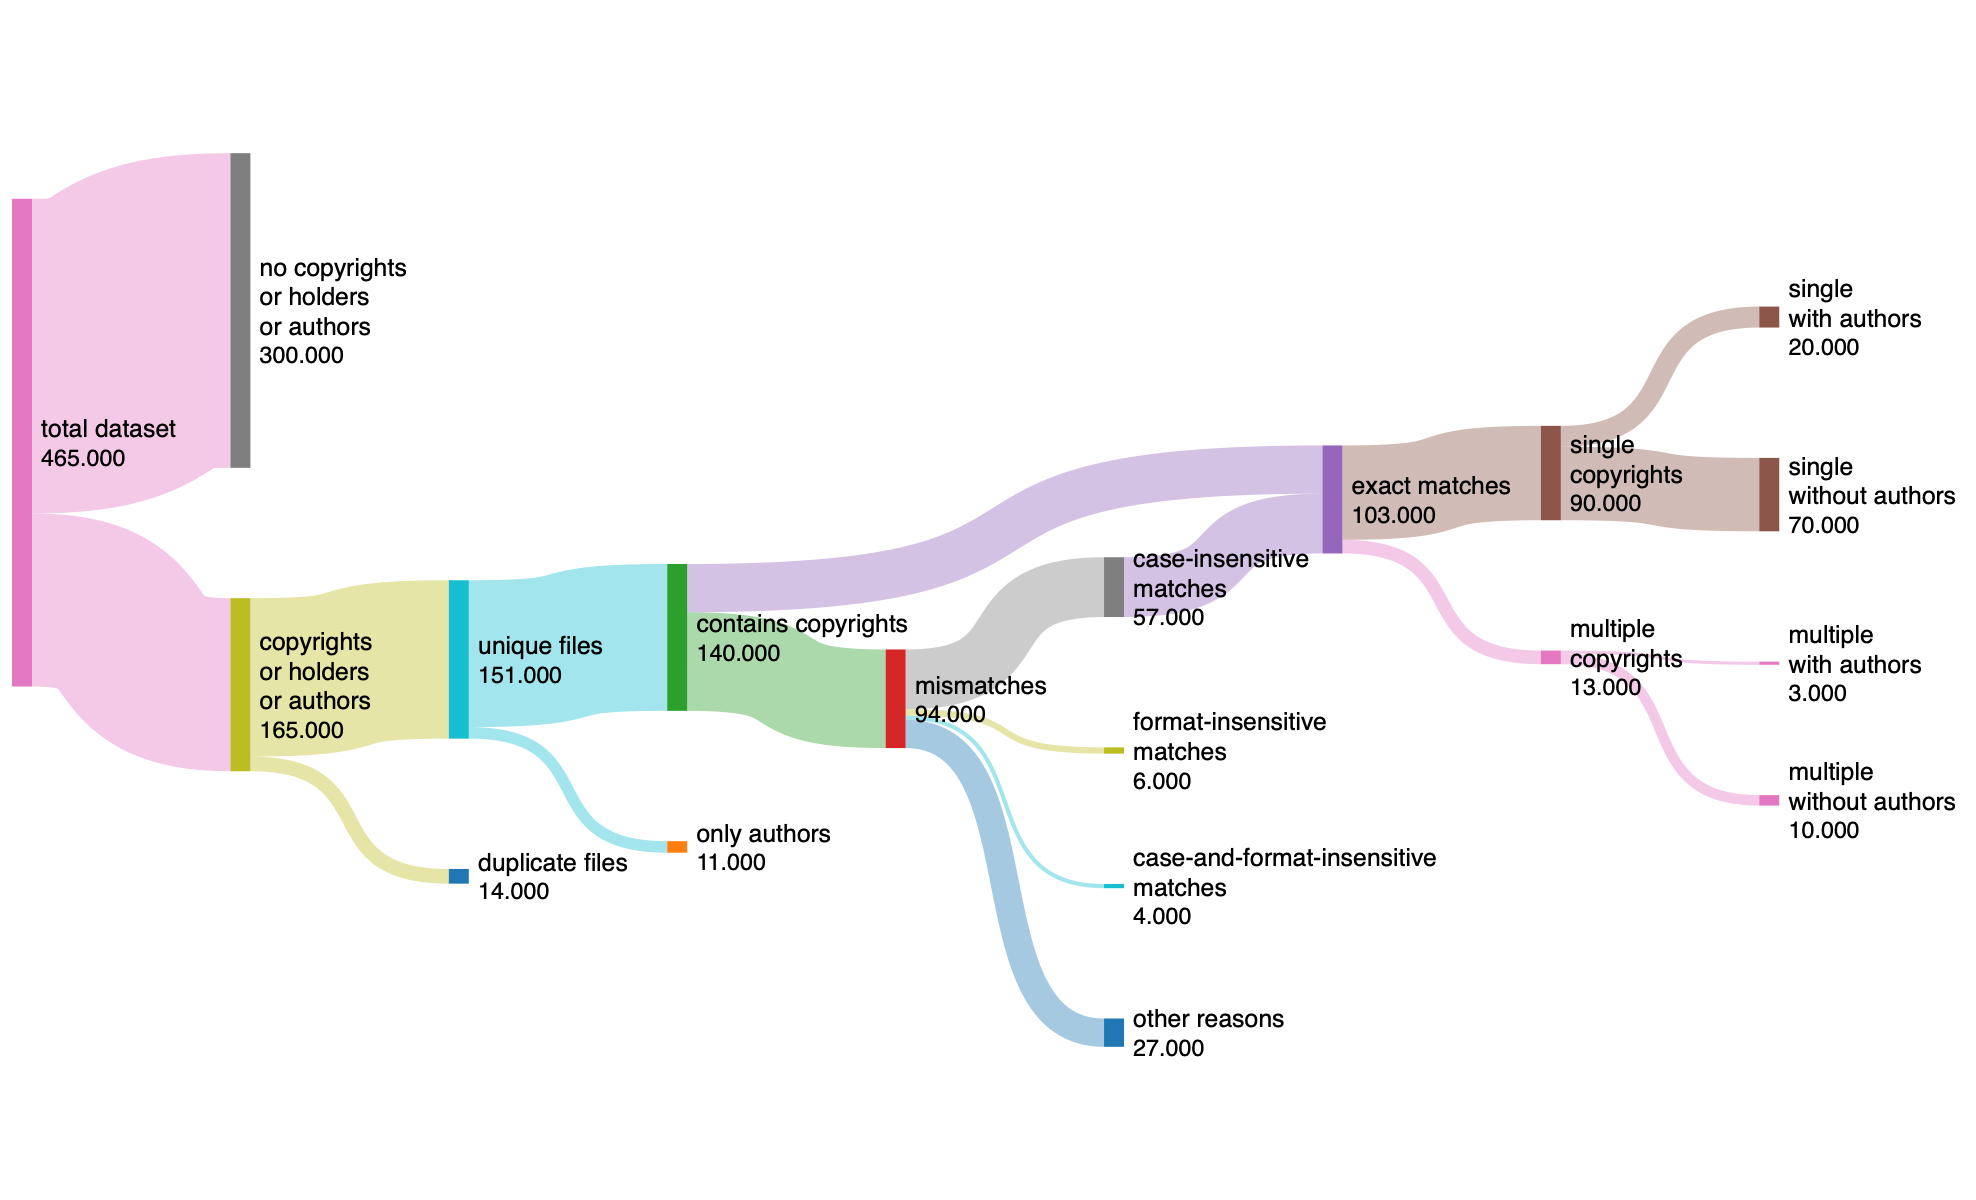
\includegraphics[width=1.3\textwidth]{daten/data-sankey}}
    \caption{
Sankey-Diagramm der Kategorien extrahierter Copyright-Informationen bei der Datenaggregation. Die Darstellung zeigt die schrittweise Reduktion und Klassifikation von \num{465000} Quellcodedateien entlang von Kriterien wie Duplikaterkennung, Copyright-Extraktion, Übereinstimmungsgrad mit den Originaldateien sowie Autorenerkennung. Die Breite der Flüsse entspricht der jeweiligen Anzahl an Dateien pro Kategorie.}
    \label{fig:data-sankey}
\end{figure}
Das Resultat der Datenaggregation sind zehn Hauptkategorien von Dateien, welche unterschiedliche Qualitätsstufen in Hinsicht auf die Policy und auf den Aufwand in ihrer Nachbereitung aufweisen.
Die \autoref{fig:data-sankey} veranschaulicht die schrittweise Verarbeitung und Kategorisierung der Daten.
Besonders bei der Abbildung hervorzuheben ist die Zusammenführung der \textit{exact matches} und der rekonstruierten \textit{case-insensitive matches}, welche den größten Anteil des Datensatzes ausmachen.
Die aggregierten Kategorien dienen in den folgenden Untersuchungen dazu, möglichst heterogene Testdaten zu wählen und dabei möglichst viele Arten von Copyrights zu prüfen.

% ======================================================================================================================

% Hier soll darauf eingegangen werden, welche Probleme und Herausforderungen der Datensatz mit sich gebracht hat, einige
% davon sind die Größe (170GB), die Encodings, Binary-Dateien und die geringe Qualität der Scancode extraktion im "authors" Feld.
\section{Herausforderungen bei der Datenaggregation}\label{sec:herausforderungen-datenaggregation}

Die Verarbeitung der Daten brachte einige Schwierigkeiten mit sich.
Der ursprüngliche Datensatz umfasste ca.\ 170 Gigabyte an Quellcode-Dateien und Ergebnisdaten.
Die automatische Analyse einer solchen Datenmenge erfordert robuste Prozesse und zuverlässige, leistungsfähige Hardware.
Eine weitere Herausforderung bei der Verarbeitung der Daten waren die verschiedenen Encodings der Quellcode-Dateien.
Da es sich beim Datensatz um jede Art von Datentyp und Kodierung handeln kann, muss sichergestellt werden, dass Encodings korrekt erfasst und entsprechend verarbeitet werden.
Im Falle eines nicht klar erkennbaren Encodings wird auf UTF-8 als Default zurückgegriffen.
Neben den Encodings verursachen auch Binär-Dateien zahlreiche Probleme bei der automatischen Auswertung des Datensatzes.
Tritt der Fall auf, dass der Prozess auf eine nicht lesbare Datei stößt, wird diese übersprungen und im weiteren Verlauf nicht berücksichtigt.
Eine verbesserte Version des Datenaggregationsprozesses sollte demnach die korrekte Verarbeitung von Binär-Dateien unterstützen.

% ======================================================================================================================

% Hier soll darauf eingegangen werden, welche Probleme/Qualitätseinbußen der Datensatz aufzuweisen hat, darüber hinaus soll erläutert werden, warum der Datensatz gut ist
% Der Datensatz ist nicht gut weil es keinen besseren gibt -> vielleicht ist ein besserer nur nicht bekannt, stattdessen
% ist der Datensatz mit dem aktuellen Industriestandard (ScanCode) erzeugt worden und wurde nach der von uns erstellten Policy verbessert und validiert
\section{Qualität der Daten}\label{sec:qualitaet-der-daten}

Der aus der Datenaggregation resultierende Datensatz umfasst eine große Anzahl an Dateien die eine Policy-konforme Extraktion von Copyright-Statements aufweisen.
Die \textit{holders} und \textit{authors} dieser Extraktionen sind allerdings nicht geprüft und können aus Sicht der Policy fehlerhaft sein.
Einige der Datenkategorien benötigen außerdem noch manuelle Prüfung bzw.\ Pflege.
Um dennoch korrekte Daten dieser Kategorien zur Verfügung zu haben wurde ein manuell überprüfter Datensatz erstellt.
Die Qualität des Datensatzes ist dadurch gegeben, dass der Ausgangsdatensatz mithilfe des Toolkits erzeugt wurde, welches der aktuelle Industriestandard ist, und anschließend in Form der Datenaggregation Schrittweise verbessert wurde.

\chapter{Benchmark und Modellauswahl}\label{ch:benchmark}

Die systematische Auswahl eines geeigneten \glspl{llm} erforderte die Entwicklung und Anwendung eines spezifisch auf den Anwendungsfall zugeschnittenen Benchmarks.
Die Konzeption und Durchführung war ein iterativer Prozess bei dem stetig Erkenntnisse und identifizierte Probleme dazu genutzt wurden, den Benchmark zu verbessern.
Dieser iterative Prozess hatte zur Folge, dass aufbauend auf Zwischenergebnisse Anpassungen vorgenommen wurden.
Deshalb wird in den folgenden Unterkapiteln nicht nur auf das finale Ergebnis des Benchmarks, sondern auch auf die Zwischenergebnisse und die daraus abgeleiteten Entscheidungen eingegangen.

% ======================================================================================================================

\section{Auswahl der Sprachmodelle}\label{sec:modelle-benchmark}

Die Auswahl an verfügbaren \glspl{llm} wird einerseits durch die Leistungsfähigkeit der verwendeten Hardware und andererseits durch die Kompatibilität der Software eingeschränkt.
Erste Experimente ergaben, dass der verwendete Mac Mini M4 Pro mit 64 Gigabyte Arbeitsspeicher \glspl{llm} mit einer Parametergröße von maximal 108 Milliarden ausführen kann, ohne wärmebedingt die Leistung zu drosseln.
Da die finale Implementierung des Benchmarks softwareseitig mit Ollama4J einen lokal ausgeführten Ollama Server anspricht, konnten nur solche \glspl{llm} ausgewählt werden, die auf Ollama zur Verfügung stehen.
Die Wahl an \glspl{llm}, die für den Benchmark genutzt werden sollen, beschränkt sich somit auf Modelle die durch Ollama unterstützt werden und bis zu 108 Milliarden Parameter groß sind.
Es wurden \glspl{llm} von zahlreichen namhaften Providern geprüft, darunter Microsoft (phi4, phi3), Meta (llama4, llama3), Deepseek (deepseek-coder, deepseek-r1), Alibaba (qwen3, qwen2.5, qwen2.5-coder), Google (gemma3, gemma3n) und Mistral (mistral, mathstral, devstral, mistral-small, mistral-nemo).
Zusätzlich zu etablierten Modellen wurden auch gezielt exotischere und weniger verbreitete Modelle ausgewählt (llava, olmo2, orca-mini, dolphin).
Neben den Providern spielte auch die ausgeschriebene Verwendung der Modelle eine Rolle, somit wurden Modelle für verschiedene Anforderungen wie Vision (llava), Reasoning (qwen3, mixstral) und Programmierung (devstral, qwen2.5-coder) ausgewählt.
Um einen Vergleich in Hinsicht auf Präzision und Performance anhand der Modellgröße zu ermöglichen, wurden gezielt kleine Modelle (tinyllama:1.1b, orca-mini:3b, qwen2.5-coder:0.5b), mittelgroße Modelle (mistral-small:24b, qwen2.5-coder:32b) und große Modelle (llama4:108.6B, mixstral:8x7b) verglichen.
Die finale Durchführung des Benchmarks umfasste 30 \glspl{llm}.

% ======================================================================================================================

\section{Konzeption}\label{sec:konzeption-benchmark}

Ziel des Benchmarks ist es, ein geeignetes \gls{llm} zu bestimmen.
Es wird geprüft, inwiefern das \glspl{llm} Copyright-Informationen extrahieren kann, die Policy-konformen Erwartungshaltungen entsprechen.
Hierzu wird das \gls{llm} mit einem Prompt dazu aufgefordert, die Copyright-Statements, Urheber und Autoren für eine bestimmte Eingangsdatei zu bestimmen und anschließend wird die generierte Ausgabe mit einer vorher formulierten Erwartungshaltungen abgeglichen.
Dieser Schritt wird für jede Datei des Datensatzes durchgeführt.
Der verwendete Datensatz wird im Abschnitt \nameref{sec:datensatz-benchmark} thematisiert.

% ----------------------------------------------------------------------------------------------------------------------

\subsection{Lokale Ausführung der LLMs}\label{subsec:lokale-ausfuehrung}

Um konsistente Ergebnisse über mehrere Durchläufe hinweg zu erzielen, muss sichergestellt werden, dass die Ausgaben der Modelle für denselben Prompt bei mehrmaliger Durchführung nicht variieren.
Hierzu wird die Temperatur der \glspl{llm} auf 0,0 gestellt.
Diese Einstellung ermöglicht es, die Varianz zwischen den Ausgaben, welche bei kreativer Textgenerierung durchaus erwünscht ist, zu eliminieren und sorgt somit für eine deterministische Ausgabe.
Die Funktionalität der Temperatur wurde praktisch geprüft, indem ein Modell in einer bestimmten Größe und Version auf zwei verschiedenen Endgeräten mit demselben Prompt angewiesen wurde und in beiden Fällen eine identische Ausgabe generierte.
Um sicherzustellen, dass im Verlauf des Benchmarks und darüber hinaus keine Updates der Modelle die Ergebnisse verfälschen, müssen feste Versionen der \glspl{llm} verwendet werden.
Da proprietäre \glspl{llm} wie ChatGPT oder Gemini keine Steuerung der Versionen oder Temperatur ermöglichen, ist eine lokale Ausführung der Modelle erforderlich.
Außerdem fallen für die Nutzung der \gls{api} dieser Modelle kosten an, weshalb eine lokale Ausführung auch hier zu bevorzugen ist.
Allerdings erfordert die lokale Ausführung der Modelle, dass diese auf der vorhandenen Hardware lauffähig sind, dies beschränkt die Auswahl der Modelle auf kleinere Parametergrößen und durch \gls{glos:quantisierung} verkleinerte Modelle.

% ======================================================================================================================

\section{Implementierung}\label{sec:benchmark-implementierung}

% Nutzung von TextSieve
% Model Warmup
% Parsing von JSON durch ChatUtil
% Ollama4J verwendet
% Timeout von 5 Minuten mit Single-Thread Executor Service

% ======================================================================================================================

\section{Zusammenstellung des Datensatzes}\label{sec:datensatz-benchmark}

Die Ergebnisse der Datenaggregation wurden dazu genutzt, einen kuratierten Benchmark-Datensatz zu erstellen.
Hierzu wurden repräsentative Fälle aus der Datenaggregation identifiziert und ihre Erwartungshaltung anhand der Policy überprüft und, wenn nötig, angepasst.
Der Datensatz umfasst insgesamt $n=200$ Dateien und ihre überprüften Erwartungshaltungen.
Die \num{200} Dateien sind in acht Kategorien mit jeweils \num{25} Dateien unterteilt:

\begin{itemize}
    \item single copyrights with authors
    \item single copyrights without authors
    \item multiple copyrights with authors
    \item multiple copyrights without authors
    \item case-insensitive matches
    \item format-insensitive matches
    \item only authors
    \item no copyrights or authors or holders
\end{itemize}

Die ersten vier Kategorien stellen die \enquote{normalen} Fälle dar, wobei die \textit{case-insensitive} und \textit{format-insensitive} Fälle speziell die Normalisierungen des ScanCode-Toolkits abdecken.
Die Kategorien \textit{no copyrights or authors or holders} und \textit{only authors} dienen gezielt dazu, das Verhalten des Modells bei Abwesenheit von Copyright-Statements zu untersuchen sowie die alleinige Autorenextraktion.
Um repräsentative Fälle einer Kategorie zusammenzustellen wurden je \num{25} Dateien aus den Hauptkategorien des Datensatzes zufällig ausgewählt und anschließend gesichtet.
Ähnliche Fälle (z.B.\ mehrere Copyright-Statements desselben Urhebers) wurden identifiziert und entsprechend ersetzt.
Somit konnte sichergestellt werden, dass kein Copyright, Urheber oder Autor überrepräsentiert im Datensatz vorkommt.
Die relativ kleine Anzahl von Dateien wurde dadurch kompensiert, dass mithilfe der Kategorien möglichst unterschiedliche Arten von Statements und Autoren im Benchmark enthalten sind.
Darüber hinaus ist jede Kategorie mit derselben Anzahl an Dateien vertreten, wodurch eine Bevorzugung bzw.\ Benachteiligung eines Modells anhand ungleichmäßiger Verteilung von Fällen zusätzlich mitigiert wird.
Die Formulierung der Erwartungshaltungen der ausgewählten Dateien wurde anhand einer reduzierten Policy durchgeführt.
Die reduzierte Policy enthielt lediglich die \nameref{subsec:cir-01}, sowie die \nameref{subsec:cep-01} und \nameref{subsec:cep-02}, wobei die \nameref{subsec:hir-01} und \nameref{subsec:air-01} implizit umgesetzt wurden, da sie zu diesem Zeitpunkt noch nicht formuliert waren.

% ======================================================================================================================

\section{Metriken}\label{sec:metriken-benchmark}

Eine systematische Analyse der Eignung mehrerer \glspl{llm} erfordert mehrere Metriken die zur Evaluation herangezogen werden.
Die in diesem Benchmark verwendeten Metriken werden nachfolgend erläutert dabei werden die generierten Ergebnisse des \gls{llm} wie folgt interpretiert:
\begin{itemize}
    \item \textit{\gls{tp}} -- ein Element aus der Erwartungshaltung wird korrekt extrahiert (entweder exakte oder ausreichend ähnliche Übereinstimmung). Sofern ein \gls{tp} für ein Element aus der Erwartungshaltung gefunden wurde, wird dieses Element für die weitere Bewertung ausgeschlossen da jedes Element nur einmalig zugewiesen werden kann.
    \item \textit{\gls{fp}} -- ein vom Modell extrahiertes Element ist nicht in der Erwartungshaltung enthalten oder es ist verbleibt kein ausreichend ähnliches Element.
    \item \textit{\gls{fn}} -- ein Element aus der Erwartungshaltung wird vom Modell nicht extrahiert (weder exakte noch ausreichend ähnliche Übereinstimmung).
\end{itemize}

\subsection{Exact Matches}
Die zentrale Metrik zur Bewertung der Extraktion von Copyright-Statements ist der Anteil sogenannter \textit{Exact Matches}.
Ein \textit{Exact Match} liegt vor, wenn ein vom \gls{llm} generiertes Statement exakt mit einem Statement der vorher formulierten Erwartungshaltung übereinstimmt.
Durch eine perfekte Extraktion ohne zusätzliche Zeichen oder fehlerhafte Normalisierungen wird die \nameref{subsec:cep-01} erfüllt.
Mehrere Studien nutzen \textit{Exact Matches} als Bewertungsmaß für die Leistung von \gls{ner}- und \gls{ie}-Systemen auf Basis von \glspl{llm} \autocite{dunn_structured_2022}\autocite{hu_improving_2024}.

\subsection{F1-Score}
Eine gängige Metrik zur Bewertung von Klassifikationsmodellen ist der F1-Score\autocite{noauthor_f-score_2025}.
Der F1-Score stellt das harmonische Mittel aus Präzision (\textit{P}) und Recall (\textit{R}) dar.
Die Formeln für \textit{P}, \textit{R}, und \textit{F1} lauten wie folgt:

\[
 P = \frac{\mathrm{TP}}{\mathrm{TP} + \mathrm{FP}}
\]

\[
 R = \frac{\mathrm{TP}}{\mathrm{TP} + \mathrm{FN}}
\]

\[
 F1 = 2 \times \frac{P \times R}{P + R}
\]

Außerdem wird ein kombinierter F1-Score aller Elemente einer Eingabe (\enquote{overall F1}) berechnet:

\[
 \mathrm{overall F1} = \frac{\mathrm{copyrightF1} + \mathrm{holderF1} + \mathrm{authorF1}}{3}
\]

In diesem Benchmark wird für jeden Entitätstyp der jeweilige F1-Score berechnet und zusätzlich ein durchschnittlicher F1-Score über alle Typen hinweg erfasst.
Zunächst wird jedes extrahierte Copyright-Statement auf einen \textit{Exact Match} mit der Erwartungshaltung geprüft, liegt dieser vor, wird das Statement als \gls{tp} gezählt.
Sofern kein \textit{Exact Match} vorliegt, wird die Jaro-Winkler-Ähnlichkeit\autocite{noauthor_jarowinkler_nodate} verwendet um das ähnlichste Element aus der Erwartungshaltung welches einen Similarity-Threshold vom \num{0,95} überschreitet, zu finden.
Wenn eine solche Übereinstimmung gefunden wird, zählt diese als \gls{tp}.
Bei Holders und Authors wird ausschließlich durch die Jaro-Winkler-Ähnlichkeit auf ähnliche Elemente in der Erwartungshaltung geprüft und entsprechende Fälle werden als \gls{tp} gezählt.

\subsection{Tokens/sec}
Zur zeitlichen Messung der Modellleistungen werden die \textit{Tokens/sec} berechnet.
Da Ollama4J keine Abfrage der tatsächlichen Token pro Sekunde eines Modells unterstützt muss eine Alternative herangezogen werden.
Um die Leistung der unterschiedlichen Modelle zu bestimmen, wird berechnet wie groß der Eingabe-Prompt ist und wie viel Zeit das Modell zur Bearbeitung benötigt.
Die größe eines Prompts wird in Tokens gemessen, da die Modelle aber intern unterschiedliche Prozesse zur Tokenisierung eines Prompts verwenden, wird eine Annäherung verwendet.
Eine grobe Umrechnung von Eingabetext zu Tokens ist $1\;\text{Token}\approx 4\;\text{Buchstaben}$\autocite{noauthor_what_nodate}.
Die Dauer der Bearbeitung entspricht der Zeit zwischen dem Absenden des Eingabe-Prompts und der Beantwortung durch das Modell.
Die somit ermittelte Metrik stellt eine Vergleichbarkeit der Modell-Geschwindigkeit für alle \glspl{llm} dar, unabhängig von ihrer internen Tokenisierung.

% ======================================================================================================================

\section{Durchführung}\label{sec:durchfuhrung-benchmark}

% ----------------------------------------------------------------------------------------------------------------------

\subsection{Eingabeprompt}

% ======================================================================================================================

\section{Ergebnisse}\label{sec:ergebnisse-benchmark}

% ======================================================================================================================

\section{Wahl des Modells}\label{sec:auswahl-modell-benchmark}


\chapter{Prompt-Engineering}\label{ch:prompt-engineering}

Im vorherigen Kapitel wurden mehrere \glspl{llm} anhand des entwickelten Benchmarks und einer reduzierten Version der Policy miteinander verglichen.
Auf Grundlage dieser Evaluation wurde \texttt{mistral-small:24b} als Modell zur weiteren Untersuchung und Vertiefung der Forschung ausgewählt.
Die Untersuchung wird in diesem Kapitel auf die vollständige Policy ausgeweitet.
Während im Benchmark ausschließlich die reduzierte Policy mit den Anforderungen \nameref{subsec:cir-01}, \nameref{subsec:cep-01} und \nameref{subsec:cep-02} zur Extraktion verwendet wurde und die Erwartungshaltungen dementsprechend auf diese Teilmenge beschränkt waren, werden im weiteren Verlauf dieser Untersuchung die Erwartungshaltungen so erweitert, dass alle Aspekte berücksichtigt werden, mit Ausnahme der mit \enquote{out of scope} (\nameref{subsec:cir-02}, \nameref{subsec:cep-04}, \nameref{subsec:cep-06}) gekennzeichneten Regeln.
Darauf aufbauend wird durch systematisches Prompt-Engineering eine Optimierung der Extraktionsleistung angestrebt.
Ziel ist es, die Extraktion auf Grundlage der gesamten Policy in einer möglichst hohen Qualität zu ermöglichen.
Die Struktur des Prompts, die Formulierung der Entitätsdefinitionen sowie die Gestaltung der Few-Shot-Beispiele werden dabei schrittweise verfeinert, um die Genauigkeit der Extraktion sukzessive zu erhöhen.

% ======================================================================================================================

\section{Methodisches Vorgehen}\label{sec:methodisches-vorgehen}

Einen methodischen Bezugspunkt bildet die Arbeit von \citeauthor{cheng_novel_2024} \autocite{cheng_novel_2024}, in der ein neuartiges Prompting-Verfahren für Few-Shot \gls{ner} vorgestellt wird.
Das Vorgehen der Autoren basiert auf einer klar strukturierten Gestaltung des Prompts, die mehrere aufeinander abgestimmte Bestandteile umfasst.
Zunächst wird eine Aufgabenbeschreibung formuliert, die das \gls{llm} explizit in die Rolle eines Entity-Recognition-Systems versetzt und die Aufgabe eindeutig umreißt.
Darauf folgt eine präzise Definition der Entitätskategorien, die jeweils mit kurzen Erklärungen versehen werden, um semantische Abgrenzungen zwischen den Klassen deutlich zu machen.
Im nächsten Schritt werden Few-Shot-Beispiele integriert, die als Input-Output-Paare gestaltet sind und sowohl die Extraktion selbst als auch das gewünschte Ausgabeformat illustrieren.
Dieses Ausgabeformat wird zusätzlich separat spezifiziert, sodass das Modell konsistente und strukturierte Ergebnisse erzeugt.
Ergänzend sehen \citeauthor{cheng_novel_2024} \autocite{cheng_novel_2024} die Möglichkeit vor, zusätzliche Instruktionen in den Prompt einzufügen, die wiederkehrende Fehlerquellen adressieren und dadurch die Zuverlässigkeit der Ergebnisse erhöhen \autocite{cheng_novel_2024}.

Zur Optimierung dieses Setups führen die Autoren eine Feedback-Schleife ein.
Das \gls{llm} wird mit dem initialen Prompt auf Trainingsdaten angewandt, die Extraktionen durch das \gls{llm} werden mit den Erwartungshaltungen verglichen und anhand des F1-Scores bewertet.
Anschließend werden die am besten verarbeiteten Beispiele identifiziert und als Demonstrationen in den Prompt übernommen.
Auf diese Weise wird der Prompt iterativ verbessert und stärker auf die spezifischen Anforderungen des Tasks zugeschnitten \autocite{cheng_novel_2024}.

Das Vorgehen in dieser Arbeit orientiert sich in seiner Grundstruktur an der Methodik von \citeauthor{cheng_novel_2024} \autocite{cheng_novel_2024}.
Der Prompt ist ebenfalls in mehrere Komponenten gegliedert, bestehend aus einer Aufgabenbeschreibung, präzisen Entitätsdefinitionen, Beispielen, zusätzlichen Instruktionen sowie einem festgelegten Ausgabeformat.
Die Optimierung wurde iterativ durchgeführt, indem die Definitionen schrittweise angepasst und Beispiele ergänzt wurden, die in vorherigen Versionen zu Fehlern bei der Extraktion geführt hatten.

Ein wesentlicher Unterschied zum Vorgehen von \citeauthor{cheng_novel_2024} \autocite{cheng_novel_2024} besteht darin, dass die Auswahl der Beispiele nicht automatisiert über eine Selektion der besten Beispiele anhand von F1-Scores erfolgte, sondern manuell vorgenommen wurde.
Grundlage dieser Anpassungen war eine gezielte Analyse typischer Fehlerkonstellationen, die sich im Benchmark gezeigt haben.
Diese Vorgehensweise wurde gewählt, da zunächst die Optimierung der Ergebnisse innerhalb des entwickelten Benchmarks im Vordergrund steht, um auf dieser Grundlage die Generalisierbarkeit des Modells auf bislang nicht gesehene Daten zu unterstützen.
Ein vergleichbares Vorgehen kam bereits bei der Erstellung des Benchmark-Prompts zur Anwendung, welcher ebenfalls nach einer Reihe explorativer Experimente manuell angepasst und verfeinert wurde, um die Anforderungen der reduzierten Policy abzubilden.

% ======================================================================================================================

\section{Ergebnisse}

Abbildung~\ref{fig:prompt-engineering-results} zeigt die Resultate des Prompt-Engineerings.
Für die verschiedenen Versionen des Prompts werden zwei Metriken dargestellt.
Einerseits der Prozentsatz der \textit{Exact Matches} und andererseits der \textit{F1-Score}, dessen Werte mit dem Faktor \num{100} multipliziert wurden, um eine direkte Vergleichbarkeit mit den \textit{Exact Matches} zu ermöglichen.
Von Version \texttt{P0} bis \texttt{P7} steigt der Anteil an \textit{Exact Matches} kontinuierlich an, während der \textit{F1-Score} ab Version \texttt{P5} ein Plateau erreicht.
Die Version \texttt{P7.2} erzielt mit \num{96.27} \% den höchsten Wert an \textit{Exact Matches} bei einem \textit{F1-Score} von \num{0.9336}.

\begin{figure}[ht]
    \centering
    \makebox[\textwidth]{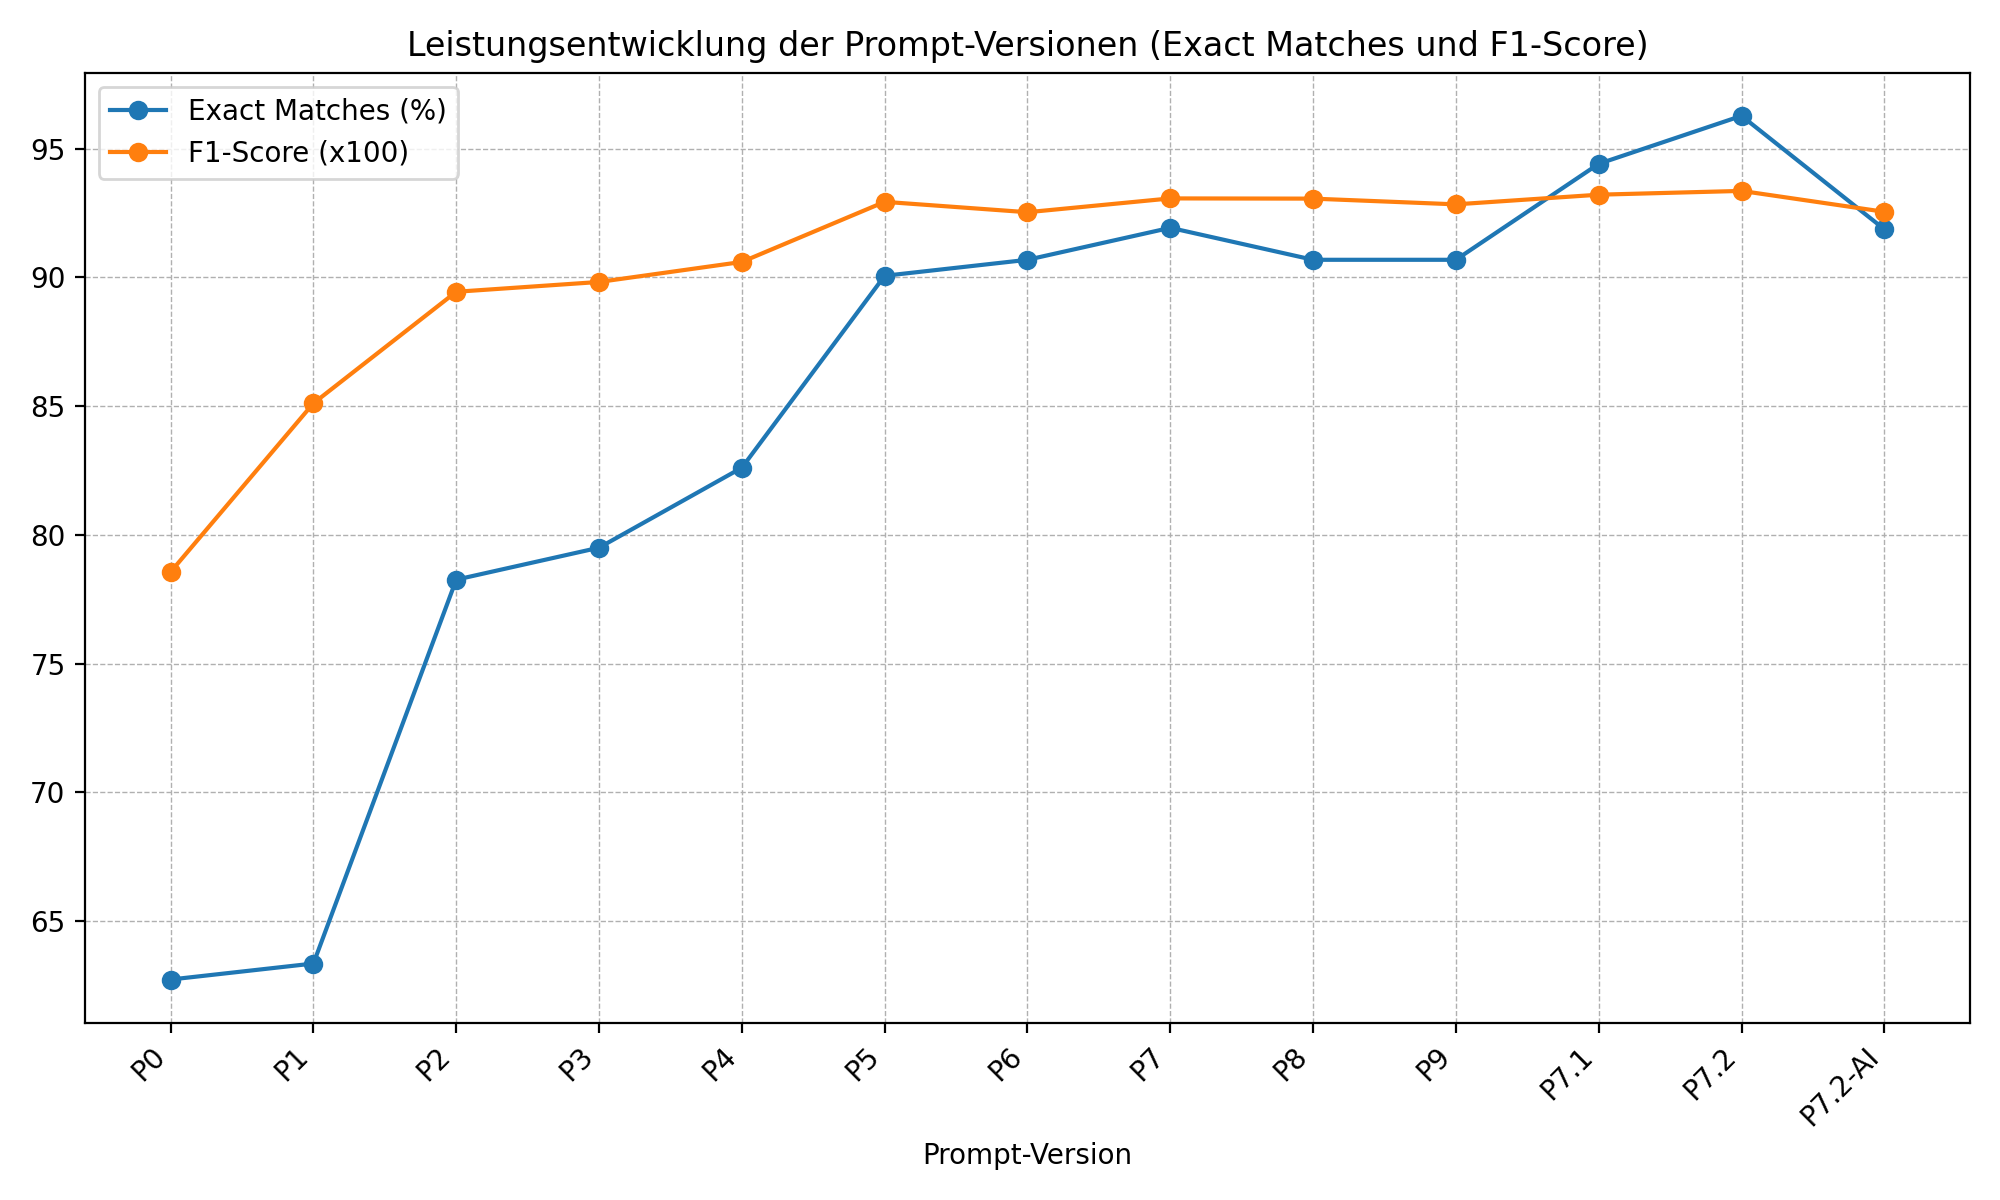
\includegraphics[width=1.3\textwidth]{prompt-engineering/prompt_versions_performance.png}}
    \caption{Entwicklung der Extraktionsleistung über die verschiedenen Prompt-Versionen. Dargestellt sind die Exact Matches und die F1-Scores (multipliziert mit 100). Die Werte steigen bis Version P7 kontinuierlich an, wobei die Version P7.2 die besten Ergebnisse erzielt.}
    \label{fig:prompt-engineering-results}
\end{figure}

Der Prompt \texttt{P0} stellt den Ausgangspunkt dar, mit dem der Benchmark durchgeführt wurde.
Erwartungsgemäß erreicht diese Version mit \num{62.73} \% einen niedrigen Wert bei den \textit{Exact Matches}, da sie ausschließlich auf der reduzierten Policy basierte.
In den Versionen \texttt{P1} bis \texttt{P9} wurden die Entitätsdefinitionen sukzessive erweitert, sodass die zusätzlichen Aspekte der vollständigen Policy berücksichtigt wurden.
In \texttt{P1} wurden zunächst Erklärungen aufgenommen, die den Anforderungen \nameref{subsec:cep-03}, \nameref{subsec:gep-01} und \nameref{subsec:air-01} entsprechen.
Mit \texttt{P2} kamen Definitionen für die \nameref{subsec:aep-01} und die \nameref{subsec:hep-01} hinzu.
Zusätzlich wurden Beispiele konstruiert, die \textit{Authors} und \textit{Holders} mit E-Mail-Adressen beinhalten und damit \nameref{subsec:gep-01} abbilden, sowie Beispiele, die Blöcke von Copyright-Statements enthalten und damit \nameref{subsec:cep-03} berücksichtigen.
Dabei wurde sichergestellt, dass die Beispiele keine Inhalte umfassen, die Teil des Benchmarks sind, um Überschneidungen zwischen Trainings- und Testdaten zu vermeiden.

In \texttt{P3} wurden weitere Beispiele ergänzt.
Da das \gls{llm} Schwierigkeiten bei der korrekten Erkennung von Blockstrukturen mit mehreren Copyrights zeigte, wurde in \texttt{P4} die Definition dieser Struktur präzisiert.
Mit \texttt{P5} wurde ein Beispiel für einen umfangreichen Block mit sechs Copyright-Statements hinzugefügt sowie ein Beispiel, das irrelevante Lizenzhinweise enthält, die bei der Extraktion nicht übernommen werden sollten.

Die Versionen \texttt{P7} bis \texttt{P9} wurden vor allem durch zusätzliche Beispiele erweitert.
Während der Anteil an \textit{Exact Matches} in \texttt{P7} den höchsten Wert dieser Serie erreichte, sank er in den nachfolgenden Versionen wieder leicht ab.
Daher wurde die Version \texttt{P7} erneut aufgegriffen und als Grundlage für weitere Optimierungen genutzt.
Diese Erweiterungen erfolgten durch zusätzliche Instruktionen nach den Few-Shot-Beispielen, wie sie auch von \citeauthor{cheng_novel_2024}\ empfohlen werden \autocite{cheng_novel_2024}.

In den Versionen \texttt{P7.1} und \texttt{P7.2} wurden ergänzende Erklärungen integriert, die klarstellen, dass Lizenzinformationen nicht Teil der Copyrights sind und dass Kommentarsyntax vor und nach den Statements zu vermeiden ist.
Außerdem wurde ein weiteres Beispiel aufgenommen, das die korrekte Extraktion von Statements in Ascii-Art verdeutlicht.
Die Version \texttt{P7.2} enthält insgesamt sieben Few-Shot-Beispiele und wird für die nachfolgenden Untersuchungen verwendet.
Der vollständige Prompt ist im Anhang~\ref{sec:anahng-prompt-p7.2} aufgeführt.

% TODO: Prompt und Ergebnis des LLMs korrekt in Anhang aufzeigen
Im Anschluss wurde ein Experiment mit GPT-5 \footnote{\url{https://openai.com/index/introducing-gpt-5/}} durchgeführt, bei dem das Modell aufgefordert wurde, den Prompt \texttt{P7.2} zu optimieren.
Der resultierende Prompt ist als \texttt{P7.2-AI} in den Ergebnissen gekennzeichnet und im Anhang~\ref{sec:anahng-prompt-p7.2-ai} hinterlegt.
Die wesentliche Änderung bestand darin, dass die Beschreibungen der Entitäten in eine stichpunktartige Struktur umgewandelt und sprachlich leicht angepasst wurden.
Die Ergebnisse zeigen jedoch, dass diese Anpassung einen geringeren Anteil an \textit{Exact Matches} von \num{91.86} \% zur Folge hatte.

% ======================================================================================================================

\section{Validierung mit ungesehenen Daten}

Nachdem im Rahmen des Benchmarks eine Optimierung des Eingabeprompts durchgeführt wurde, erfolgte im nächsten Schritt eine Validierung mit bisher ungesehenen Daten.
Zu diesem Zweck wurde ein Datensatz zusammengestellt, der aus \num{200} Dateien der Kategorie \enquote{single copyrights without authors} sowie \num{200} Dateien der Kategorie \enquote{multiple copyrights with authors} besteht.
Für alle Dateien wurden die Erwartungshaltungen gemäß der vollständigen Policy definiert.
Bei der Kuratierung wurde darauf geachtet, dass jedes Copyright-Statement nur einmal im Datensatz vorkommt, um Wiederholungen zu vermeiden.

Die Extraktion der \enquote{single copyrights without authors} erreichte einen Wert von \num{99} \% \textit{Exact Matches}, was auf eine sehr gute Generalisierungsfähigkeit der optimierten Lösung in diesem einfachen Szenario hinweist.
Im Fall der \enquote{multiple copyrights with authors} lag der Anteil an \textit{Exact Matches} hingegen lediglich bei \num{73.88} \%.
Dieses Ergebnis verdeutlicht, dass die Optimierung zwar für einfache Extraktionsaufgaben eine robuste Leistung erzielt, bei komplexeren Strukturen mit mehreren Statements und Autoren jedoch noch deutliche Einschränkungen bestehen.

% ======================================================================================================================

\section{Analyse der ScanCode False-Negatives}

Da der Vergleich zwischen dem ScanCode-Toolkit und der \gls{llm}-basierten Lösung einen zentralen Bestandteil dieser Arbeit darstellt, wurde ein isoliertes Experiment durchgeführt.
Aus der Kategorie \enquote{no copyrights or authors or holders} des Datensatzes wurden \num{3000} Dateien zufällig ausgewählt und auf das Vorkommen von Copyright-Statements untersucht.
Diese Kategorie umfasst Dateien, in denen das ScanCode-Toolkit keine Copyright-Informationen identifizieren konnte.
Ziel der Analyse war daher zu prüfen, ob die optimierte \gls{llm}-Lösung in diesen Fällen dennoch Copyright-Statements extrahieren kann, die als False-Negatives des ScanCode-Toolkits zu interpretieren sind.

Die Untersuchung ergab, dass die optimierte \gls{llm}-Lösung insgesamt \num{20} Copyright-Statements extrahieren konnte.
Der Großteil dieser Funde stammt aus Binärdateien, was darauf hindeutet, dass das \gls{llm} im Gegensatz zum regelbasierten Ansatz des ScanCode-Toolkits in der Lage ist, auch in diesem Dateityp relevante Informationen zu erkennen.

Darüber hinaus wurde ein weiterer Fall entdeckt, bei dem ein Copyright-Statement in einer HTML-Datei durch das ScanCode-Toolkit nicht erkannt wurde:

\begin{lstlisting}[keepspaces=true]
[...]
REVISION
</b><br>
<P>
Last updated: 12 October 2023
<br>
Copyright &copy; 1997-2023 University of Cambridge.
<br>
<p>
Return to the <a href="index.html">PCRE2 index page</a>.
</p>
\end{lstlisting}

Die \gls{llm}-Lösung extrahierte hierbei folgende Informationen:

\begin{lstlisting}[keepspaces=true]
{
    "copyrights": ["Copyright &copy; 1997-2023 University of Cambridge."],
    "holders": ["University of Cambridge"],
    "authors": ["Philip Hazel"]
}
\end{lstlisting}

Dies ist ein Anzeichen dafür, dass es eventuell weitere Strukturen von Copyright-Statements gibt, die das ScanCode Toolkit derzeit nicht erkennt, welche aber durch das semantische Verständnis des \gls{llm} korrekt identifiziert werden können.
Eine tiefgreifendere Analyse der False-Positives könnte weitere solcher Fälle aufzeigen und zur Erweiterung des Testdatensatzes besonders relevant sein.
Weiterhin könnte dieser Ansatz der gegenläufigen Prüfung auch bei anderen Datenkategorien zur Identifikation besonderer Fälle und zur weiteren Schärfung der Policy genutzt werden.
\chapter{Fine-Tuning}\label{ch:fine-tuning}

Aufbauend auf den Ergebnissen des Prompt-Engineerings wird in diesem Kapitel das Training eines \gls{llm} für die Extraktion von Copyright-Statements untersucht.
Da das vollständige Fine-Tuning von \glspl{llm} mit erheblichem Ressourcenaufwand verbunden ist, wird stattdessen ein Ansatz mit \gls{lora} gewählt.
Um den Speicherbedarf weiter zu reduzieren und die Effizienz zu erhöhen, wird das Training mit quantisierten \glspl{llm} durchgeführt (QLoRA).

Ziel dieser Untersuchung ist es herauszufinden, ob ein Modell durch Fine-Tuning in der Lage ist, die Anforderungen einer Policy implizit aus umfangreichen Beispieldaten zu lernen, wodurch auf explizite Instruktionen, wie sie beim Prompt-Engineering erforderlich waren, verzichtet werden kann.

\section{Durchführung}

Für die Umsetzung des Fine-Tunings wird das Framework MLX\footnote{\url{https://github.com/ml-explore/mlx}} von Apple eingesetzt, das speziell für Apple-Silicon-Prozessoren optimiert ist.
Die Experimente wurden auf derselben Hardware durchgeführt wie die vorangegangenen Untersuchungen (Mac Mini M4 Pro).

Die Vorgehensweise orientierte sich maßgeblich an den Referenzimplementierungen aus dem MLX-Examples-Repository\footnote{\url{https://github.com/ml-explore/mlx-examples}}.
Voraussetzung für das Training ist ein Datensatz im JSONL-Format, der in die drei Kategorien \textit{train}, \textit{test} und \textit{valid} gegliedert wird.

\begin{itemize}
    \item \textit{train} enthält die Daten, mit denen das Modell tatsächlich trainiert wird. Nach Empfehlung von MLX sollten etwa \num{80}\% der Gesamtdaten in diesem Teil enthalten sein.
    \item \textit{test} dient der Evaluierung der Trainingsleistung auf bislang ungesehenen Daten und sollte rund \num{10}\% des Datensatzes umfassen.
    \item \textit{valid} wird für die fortlaufende Validierung während des Trainings genutzt. In regelmäßigen Abständen wird so überprüft, ob das Modell die gewünschten Lernfortschritte macht.
\end{itemize}
Jede Zeile des Datensatzes enthält einen Eingabeprompt sowie die dazugehörige erwartete Ausgabe.
Das Training erfolgt, indem das Modell lernt, aus der Eingabe die gewünschte Ausgabe korrekt zu generieren.
Im Gegensatz zur Prompt-Engineering-Lösung wird hierbei keine ausführliche Aufgabenbeschreibung vorgegeben, sondern lediglich eine allgemeine Instruktion.
Diese Instruktion kann bei der Inferenz genutzt werden, um das erlernte Verhalten zuverlässig abzurufen.

MLX stellt verschiedene Parameter zur Steuerung des Trainings bereit.
Von besonderer Bedeutung waren:

\begin{itemize}
    \item \textit{LoRA-Layers}: legt die Anzahl der trainierbaren LoRA-Schichten fest und bestimmt damit die Menge der anzupassenden Gewichte.
    \item \textit{iterations}: gibt an, wie viele Trainingszyklen durchgeführt werden. Pro Iteration wird jeweils ein Batch an Trainingsdaten verarbeitet.
    \item \textit{learning-rate}: bestimmt die Geschwindigkeit, mit der die Modellgewichte angepasst werden.
\end{itemize}

Alle weiteren Parameter wurden unverändert auf den Standardwerten belassen, da eine umfassende Analyse und Optimierung dieser Einstellungen den Rahmen der Arbeit überschritten hätte.

\subsection{Durchführung mit kuratierten Daten}

Für den ersten Fine-Tuning-Durchlauf wurde ein Datensatz verwendet, der ausschließlich aus manuell kuratierten Beispielen der Kategorie \textit{manually checked} bestand.
Der Datensatz umfasst \num{500} qualitativ hochwertige Einträge, die ein breites Spektrum der in der Policy definierten Regeln abdeckten.

Als Basis für das Fine-Tuning wurde das Modell \texttt{mistral-7B-Instruct-v0.3}\footnote{\url{https://huggingface.co/mistralai/Mistral-7B-Instruct-v0.3}} ausgewählt.
Dieses Modell weist eine enge Verwandtschaft zu \texttt{mistral-small:24b} auf, das im Benchmark besonders gute Ergebnisse erzielt hat.
Darüber hinaus handelt es sich um eine Instruct-Variante.
Im Gegensatz zu reinen Basismodellen, die primär auf die Fortsetzung von Text trainiert sind, werden Instruct-Modelle zusätzlich darauf optimiert, Anweisungen präzise zu befolgen und strukturierte Ausgaben zu erzeugen.
Diese Fähigkeit macht sie besonders für Aufgaben wie \gls{ner} geeignet und stellt daher eine geeignete Ausgangsbasis für die vorliegende Untersuchung dar.

Das initiale Training erfolgte mit den Standardparametern von MLX.
Es wurde eine Lernrate von $2 \times 10^{-5}$ bei insgesamt \num{800} Iterationen verwendet.
Obwohl die von MLX bereitgestellten Trainings- und Evaluationsmetriken auf einen erfolgreichen Verlauf hindeuteten, zeigten die praktischen Ausgaben des Modells deutliche Defizite.
Die generierten Ergebnisse bestanden überwiegend aus zusammenhangslosen und unstrukturierten Textfragmenten, die häufig Code-Anteile enthielten und nicht den erwarteten Extraktionen entsprachen.
Auch die anschließende Manipulation der Lernrate, Lora-Schichten und Iterationen bewirkte keine Verbesserung.

\subsection{Durchführung mit generierten Daten}

Die Beobachtungen der ersten Durchführung deuten darauf hin, dass die Größe des verwendeten Datensatzes nicht ausreicht, um ein erfolgreiches Fine-Tuning durchzuführen.
Für die zweite Durchführung wurde daher ein erweiterter Datensatz erstellt.
Zunächst wurden 2000 Dateien der Kategorie \textit{single copyrights without authors} sowie 2000 Dateien der Kategorie \textit{single copyrights with authors} zufällig ausgewählt.
Anschließend wurde die im Kapitel~\ref{ch:prompt-engineering} entwickelte Lösung eingesetzt, um für diese insgesamt 4000 Dateien die Copyright-Informationen zu extrahieren.

Die Eignung dieses Ansatzes basiert auf den zuvor erzielten Ergebnissen, die gezeigt haben, dass die Prompt-Engineering-Lösung bei ungesehenen Daten in der Kategorie \textit{single copyrights} eine Extraktionsgenauigkeit von \num{99}\% an \textit{Exact Matches} erreichen konnte.
Es ist daher davon auszugehen, dass die generierten Trainingsdaten eine hinreichend hohe Qualität aufwiesen, um für ein Fine-Tuning geeignet zu sein.

Der so erstellte Datensatz wurde für das Fine-Tuning des Modells \texttt{mistral-7B-Instruct-v0.3} verwendet.
Das Training erfolgte mit 16 LoRA-Schichten, einer Lernrate von $2 \times 10^{-5}$ und \num{1600} Iterationen, während alle übrigen Parameter unverändert auf den Standardwerten belassen wurden.
Das Modell reagierte nach Abschluss des Trainings korrekt auf die in den Trainingsdaten vorgegebene Instruktion und erzeugte sämtliche Ausgaben konsistent im JSON-Format, ohne Abweichung in der Repräsentation des Formats zu erzeugen.
Die genauen Ergebnisse werden im Abschnitt~\ref{sec:lora-ergebnisse} aufgezeigt.
Der aus dem Training resultierende LoRA-Adapter wurde auf der Plattform Hugging Face\footnote{\url{https://huggingface.co}} veröffentlicht und steht dort zum Download zur Verfügung\footnote{\url{https://huggingface.co/metaeffekt/copyright-scanner-mistral-7b-instruct-v0.3}}.

Da das Fine-Tuning mit einem Modell der Größe von sieben Milliarden Parametern bereits vielversprechende Ergebnisse lieferte, wurde im Anschluss untersucht, ob sich ähnliche Resultate auch mit einem deutlich kleineren Modell erzielen lassen.
Hierfür wurde das Instruct-Modell \texttt{Qwen2.5-1.5B-Instruct}\footnote{\url{https://huggingface.co/Qwen/Qwen2.5-1.5B-Instruct}} ausgewählt.
Das Training erfolgte unter identischen Bedingungen wie zuvor, mit dem Unterschied, dass 28 LoRA-Schichten trainiert wurden, was der maximal möglichen Anzahl bei \texttt{Qwen2.5-1.5B-Instruct} entspricht.
Die Erhöhung der LoRA-Schichten wurde vorgenommen, da das verhältnismäßig kleine \gls{llm} weniger Arbeitsspeicher beim Training beansprucht, was die Möglichkeit eröffnete, die volle Anzahl der verfügbaren Schichten zu verwenden.
Auch dieses Modell war nach Abschluss des Trainings imstande, das korrekte Ausgabeformat zuverlässig zu erzeugen.
Der entsprechende Adapter für dieses Modell wurde ebenfalls auf Hugging Face veröffentlicht\footnote{\url{https://huggingface.co/metaeffekt/copyright-scanner-qwen2.5-1.5b-instruct}}.

Die Ergebnisse der trainierten Modelle werden im folgenden Abschnitt mit den Resultaten der Prompt-Engineering-Lösung verglichen.

\section{Ergebnisse}\label{sec:lora-ergebnisse}

Für die abschließende Bewertung und den Vergleich der Modelle wurde der kuratierte Datensatz herangezogen, der aus \num{200} Dateien der Kategorie \textit{exact matches without authors} besteht.
Dieser Datensatz wurde bereits im Kapitel~\ref{ch:benchmark} verwendet, um die Generalisierbarkeit der Prompt-Engineering-Lösung auf ungesehenen Daten zu analysieren.
Dadurch wurde eine direkte Vergleichbarkeit der Ergebnisse sichergestellt.

Zur Bewertung der Leistung werden die beiden fine-tuned \glspl{llm} mit der Prompt-Engineering-Lösung aus dem vorherigen Kapitel verglichen.
Die zentralen Metriken sind dabei die Qualität der Extraktion, gemessen am prozentualen Anteil der\textit{Exact Matches}, und die Verarbeitungsgeschwindigkeit in \textit{Tokens/sec}.
Tabelle~\ref{tab:modellvergleich} fasst die Ergebnisse zusammen.

\begin{table}[H]
    \centering
    \begin{tabular}{l c c}
        \hline
        \textbf{Modell} & \textbf{Exact Matches (\%)} & \textbf{Tokens/sec} \\
        \hline
        \texttt{mistral-small:24b} & 99,0 & 6,02 \\
        \texttt{mistral:7b-instruct-v0.3-fine-tuned} & 99,0 & 20,93 \\
        \texttt{qwen2.5-1.5b-instruct-fine-tuned} & 91,5 & 71,53 \\
        \hline
    \end{tabular}
    \caption{Vergleich der fine-tuned Modelle mit der Prompt-Engineering-Lösung hinsichtlich Genauigkeit und Geschwindigkeit.}
    \label{tab:modellvergleich}
\end{table}

Wie die Ergebnisse zeigen, erbringt das Modell \texttt{mistral:7b-instruct-v0.3-fine-tuned} eine herausragende Leistung.
Mit einem Anteil von \num{99}\% an \textit{Exact Matches} erreicht es exakt dieselbe Genauigkeit wie das deutlich größere \texttt{mistral-small:24b}.
Gleichzeitig ist die Verarbeitungsgeschwindigkeit mit rund \num{21} \textit{Tokens/sec} mehr als dreimal so hoch wie bei der Prompt-Engineering-Lösung mit ca. \num{6} \textit{Tokens/sec}.
Dieses Ergebnis belegt, dass das Modell die impliziten Regeln der Policy erfolgreich aus den Trainingsdaten erlernen konnte und dabei eine signifikante Effizienzsteigerung erzielt.

Das deutlich kleinere Modell \texttt{qwen2.5-1.5b-instruct-fine-tuned} stellt einen Kompromiss zwischen Genauigkeit und Geschwindigkeit dar.
Die Genauigkeit der Extraktionen sinkt auf \num{91,5}\%, was eine merkliche Reduzierung im Vergleich zu den beiden Mistral-Modellen darstellt.
Im Gegenzug erreicht es mit über \num{71} \textit{Tokens/sec} eine deutlich höhere Verarbeitungsgeschwindigkeit.
Es ist damit mehr als elfmal so schnell wie die ursprüngliche Prompt-Engineering-Lösung.

Ein wesentlicher Vorteil der fine-tuned Modelle liegt in der Vereinfachung der Inferenz.
Statt eines komplexen Prompts von rund 1660 Tokens, wie er für die Prompt-Engineering-Lösung erforderlich war, genügt nun die einfache Anweisung: \enquote{Extract the copyrights, holders and authors in JSON format from the following file} (ca. 20 Tokens).
Zudem erzeugen die Modelle konsistent gültige JSON-Ausgaben, wodurch eine nachgelagerte Korrektur durch Parsing-Mechanismen entfällt.

Zusammenfassend lässt sich festhalten, dass das Fine-Tuning erfolgreich war.
\texttt{Mistral-7B-Instruct-v0.3} stellt die optimale Lösung dar, da es die hohe Genauigkeit der Prompt-Engineering-Lösung mit einer erheblich gesteigerten Effizienz kombiniert.
\texttt{Qwen2.5-1.5B-Instruct} zeigt mit seiner überlegenen Geschwindigkeit großes Potenzial.
Sollte es durch einen umfangreicheren Trainingsdatensatz und eine Optimierung der Trainingsparameter gelingen, dessen Extraktionsgenauigkeit zu steigern, könnte es sich als deutlich performantere Alternative etablieren.

\section{Ausblick und nächste Schritte}

Die initialen Experimente zeigen das Potenzial des Fine-Tunings.
Sie werfen jedoch auch Fragen auf, die in weiterführenden Untersuchungen adressiert werden sollten.
Die durchgeführten Tests beschränkten sich auf die Extraktion von einzelnen Copyright-Statements.
Komplexere Fälle sowie weitere Aspekte der Policy wurden noch nicht berücksichtigt.

Um die Policy vollständig abzubilden, ist die Erstellung eines umfangreichen, kuratierten Datensatzes erforderlich.
Dieser sollte insbesondere komplexe Konstellationen mit mehreren Copyright-Statements (\textit{multiple copyrights}) sowie gezielte False-Negative- und False-Positive-Fälle abdecken.
Ein solcher Datensatz würde es ermöglichen, das Modell auch auf die anspruchsvollsten Extraktionsfälle zu trainieren und die Generalisierungsfähigkeit zu verbessern.
Der im Kapitel~\ref{ch:daten} erzeugte Datensatz stellt zwar eine Grundlage dafür dar, bietet aber gerade in Hinsicht auf Blöcke von Copyright-Statements keine verlässliche Datenquelle ohne die Implementierung weiterer Mechanismen zur Validierung.

Eine systematische Untersuchung der Trainingsparameter und der Grenzen von Modellgrößen ist ein weiterer wichtiger Schritt.
Insbesondere die Optimierung kleinerer Modelle könnte es ermöglichen, eine hohe Extraktionsqualität bei gleichzeitig maximaler Geschwindigkeit zu erzielen.
Dies würde die Praxistauglichkeit der Lösung erheblich steigern.

\section{Potenzial und Nutzen des Fine-Tunings}

Der Ansatz, ein spezialisiertes Modell durch Fine-Tuning zu entwickeln, bietet gegenüber dem reinen Prompt-Engineering mehrere strategische Vorteile für den praktischen Einsatz.
Ein wesentlicher Vorteil liegt im impliziten Erlernen komplexer Regeln, da das Modell Anforderungen aus Tausenden von Beispielen verinnerlichen kann.
Dies ist besonders vorteilhaft für Regeln, deren explizite Formalisierung in einem Prompt zu umfangreich wäre oder die Grenzen des Few-Shot-Fensters überschreiten würde.
Ein weiterer Nutzen ist die vereinfachte Bereitstellung und Anwendung, da das Ergebnis des Fine-Tunings ein einzelnes, spezialisiertes Modell-File ist, das mit minimalem Setup in bestehende Prozesse integriert werden kann.
Damit geht auch eine hohe Effizienz und lokale Ausführbarkeit einher.
Wie die Experimente mit \texttt{qwen2.5-1.5b-instruct} andeuten, können auch sehr kleine Modelle spezialisiert werden, was den Einsatz auf Hardware mit begrenzten Ressourcen ermöglicht.
Zuletzt kann durch einen vielfältigen Trainingsdatensatz eine implizite Sprachunterstützung erreicht werden, sodass das Modell Copyright-Informationen in verschiedenen Sprachen korrekt extrahieren kann, ohne dass für jede Sprache ein eigener Prompt entwickelt werden muss.










\chapter{Implementierung des Copyright-Scanners}\label{ch:copyright-scanner}

\section{Funktionale & nicht-funktionale Anforderungen}

\section{Konzeption}

\section{Beschreiben der Schnittstellen und Integration in bestehende Systeme}

\section{Dokumentation}


\chapter{Diskussion}\label{ch:diskussion}

Dieses Kapitel dient der Einordnung, Interpretation und kritischen Reflexion der in dieser Arbeit erzielten Ergebnisse.
Es werden die Resultate in den Kontext der ursprünglichen Problemstellung und der definierten Anforderungen gestellt.
Hierzu werden die Anwendungsszenarien (AS) aus Kapitel~\ref{ch:anwendungsszenarien} sowie die funktionalen (F) und nicht-funktionalen (NF) Anforderungen herangezogen.
Darüber hinaus werden die Herausforderungen und Limitationen der Untersuchung beleuchtet und die Vorgehensweise im Hinblick auf Erfolge sowie Versäumnisse kritisch gewürdigt.

% ======================================================================================================================

\section{Interpretation der Ergebnisse im Kontext der ursprünglichen Problemstellung}

Die vorliegende Arbeit adressiert die methodischen Schwächen etablierter, regelbasierter Systeme bei der Extraktion von Copyright-Informationen und demonstriert, dass der \glspl{llm}-Ansatz eine leistungsfähige Alternative darstellt.
Die Auswahl des finalen Sprachmodells erfolgte nicht willkürlich, sondern basierte auf einem dokumentierten Evaluationsverfahren, das einen systematischen Vergleich mehrerer Kandidaten ermöglichte, womit das Modellauswahlverfahren nachvollziehbar begründet ist (NF7).
Durch gezieltes Prompt-Engineering konnte mit dem Modell \texttt{mistral-small:24b} eine Extraktionsgenauigkeit von \num{96,3} \% \textit{Exact Matches} erreicht werden.
Damit wurde die Anforderung einer Extraktionsgenauigkeit von mindestens \num{95} \% nicht nur erfüllt, sondern übertroffen (NF1).

Die gesamte Entwicklung wurde auf der dedizierten Hardware der metaeffekt GmbH durchgeführt, wodurch die Hardware-Kompatibilität sichergestellt werden konnte (NF8).
Sowohl die Software zur Datenaggregation als auch der Benchmark und der finale Scanner wurden vollständig in Java implementiert, was der geforderten Implementierungssprache entspricht (NF9).
Um die deterministische Natur der Ergebnisse zu gewährleisten, wurden feste Modellversionen mit einer Temperatur von \num{0.0} lokal ausgeführt, sodass die Reproduzierbarkeit der Extraktion gegeben ist (NF3).
Der Verarbeitungsprozess ist zudem durch die Speicherung aller relevanten Zwischenschritte von der Eingabe bis zur finalen Ausgabe für jede Datei vollständig nachvollziehbar (NF4).

Die Softwarelösung ist robust gegenüber technischen Fehlern konzipiert und protokolliert diese, ohne die gesamte Verarbeitungskette zu unterbrechen (NF2).
Um Blockaden durch nicht terminierende Anfragen zu verhindern, stellt ein Mechanismus zur Zeitüberschreitung sicher, dass jede Anfrage nach einem definierten Limit kontrolliert beendet wird (NF6).
Die erfolgreiche Erzeugung von \num{4000} Trainingsdateien in einem Durchlauf demonstrierte, dass die Lösung eine Batch-Verarbeitung von mehreren tausend Eingabedateien unterstützt (NF5).
Eine Datenvorverarbeitung reduziert die Eingabedateien auf relevante Abschnitte und spart somit Rechenressourcen (F4).
Die extrahierten Informationen werden in einem strukturierten und zum ScanCode-Toolkit kompatiblen JSON-Format ausgegeben (F1).
Die Modellantworten werden auf ein valides JSON-Format überprüft und bei Bedarf korrigiert, was die Ergebnisvalidierung sicherstellt (F2).
Sollte eine Antwort auch nach der Korrektur ungültig bleiben, wird dies als Fehlerfall dokumentiert und die Verarbeitung entsprechend fortgesetzt (F3).

Alle eingesetzten Modelle und Werkzeuge stehen unter der Apache-2.0-Lizenz, was eine lizenzkonforme Nutzung im kommerziellen Kontext erlaubt (NF10).
Die Kompatibilität des Ausgabeformats mit bestehenden Werkzeugen der metaeffekt GmbH schafft die Grundlage für eine nahtlose Systemintegration (NF11).
Die Prompt-Engineering-Lösung setzt alle als \enquote{in-scope} gekennzeichneten Regeln der Policy um und gewährleistet somit die erforderliche Policy-Abdeckung (F5).

Das erste Anwendungsszenario zur Generierung eines Testdatensatzes wurde weitgehend umgesetzt und der erstellte Datensatz kann als wertvolle Basis für zukünftige Arbeiten dienen (AS1).
Die derzeit noch fehlende Validierung von Copyright-Blöcken ist dabei allerdings zu berücksichtigen.
Für die Anwendungsszenarien der internen und kundenseitigen Inbetriebnahme wurden entscheidende Grundlagen geschaffen (AS2, AS3).

% ======================================================================================================================

% TODO: Eventuell ergänzen, dass Prompt-Engineering Lösung im Rahmen des Benchmarks optimiert wurde anstatt mit einem ganzheitlichen Ansatz

\section{Herausforderungen und Limitationen bei der Umsetzung und Evaluierung}

Die Durchführung der Arbeit war mit verschiedenen Herausforderungen und Limitationen verbunden.
Die verwendete Hardware ermöglichte zwar die Ausführung größerer \glspl{llm}, brachte jedoch auch zeitliche Beschränkungen mit sich.
Insbesondere aufwendige Durchläufe wie der Benchmark oder das Fine-Tuning nahmen teilweise mehrere Stunden in Anspruch, was die Anzahl möglicher Iterationen und Experimente begrenzte (NF5, NF7).

Eine wesentliche Limitation der Arbeit liegt in der Erstellung des Evaluations- und Trainingsdatensatzes (AS1).
Aus zeitlichen und personellen Gründen konnte keine umfassende Annotation von Daten durch externe Experten erfolgen.
Die manuelle Pflege und Validierung der Datensätze wurde ausschließlich durch den Autor durchgeführt.
Dabei wurde die iterativ verfeinerte Policy interpretiert, aber der Datensatz nicht weiter unabhängig geprüft.
Dies stellt eine mögliche Fehlerquelle dar.

% ======================================================================================================================

\section{Kritische Würdigung der Vorgehensweise in Hinsicht auf Erfolge und Versäumnisse}

Im Rückblick lassen sich einige Versäumnisse in der Vorgehensweise identifizieren.
Der durchgeführte Benchmark basierte auf einem Datensatz von lediglich \num{200} Dateien (NF7).
Für ein statistisch aussagekräftigeres und generalisierbareres Ergebnis wäre ein umfangreicherer Benchmarkdatensatz notwendig gewesen.
Auch die zur Vorverarbeitung der Eingabedateien genutzte Wortliste wurde manuell durch Beobachtung und iterative Verbesserung erstellt (F4).
Eine zuverlässige Produktivlösung würde hier einen automatisierten Ansatz zur Generierung erfordern.
Ebenso erfolgte das Prompt-Engineering manuell, während ein automatisierter Prozess, der wirkungsvolle Beispiele und Instruktionsvarianten systematisch kombiniert, perspektivisch eine bessere Lösung darstellt.

Ein weiteres Defizit zeigt sich bei der Erzeugung von Testdaten für das Fine-Tuning, da hier ein expliziter Validierungsschritt fehlte und stattdessen nur die vorherige Analyse ungesehener Daten als Gütekriterium herangezogen wurde (F2).
Insbesondere bei komplexen Blöcken von Copyright-Statements, bei denen die optimierte Lösung unzureichende Ergebnisse erzielte, wäre eine anschließende Validierung notwendig gewesen, um diesen Eingabetyp auch im Fine-Tuning zu unterstützen (F5).
Schließlich wurde das Fine-Tuning nur durch initiale Experimente als Option analysiert.
Eine tiefgehende Untersuchung mit verschiedenen Trainingsparametern fand nicht statt.

Diesen Versäumnissen stehen jedoch bedeutende Erfolge gegenüber.
So gelang es trotz des engen zeitlichen Rahmens, eine vollständige \gls{llm}-Entwicklungspipeline von der Datenaggregation über den Benchmark und das Prompt-Engineering bis hin zum Fine-Tuning mittels Knowledge-Distillation erfolgreich zu konzipieren und durchzuführen.
Der Benchmark selbst erwies sich als aussagekräftig, da die weite Streuung der Ergebnisse seine grundsätzliche Lösbarkeit und Eignung zur Modelldifferenzierung belegte (NF7).
Das systematische Prompt-Engineering führte zur hohen Präzision der Ergebnisse (NF1).
Auch die initialen Experimente zum Fine-Tuning waren erfolgreich, indem ein kleineres, spezialisiertes Modell eine vergleichbare Genauigkeit bei signifikant höherer Effizienz erreichte.
Schließlich stellt der im Rahmen der Arbeit erstellte Testdatensatz sowie die weiter ausformulierte und verfeinerte Policy (AS1) eine wertvolle Grundlage für die zukünftigen Arbeiten der metaeffekt GmbH und ihre Kunden dar.

\chapter{Fazit}\label{ch:fazit}

Dieses abschließende Kapitel fasst die zentralen Resultate der Arbeit zusammen und bewertet diese im Kontext der praktischen Anwendbarkeit.
Darauf aufbauend wird ein Ausblick auf weiterführende Forschung und mögliche Optimierungen gegeben.

% ======================================================================================================================

\section{Zusammenfassung der wichtigsten Erkenntnisse und Ergebnisse der Arbeit}

Die vorliegende Arbeit demonstriert, dass auf \glspl{llm} basierende Ansätze eine hochpräzise und effiziente Alternative zu etablierten, regelbasierten Systemen für die Extraktion von Copyright-Informationen darstellen.

Ein zentrales Ergebnis ist die Entwicklung einer formalen Policy, die als normative Grundlage für die Extraktion diente und in zukünftigen Projekten der metaeffekt GmbH als wertvolle Referenz verwendet werden kann.

Zur empirischen Fundierung wurde ein umfangreicher Datensatz mit rund \num{467000} Dateien aus einem Alpine-Linux-Container aggregiert, der für weiterführende Untersuchungen und Modelltrainings zur Verfügung steht.
Damit konnte das Anwendungsszenario 1 zur Generierung eines Testdatensatzes weitgehend erfüllt werden, wobei die zuverlässige Erkennung komplexer Blöcke von Copyright-Statements einen noch fehlenden Validierungsmechanismus erfordert.

Ein systematischer Benchmark, der 30 Open-Source-\glspl{llm} umfasste, identifizierte das Modell \texttt{mistral-small:24b} als die am besten geeignete Basis für den Anwendungsfall.
Die iterative Entwicklung dieses Benchmarks trug maßgeblich zur Implementierung des finalen Prototyps bei.

Durch gezieltes Prompt-Engineering wurde die Extraktionsleistung optimiert, um eine vollständige Abdeckung der Policy zu erreichen, was zu einer Genauigkeit von \num{96,3}\% \textit{Exact Matches} führte.
Eine anschließende Validierung mit ungesehenen Daten bestätigte die hohe Qualität der Lösung für einzelne Copyright-Vermerke, zeigte jedoch zugleich noch Schwächen bei der Verarbeitung von zusammenhängenden Blöcken auf.

Die Experimente zum Fine-Tuning belegen, dass ein spezialisiertes, deutlich kleineres Modell (\texttt{mistral-7b-instruct-v0.3}) bei identischer Genauigkeit eine mehr als dreifache Verarbeitungsgeschwindigkeit im Vergleich zur Prompt-Engineering-Lösung erzielen kann.
Diese Ergebnisse zeigen, dass ein Modell die komplexen Anforderungen der Policy durch implizites Lernen aus Daten verinnerlichen kann, ohne dass detaillierte Anweisungen im Prompt notwendig sind.
Zudem wurde das Potenzial für eine erhebliche Geschwindigkeitssteigerung durch den Einsatz eines noch kleineren Modells (\texttt{qwen2.5-1.5b-instruct}) aufgezeigt, auch wenn dies mit einer spürbaren Reduktion der Genauigkeit verbunden war.
Diese Erkenntnisse schaffen eine wichtige Grundlage für die in den Anwendungsszenarien 2 und 3 geforderte Praxistauglichkeit.

Der entwickelte Prototyp fasst diese Ergebnisse in einer beispielhaften Implementierung zusammen und kann als Ausgangspunkt für die Entwicklung einer Produktivlösung herangezogen werden.

% ======================================================================================================================

\section{Bewertung des entwickelten Prototyps hinsichtlich seines Potenzials für den
praktischen Einsatz}

Der im Rahmen dieser Arbeit entwickelte Prototyp demonstriert ein erhebliches Potenzial für den praktischen Einsatz im Lizenz-Compliance-Management und erfüllt wesentliche funktionale sowie nicht-funktionale Anforderungen.
Seine Eignung ergibt sich aus einer Kombination von hoher Extraktionsgenauigkeit, technischer Flexibilität und einer klaren Perspektive für den performanten Betrieb.

Ein entscheidender Vorteil für die Praxistauglichkeit ist die ermittelte Extraktionsqualität.
Mit einer Genauigkeit von \num{96,3}\% \textit{Exact Matches} übertrifft der Prototyp die Leistung etablierter regelbasierter Werkzeuge und erfüllt die definierte Anforderung von \num{95}\% (NF1).
Diese hohe Präzision hat das Potenzial, den manuellen Nachbesserungsaufwand erheblich zu reduzieren und die Rechtskonformität in der Software-Lieferkette zu verbessern.
Die Gestaltung des Ausgabeformats (F1), das bewusst an das JSON-Schema des ScanCode-Toolkits angelehnt ist, gewährleistet zudem eine nahtlose Systemintegration (NF11).
Bestehende Prozessketten der metaeffekt GmbH können die generierten Ergebnisse ohne wesentliche Anpassungen weiterverarbeiten, was eine reibungslose Einführung als ergänzende oder ersetzende Komponente ermöglicht.

Die durchgeführten Fine-Tuning-Experimente unterstreichen das Potenzial für einen effizienten, produktiven Einsatz.
Es wurde gezeigt, dass ein spezialisiertes, kleineres Modell bei identischer Genauigkeit eine mehr als dreifache Verarbeitungsgeschwindigkeit erreichen kann.
Dies adressiert Bedenken hinsichtlich der Laufzeitperformance und belegt, dass eine hohe Präzision nicht zwangsläufig mit inakzeptablen Latenzzeiten verbunden ist.

Die Architektur des Systems, die auf einem lokal via Docker betriebenen \gls{llm} basiert, erfüllt zudem die kritische Anforderung des On-Premise-Betriebs.
Dadurch können auch Kundenprojekte bearbeitet werden, bei denen sensible Daten das Unternehmensnetzwerk nicht verlassen dürfen.
Die Verwendung von Modellen unter der Apache-2.0-Lizenz sichert darüber hinaus die notwendige Lizenzkonformität für einen kommerziellen Einsatz (NF10).

Trotz des vielversprechenden Potenzials bestehen für den praktischen Einsatz klare Limitationen und Voraussetzungen.
Die größte Hürde stellen die im Vergleich zu traditionellen Werkzeugen deutlich höheren Hardware-Anforderungen dar.
Die Notwendigkeit leistungsfähiger Systeme mit ausreichend Arbeitsspeicher und GPU-Unterstützung könnte eine Investitionshürde für die Implementierung bei Kunden oder intern darstellen.
Weiterhin zeigten die Validierungen, dass der Prototyp zwar bei einfachen Fällen exzellente Ergebnisse liefert, die Erkennung komplexer Blöcke von Copyright-Statements jedoch noch unzureichend ist.
Vor diesem Hintergrund erscheint ein gestufter Ansatz für die Integration sinnvoll.
Zunächst eignet sich der Scanner für den internen Einsatz bei zeitlich unkritischen Kundenprojekten, um von seiner hohen Genauigkeit zu profitieren, bevor durch weitere Optimierungen ein breiterer Einsatz möglich wird.

% ======================================================================================================================

\section{Ausblick auf mögliche Weiterentwicklungen, Optimierungen und Forschungsperspektiven}

Die in dieser Arbeit erzielten Ergebnisse legen eine solide Grundlage für zukünftige Forschung und Entwicklung im Bereich der automatisierten Lizenz-Compliance.
Die identifizierten Potenziale eröffnen vielversprechende Wege, um die hier vorgestellte Lösung zur Produktreife zu führen und die Grenzen bestehender Systeme zu überwinden.

Eine zentrale Weiterentwicklungsperspektive liegt in der Skalierung der Datengrundlage.
Durch die Kombination der leistungsfähigen Prompt-Engineering-Lösung mit einer nachgelagerten, regelbasierten Validierung der Modellausgaben ließe sich ein Datensatz erzeugen, der Hunderttausende hochqualitative Beispiele umfasst.
Ein solcher Datensatz könnte genutzt werden, um ein performantes Instruct-\gls{llm} zu trainieren, das eine hochqualitative Extraktion über alle Aspekte der Policy hinweg ermöglicht.
Durch weiterführende Optimierungen des Trainingsprozesses wäre es denkbar, selbst sehr kleine und ressourcenschonende Modelle zu zufriedenstellenden Ergebnissen zu führen, was die Praxistauglichkeit erheblich steigern würde.

Zukünftige Arbeiten sollten zudem die Ergänzung weiterer Datenquellen in Betracht ziehen.
Auf diese Weise könnten weitreichendere und vielfältigere Beispiele für Copyright-Angaben identifiziert werden, was eine kontinuierliche Schärfung und Erweiterung der Policy ermöglichen würde.
Ein besonderes Potenzial liegt hierbei in der gezielten Integration von mehrsprachigen Quellen.
Dies könnte die Entwicklung eines Systems ermöglichen, das Copyright-Informationen über Sprachgrenzen hinweg zuverlässig extrahiert.
Dies würde eine Fähigkeit darstellen, die derzeit von keinem etablierten Werkzeug angeboten wird und einen erheblichen Mehrwert darstellt.

Darüber hinaus könnte eine breitere Datenbasis die Untersuchung alternativer, gradienten-basierter Machine-Learning-Lösungen ermöglichen, die langfristig eine weniger ressourcenintensive Alternative zur \gls{llm}-Bereitstellung darstellen könnten.

Das Erreichen einer Extraktionsgenauigkeit von über \num{95}\% \textit{Exact Matches} über alle Kategorien hinweg, kombiniert mit einem performanten und effizienten Modell, würde schließlich den Weg für den produktiven Einsatz des Systems ebnen.
Nicht nur intern, sondern auch direkt im Kundenkontext.
Die konsequente Verfolgung dieser Forschungs- und Entwicklungsperspektiven birgt das Potenzial, die automatisierte Lizenz-Compliance nachhaltig zu verbessern und einen neuen Standard an Genauigkeit und Effizienz in diesem wichtigen Feld zu etablieren.

%\chapter{Schreibstil}

\section{Rechtschreibung und Wortbenutzung}

Beachten Sie die Hinweise zur Wortbenutzung, Rechtschreibung und Zeichensetzung im Anhang~\ref{AnhangA}. Hier finden Sie Tipps zur Übersetzung von deutschen und englischen Begriffen, zur Zeichensetzung und Wortbenutzung.

\section{Fremdsprachige Begriffe}

Wenn Sie Ihre Arbeit auf Deutsch verfassen, gehen Sie sparsam mit englischen Ausdrücken um. Natürlich brauchen Sie etablierte englische Fachbegriffe, wie z.\,B. \textit{Interrupt}, nicht zu übersetzen. Sie sollten aber immer dann, wenn es einen gleichwertigen deutschen Begriff gibt, diesem den Vorrang geben. Den englischen Begriff (\textit{term}) können Sie dann in Klammern oder in einer Fußnote\footnote{Englisch: \textit{footnote}.} erwähnen. Absolut unakzeptabel sind deutsch gebeugte englische Wörter oder Kompositionen aus deutschen und englischen Wörtern wie z.\,B. downgeloadet, upgedated, Keydruck oder Beautyzentrum.

\section{Zitate}

\subsection{Zitate im Text}

Wichtig ist das korrekte Zitieren von Quellen, wie es auch von \cite{Kornmeier2011} dargelegt wird. Interessant ist in diesem Zusammenhang auch der Artikel von \cite{Kramer2009}. Häufig werden die Zitate auch in Klammern gesetzt, wie bei \parencite{Kornmeier2011} und mit Seitenzahlen versehen \parencite[S. 22--24]{Kornmeier2011}.

Bei Webseiten wird auch die URL und das Abrufdatum mit angegeben \parencite{Gao2017}. Wenn die URL nicht korrekt umgebrochen wird, lohnt es sich, an den Parametern \textit{biburl*penalty} in der \texttt{preambel.tex} zu drehen. Kleinere Werte erhöhen die Wahrscheinlichkeit, dass getrennt wird. 

Veröffentlichungen in Konferenzbänden werden in sogenannten Inbooks oder Inproceedings veröffentlicht und besitzen meist eine \gls{doi} (\zb{} \cite{Lang2022}).

\subsection{Zitierstile}

Verwenden Sie eine einheitliche und im gesamten Dokument konsequent durchgehaltene Zitierweise\index{Zitierweise}. Es gibt eine ganze Reihe von unterschiedlichen Standards für das Zitieren und den Aufbau eines Literaturverzeichnisses. Sie können entweder mit Fußnoten oder Kurzbelegen im Text arbeiten. Welches Verfahren Sie einsetzen ist Ihnen überlassen, nur müssen Sie es konsequent durchhalten. Stimmen Sie sich im Vorfeld mit Ihrem Betreuer ab -- diese Vorlage unterstützt alle gängigen Zitierweisen.

In der Informatik ist das Zitieren mit Kurzbelegen\index{Zitat!Kurzbeleg} im Text (Harvard"=Zitierweise) weit verbreitet, wobei für das Literaturverzeichnis häufig die Regeln der \gls{acm} oder \gls{ieee} angewandt werden.\footnote{Einen Überblick über viele verschiedene Zitierweisen finden Sie in der \url{http://amath.colorado.edu/documentation/LaTeX/reference/faq/bibstyles.pdf}}

Am einfachsten ist es, wenn Sie das \verb+\autocite{}+-Kommando verwenden. Bei diesem Kommando können Sie in der Datei \texttt{perambel.tex} festlegen, wie die Zitate generell aussehen sollen, \zb{} ob sie in Fußnoten erfolgen sollen oder nicht. Wollen Sie von dem globalen Zitierstil abweichen, können Sie weiterhin spezielle Kommandos benutzen:

\begin{itemize}
	\item \verb+\autocite{Willberg2021}+: \autocite{Willberg2021}
	\item \verb+\cite{Willberg2021}+: \cite{Willberg2021}
	\item \verb+\parencite{Willberg2021}+: \parencite{Willberg2021}
	\item \verb+\footcite{Willberg2021}+: \footcite{Willberg2021}
	\item \verb+\citeauthor{Willberg2021}+: \citeauthor{Willberg2021}
	\item \verb+\citeauthor*{Willberg2021}+: \citeauthor*{Willberg2021}
	\item \verb+\citetitle{Willberg2021}+: \citetitle{Willberg2021}
	\item \verb+\fullcite{Willberg2021}+: \fullcite{Willberg2021}
\end{itemize}

Denken Sie daran, dass das Übernehmen einer fremden Textstelle ohne entsprechenden Hinweis auf die Herkunft in wissenschaftlichen Arbeiten nicht akzeptabel ist und dazu führen kann, dass die Arbeit nicht anerkannt wird. Plagiate\index{Plagiat!Bewertung} werden mit mangelhaft (5,0) bewertet und können weitere rechtliche Schritte nach sich ziehen.


\subsection{Zitieren von Internetquellen}

Internetquellen\index{Zitat!Internetquellen} sind normalerweise \textit{nicht} zitierfähig. Zum einen, weil sie nicht dauerhaft zur Verfügung stehen und damit für den Leser möglicherweise nicht beschaffbar sind und zum anderen, weil häufig der wissenschaftliche Anspruch fehlt.\footnote{Eine lesenswerte Abhandlung zu diesem Thema findet sich (im Internet) bei \cite{Weber2006}}

Wenn ausnahmsweise doch eine Internetquelle zitiert werden muss, z.\,B. weil für eine Arbeit dort Informationen zu einem beschriebenen Unternehmen oder einer Technologie abgerufen wurden, sind folgende Punkte zu beachten:

\begin{itemize}
\item Die Webseite ist in ein PDF-Dokument zu drucken, damit Sie die Informationen ablegen können,
\item das Datum des Abrufs und die URL sind anzugeben,
\item verwenden Sie Internet"=Seiten ausschließlich zu illustrativen Zwecken (z.\,B. um einen Sachverhalt noch etwas genauer zu erläutern), aber nicht zur Faktenvermittlung (z.\,B. um eine Ihrer Thesen zu belegen).
\end{itemize}

Sprechen Sie mit Ihrer Betreuerin bzw. Ihrem Betreuer ab, ob diese die PDFs der Internetquellen mit der Arbeit zusammen abgegeben bekommen möchten. Als Abgabeformat der elektronischen Quellen ist PDF/A\footnote{Bei PDF/A handelt es sich um eine besonders stabile Variante des \gls{pdf}, die von der \gls{iso} standardisiert wurde.} vorteilhaft, weil es von allen Formaten die größte Stabilität besitzt.

Wikipedia\index{Zitat!Wikipedia} stellt einen immensen Wissensfundus dar und enthält zu vielen Themen hervorragende Artikel. Sie müssen sich aber darüber im Klaren sein, dass die Artikel in Wikipedia einem ständigen Wandel unterworfen sind und nicht als Quelle für wissenschaftliche Fakten genutzt werden sollten. Es gelten die allgemeinen Regeln für das Zitieren von Internetquellen. Sollten Sie doch Wikipedia nutzen müssen, verwenden Sie bitte ausschließlich den Perma"=link\footnote{Sie erhalten den Permalink über die Historie der Seite und einen Klick auf das Datum.}\index{Permalink} zu der Version der Seite, die Sie aufgerufen haben.


% Jedes Kapitel besteht aus Unterkapiteln (section)
\section{Gliederung: Zweite Ebene}

Die Gliederung im Inhaltsverzeichnis erfolgt mit Kapiteln \lstinline|\chapter{Titel}|, Abschnitten \lstinline|\section{Titel}|, Unterabschnitten \lstinline|\subsection{Titel}|.

Zusätzlich können noch Unterunterabschnitte \lstinline|\subsubsection{Titel}| und Absätze \lstinline|\paragraph{Titel}| verwendet werden. Damit kommt man auf maximal fünf Ebenen; für eine Abschlussarbeit mehr als ausreichend.

Auf jeder Ebene sollten Sie erläutern, was in den darunter liegenden Ebene beschrieben wird, sodass im Normalfall keine Gliederungsebene leer ist und nur aus Untereinheiten besteht. Im Folgenden zeigt dieses Template, wie man weitere Ebenen mit \LaTeX{} erzeugt.

% Unterkapitel können noch einmal durch subsections untergliedert
% werden (jetzt auf der 3. Ebene)
\subsection{Gliederung: Dritte Ebene}

% Mit Labels können Sie sich später im Text wieder auf diese Stelle beziehen
\label{Gliederung:EbeneDrei}

% Einträge für den Index anlegen. Ein Index wird normalerweise in einer Abschluss-
% arbeit nicht benötigt.
\index{Gliederung!Ebenen}

% Auf der 4. Ebene liegen die subsubsections. In diesem Template bekommt die
% 4. Ebene keinen Nummern mehr und erscheint auch nicht im Inhaltsverzeichnis.
\subsubsection{Gliederung: Vierte Ebene}

% Auf der 5. Ebene werden einzelne Absätze mit Überschriften versehen.
\paragraph{Gliederung: Fünfte Ebene} Anders als in diesem Beispiel darf in Ihrer Arbeit kein Gliederungspunkt auf seiner Ebene alleine stehen. D.\,h. wenn es ein 1.1 gibt, muss es auch ein 1.2 geben.
 % Externe Datei einbinden
%\chapter{Typografie}

\section{Hervorhebungen}
\label{Einleitung:Textauszeichnungen}

Achten Sie bitte auf die grundlegenden Regeln der Typografie\index{Typografie}\footnote{Ein Ratgeber in allen Detailfragen ist \cite{Forssman2002}.}, wenn Sie Ihren Text schreiben. Hierzu gehören z.\,B. die Verwendung der richtigen "`Anführungszeichen"' und der Unterschied zwischen Binde- (-), Gedankenstrich (--) und langem Strich (---). Sie erhalten den Bindestrich in \LaTeX{} mit \verb+-+, den Gedankenstrich mit \verb+--+ und den langen Strich mit \verb+---+.

Wenn Sie Text hervorheben wollen, dann setzten Sie ihn mit \verb+\textit+ \textit{kursiv} (Italic) und nicht \textbf{fett} (Bold). Fettdruck ist Überschriften vorbehalten; im Fließtext stört er den Lesefluss. Das \underline{Unterstreichen} von Fließtext ist im gesamten Dokument tabu und kann maximal bei Pseudo"=Code vorkommen.\index{Hervorhebungen}


\section{Anführungszeichen}

Deutsche Anführungszeichen werden mit \verb+"`+ und \verb+"'+ erzeugt: "`dieser Text steht in \glq Anführungszeichen\grq; alles klar?"'. Englische Anführungszeichen hingegen mit \verb+``+ und \verb+''+: ``this is an `English' quotation''. Beachten Sie, dass Sie in Zitaten immer die zur Sprache passenden Anführungszeichen verwenden. Die Verwendung von \verb+"+ ist für Anführungszeichen immer falsch und führt bei \LaTeX{} zu seltsamen "Effekten".

Um sich diesen Ärger zu sparen, biete sich die Verwendung des Paketes \textit{csquotes} und des Kommandos \verb+\enquote+ an. Hierdurch werden die Anführungszeichen korrekt für die eingestellte Sprache gesetzt und Sie müssen sich \enquote{keine Sorgen mehr über die \enquote{Anführungszeichen} machen}.


\section{Silbentrennung}
\index{Silbentrennung}
\LaTeX{} führt eine automatische Silbentrennung durch, sodass Sie sich eigentlich um nichts kümmern müssen. Allerdings werden Wörter, die bereits einen Bindestrich enthalten nicht getrennt, z.\,B. Datenschutz-Grundverordnung. Wenn Sie Ihren Text auf Deutsch schreiben, können Sie dann alternativ \verb+"=+ für den Bindestrich im Wort verwenden, z.\,B. \\
\verb+Datenschutz"=Grundverordnung+, damit \LaTeX{} weiterhin richtig trennt.

Ist die Silbentrennung aus einem anderen Grund nicht erfolgt, z.\,B. weil das Wort nur aus Großbuchstaben besteht, sodass die Zeile über den rechten Rand hinaussteht (Sie bekommen eine \textit{overfull hbox}-Warnung), können Sie \LaTeX{} helfen, indem Sie weitere Trennstellen angeben. Dies geschieht durch \verb+"-+ als Zeichen, z.\,B. \verb+Staats"-ver"-trag+.

\section{Abkürzungen}
\index{Abkürzungen}
\index{Abbreviation|see{Abkürzungen}}

Eine \gls{abk} (\verb+\gls{abk}+) wird bei der ersten Verwendung ausgeschrieben. Danach nicht mehr: \gls{abk}. Man kann allerdings mit \verb+\acrlong{abk}+ die Langform explizit anfordern (\acrlong{abk}) oder mit \verb+\acrshort{abk}+ die Kurzform (\acrshort{abk}) oder mit \verb+\acrfull{abk}+ auch noch einmal die Definition (\acrfull{abk}). Wenn Sie eine Abkürzung im Plural verwenden wollen, gibt ihnen \verb+\glspl{isp}+ die Möglichkeit (\glspl{isp}).

Das Abkürzungsverzeichnis muss aufgrund der automatischen Sortierung separat kompiliert werden. Der dazugehörige Befehl lautet:
\begin{verbatim}
makeindex -s %.ist -t %.alg -o %.acr %.acn
\end{verbatim}

Beachten Sie, dass bei Abkürzungen, die für zwei Wörter stehen, ein schmales Leerzeichen nach dem Punkt kommt (\verb+\,+ in \LaTeX{}): z.\,B. bzw. \zb{} und d.\,h. bzw. \dahe{}. Das Template bietet hierfür die beiden Makros \verb+\zb{}+ und \verb+\dahe{}+.


\section{Glossar}
Ein Eintrag in dem Glossar kann mithilfe des Befehls \verb*|\gls{glos:amplification}| erzeugt werden. Hierbei wird die Begriffserklärung in der Datei \texttt{/kapitel/glossar} verwendet und in dem Verzeichnis aufgeführt. Ein Beispiel hierfür wäre: \gls{glos:amplification}. Das Wort Amplification erscheint nun in der Begriffserklärung.

Das Glossar muss aufgrund der automatischen Sortierung separat kompiliert werden. Der dazugehörige Befehl lautet:
\begin{verbatim}
	"makeindex.exe" -s %.ist -t %.glg -o %.gls %.glo
\end{verbatim}



\section{Symbolverzeichnis}
Ein Eintrag in dem Symbolverzeichnis kann mithilfe des Befehls \verb*|\gls{symb:Pi}| erzeugt werden. Hierbei wird das Symbol in der Datei \texttt{/kapitel/symbole} geladen und in dem Verzeichnis aufgeführt. Ein Beispiel hierfür ist: \gls{symb:Pi} und \gls{symb:energyconsump}.

Das Symbolverzeichnis muss aufgrund der automatischen Sortierung separat kompiliert werden. Der dazugehörige Befehl lautet:

\begin{verbatim}
	"makeindex.exe" -s %.ist -t %.slg -o %.syi %.syg
\end{verbatim}


\section{Querverweise}

Querverweise auf eine Kapitelnummer macht man im Text mit \verb+\ref+ (Kapitel~\ref{Einleitung:Textauszeichnungen}) und auf eine bestimmte Seite mit \verb+\pageref+ (Seite~\pageref{Einleitung:Textauszeichnungen}). Man kann auch den Befehl \verb+\autoref+ benutzen, der automatisch die Art des referenzierten Elements bestimmt (\zb{} \autoref{Einleitung:Textauszeichnungen} oder \autoref{Kap2:Kopplungsformen}).


\section{Fußnoten}

Fußnoten werden einfach mit in den Text geschrieben, und zwar genau an die Stelle\footnote{An der die Fußnote auftauchen soll}. Hierzu dient der Befehl \verb+\footnote{Text}+.


\section{Tabellen}

Tabellen werden normalerweise ohne vertikale Striche gesetzt, sondern die Spalten werden durch einen entsprechenden Abstand voneinander getrennt.\footnote{Siehe \cite[S. 89]{Willberg2021}.} Zum Einsatz kommen ausschließlich horizontale Linien (siehe \autoref{Kap2:Kopplungsformen}).

\begin{table}[ht]
  \caption{Ebenen der Kopplung und Beispiele für enge und lose Kopplung}
  \label{Kap2:Kopplungsformen}
  \renewcommand{\arraystretch}{1.2}
  \small
  \centering
  \resizebox{\linewidth}{!}{ 
    \begin{tabular}{l l l}
    \toprule
    \textbf{Form der Kopplung} & \textbf{enge Kopplung} & \textbf{lose Kopplung}\\
    \midrule
    Physikalische Verbindung	&	Punkt-zu-Punkt	& 	über Vermittler\\
    Kommunikationsstil	&	synchron		&	asynchron\\
    Datenmodell	&	komplexe gemeinsame Typen	&	nur einfache gemeinsame Typen\\
    Bindung	&	statisch		&	dynamisch\\
    \bottomrule
    \end{tabular}
	}
\end{table}

Eine Tabelle fließt genauso, wie auch Bilder durch den Text. Siehe \autoref{Kap2:Kopplungsformen}.

Manchmal möchte man Tabellen, in denen der Text in der Tabellenspalte umbricht. Hierzu dient die Umgebung \texttt{tabularx}, wobei \texttt{L} eine Spalte mit Flattersatz und \texttt{X} eine mit Blocksatz definiert. Die Breite der Tabelle kann über den Faktor vor \verb+\textwidth+ angegeben werden.

\begin{table}[ht]
  \caption{Teildisziplinen der Informatik}
  \label{Kap2:Teildisziplinen}
  \renewcommand{\arraystretch}{1.2}
  \centering
  \small
    \begin{tabularx}{0.95\textwidth}{l X L}
      \toprule
      \textbf{Gebiet} & \textbf{Definition} & \textbf{Beispiel}\\
      \toprule
      \emph{Praktische Informatik} & Informatik-Disziplinen, welche sich vorwiegend mit der Entwicklung und Anwendung der Software-Komponenten befassen & Programmentwicklung, Compilerbau; im Aufbau von \zb{} Informationssystemen und Netzwerken ergeben sich Überlappungen mit der technischen Informatik \\\midrule
      \emph{Technische Informatik} & Informatik-Disziplinen, welche sich vorwiegend mit der Entwicklung und Anwendung der Hardware-Komponenten befassen & Digitaltechnik, Mikroprozessortechnik \\\midrule
      \emph{Theoretische Informatik} & Informatik-Disziplinen, welche sich mit der Entwicklung von Theorien und Modellen der Informatik befassen und dabei viel Substanz aus der Mathematik konsumieren & Relationenmodell, Objekt-Paradigmen, Komplexitätstheorie, Kalküle \\\midrule
      \emph{Angewandte Informatik} & Informatik als instrumentale Wissenschaft & Rechtsinformatik, Wirtschaftsinformatik, Geoinformatik \\
      \bottomrule
    \end{tabularx}
\end{table}

Manchmal kommt es vor, dass eine Tabelle so lang wird, dass sie sich über mehr als eine Seite erstreckt. In diesem Fall können Sie das Paket \texttt{longtable} verwenden und die Tabelle mit \verb+\begin{longtable}[h]+ definieren. Die Tabelle wird dann \textit{nicht} in eine \texttt{table}-Umgebung eingeschlossen. Siehe hierzu \autoref{laendercodes} in \autoref{AnhangA}.


\section{Harveyballs}

\begin{quote}
    Harvey Balls sind kreisförmige Ideogramme, die dazu dienen, qualitative Daten anschaulich zu machen. Sie werden in Vergleichstabellen verwendet, um anzuzeigen, inwieweit ein Untersuchungsobjekt sich mit definierten Vergleichskriterien deckt. \parencite{Wikipedia_HarveyBalls}
\end{quote}

\begin{table}[ht]
  \caption{Beispiel für Harvey Balls}
  \label{tab:harveyexample}
  \centering
  \begin{tabular}{lccc}
    \toprule
    & Ansatz 1 & Ansatz 2 & Ansatz 3\\
    \midrule
    Eigenschaft 1	& \harveyBallNone & \harveyBallQuarter & \harveyBallHalf \\
    Eigenschaft 2	& \harveyBallHalf & \harveyBallThreeQuarter & \harveyBallFull \\
    Eigenschaft 3	& \harveyBallFull & \harveyBallThreeQuarter & \harveyBallQuarter\\
    \bottomrule
  \end{tabular}
\end{table}


\section{Aufzählungen}

Aufzählungen sind toll.

\begin{itemize}
  \item Ein wichtiger Punkt
  \item Noch ein wichtiger Punkt
  \item Ein Punkt mit Unterpunkten
    \begin{itemize}
      \item Unterpunkt 1
      \item Unterpunkt 2
    \end{itemize}
  \item Ein abschließender Punkt ohne Unterpunkte
\end{itemize}


Aufzählungen mit laufenden Nummern sind auch toll.

\begin{enumerate}
  \item Ein wichtiger Punkt
  \item Noch ein wichtiger Punkt
  \item Ein Punkt mit Unterpunkten
    \begin{enumerate}
      \item Unterpunkt 1
      \item Unterpunkt 2
    \end{enumerate}
  \item Ein abschließender Punkt ohne Unterpunkte
\end{enumerate}


Aufzählungen mit eigenen Bezeichnern sind auch toll.
\begin{enumerate}[label=RQ~\arabic*), leftmargin=1.75cm]
	\item Ein wichtiger Punkt
	\item Noch ein wichtiger Punkt
	\item Ein Punkt mit Unterpunkten
	\item Ein abschließender Punkt ohne Unterpunkte
\end{enumerate}


Auch die Auflistung im Fließtext ist sehr wertvoll: \begin{enumerate*}[label=\alph *)] \item wichtiger Punkt, \item zweiter wichtiger Punkt und \item der letzte Punkt. \end{enumerate*}


 % Externe Datei einbinden
%\chapter{Einbinden von Grafiken, Sourcecode und Anforderungen}
\label{Kap3}

\section{Bilder}

Natürlich können auch Grafiken und Bilder eingebunden werden, siehe z.\,B. \autoref{Kap2:NasaRover}. Hierbei ist zu beachten, dass \LaTeX{} die Bilder automatisch positioniert, sie also nicht zwingend an der Stelle erscheinen, an der sie im Quelltext vorkommen (man spricht hier von \enquote{floats}). Das ist vollkommen in Ordnung und im Sinne einer ausgeglichenen Typografie auch sinnvoll.

\begin{figure}[ht]
  \centering
  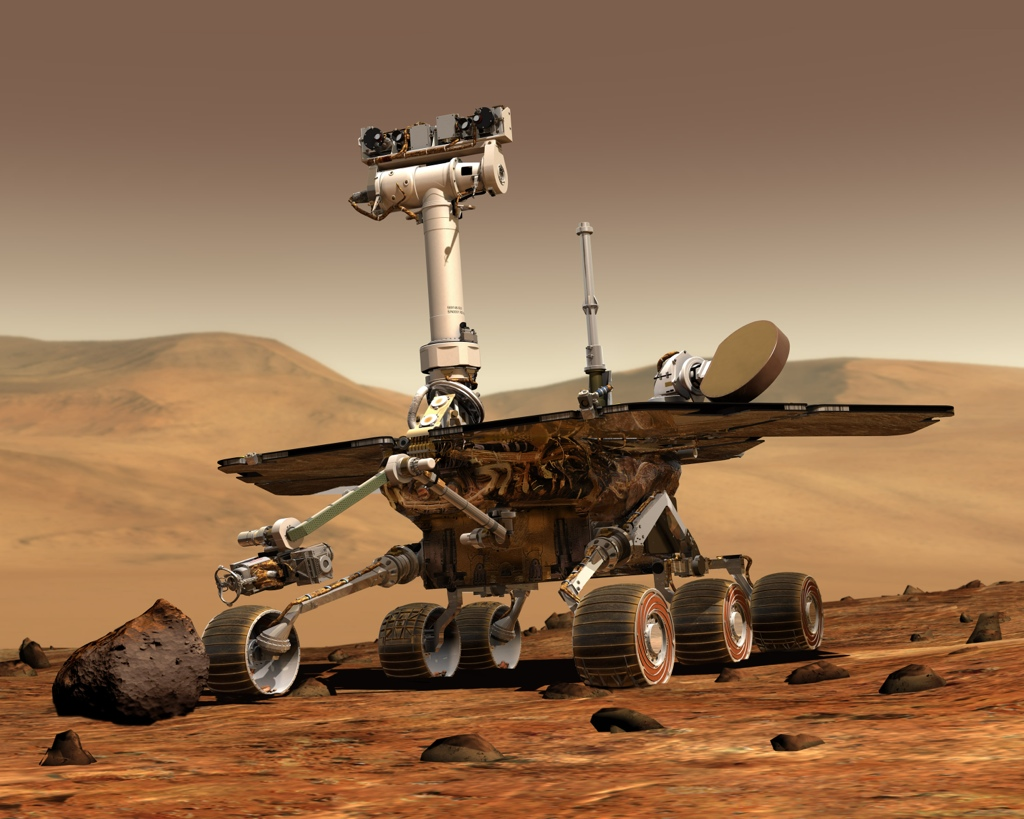
\includegraphics[width=6cm]{kapitel3/nasa_rover}
  \caption{Ein Nasa Rover}
  \label{Kap2:NasaRover}
\end{figure}

Man kann sich auch selbst ein Makro für das Einfügen von Bildern schreiben:

\bild{kapitel3/modell_point_to_point}{6cm}{Point to Point}

\begin{sidewaysfigure}
 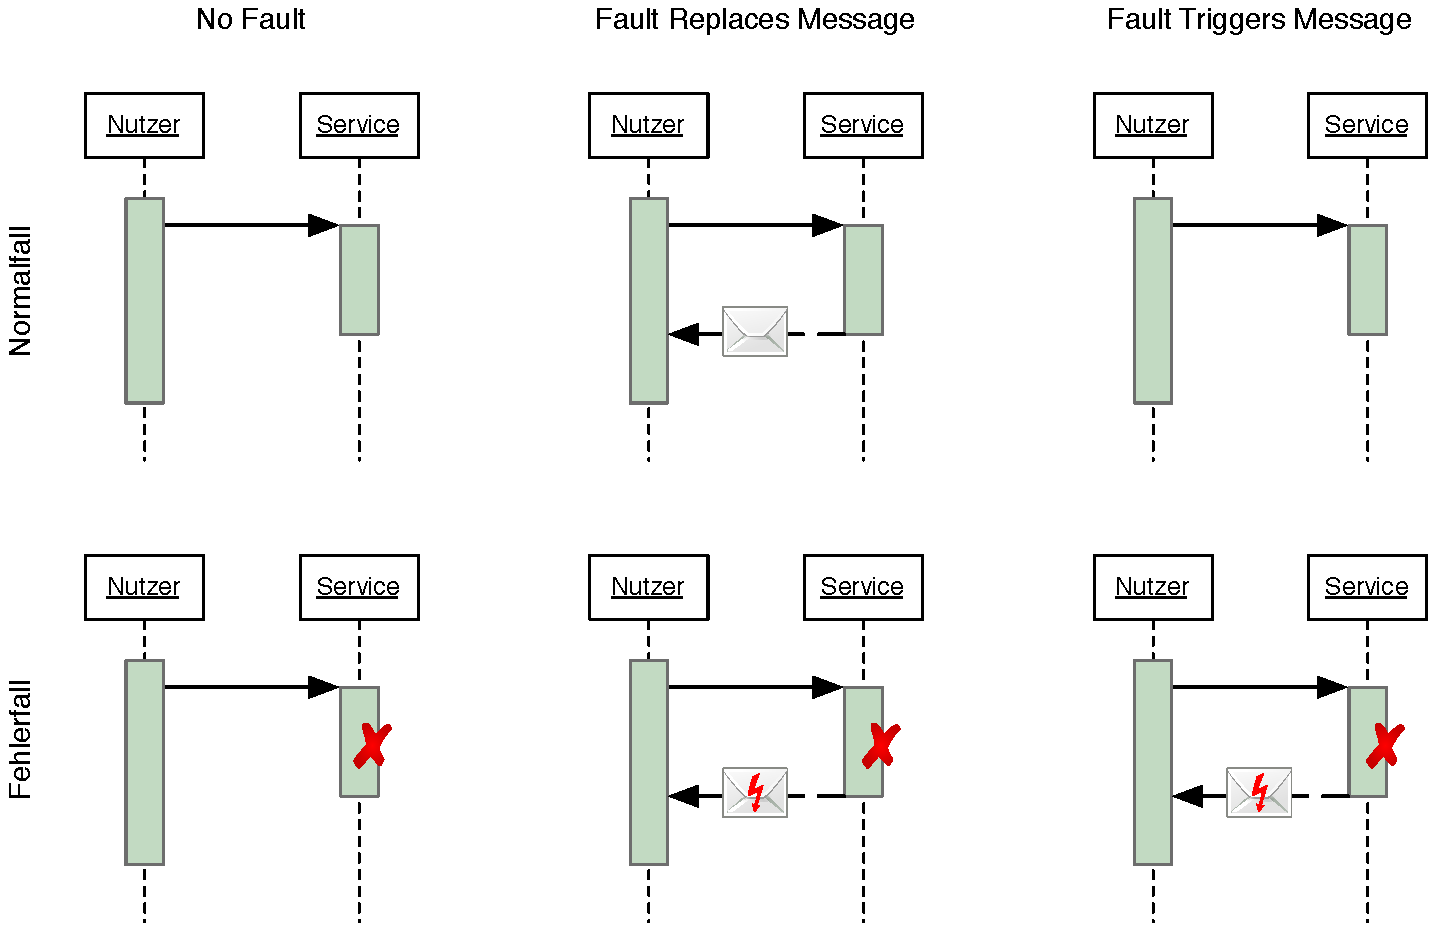
\includegraphics[width=22cm]{kapitel3/ws-wsdl20-fehler}
  \caption{Sehr große Grafiken kann man drehen, damit sie auf die Seite passen}
  \label{Kap2:wsdl-fehler}
\end{sidewaysfigure}

Möchte man verhindern, dass Bilder in ein anderes Kapitel rutschen, steht der Befehl \verb+\clearpage+ zur Verfügung, der \LaTeX{} zwingt, alle bis dahin definierten \textit{floats} (Bilder, Tabellen, Formeln etc.) auszugeben.

\clearpage % Alle Bilder, die bisher kamen ausgeben


\section{Formelsatz}

Eine Formel gefällig? Mitten im Text $a_2 = \sqrt{x^3}$ oder als eigener Absatz (siehe \autoref{Formel}):

\begin{equation}
\begin{bmatrix}
   1 &  4 &  2 \\
   4 &  0 & -3
\end{bmatrix}
        \cdot
\begin{bmatrix}
   1 &  1 &  0 \\
  -2 &  3 &  5 \\
   0 &  1 &  4
\end{bmatrix}
       {=}
\begin{bmatrix}
  -7 &  15 &  28 \\
   4 &   1 & -12
\end{bmatrix}
\label{Formel}
\end{equation}

Wenn Ihre Formel zu breit für eine Zeile wird, können Sie sie mithilfe der \texttt{split}-Umgebung und einem doppelten Backslash (\verb+\\+) umbrechen.

\begin{equation}
\label{eq:4}
\begin{split}
\mathbf{F}_{{eigen}}=\sqrt[3]{\coprod_{i=1}^{3} \lambda_{i}},
\frac{\lambda_{1}-\lambda_{3}}{\lambda_{1}},
\frac{\lambda_{2}-\lambda_{3}}{\lambda_{1}},
\frac{\lambda_{3}}{\lambda_{1}} \\-
\sum_{i=1}^{3} \lambda_{i} \log \left(\lambda_{i}\right),
\frac{\lambda_{1}-\lambda_{2}}{\lambda_{1}}
\end{split}
\end{equation}

Sie können Formelelemente auch am Gleichheitszeichen ausrichten, hierzu dient die \texttt{align}-Umgebung:

\begin{align}
2x - 5y &=  8 \\
3x + 92y &=  -12
\end{align}

Wollen Sie keine Nummerierung der Formeln, ergänzen Sie einfach einen \texttt{*} bei den Namen der Umgebungen, d.\,h. Sie verwenden \texttt{equation*} oder \texttt{align*}.

\begin{equation*}
\begin{bmatrix}
   1 &  4 &  2 \\
   4 &  0 & -3
\end{bmatrix}
        \cdot
\begin{bmatrix}
   1 &  1 &  0 \\
  -2 &  3 &  5 \\
   0 &  1 &  4
\end{bmatrix}
       {=}
\begin{bmatrix}
  -7 &  15 &  28 \\
   4 &   1 & -12
\end{bmatrix}
\end{equation*}

\section{Zahlendarstellung und Angabe von Einheiten}
Zahlen und Einheiten können wie folgt angegeben werden: 

\begin{tabular}{|l|l|}
	\hline
	\textbf{Befehl} & \textbf{Ausgabe}  \\\hline
	\verb*|\num{123}| & \num{123} \\
	\verb*|\num{1234}| &	\num{1234} \\
	\verb*|\num{12345}| &	\num{12345} \\
	\verb*|\num{0.123}| &	\num{0.123} \\
	\verb*|\num{0,12345}| &	\num{0,1234} \\
	\verb*|\num{.12345}| &	\num{.12345} \\
	\verb*|\num{3.45d-4}| &	\num{3.45d-4} \\
	\verb*|\num{-e10}| &	\num{-e10} \\
	\verb*|\qty[per-mode=symbol]{2.8}{\giga\byte\per\second}| & \qty[per-mode = symbol]{2.8}{\giga\byte\per\second}\\
	\verb*|\qty[per-mode=fraction]{2.8}{\giga\byte\per\second}| & \qty[per-mode = fraction]{2.8}{\giga\byte\per\second}\\
	\verb*|\qty[mode=text]{2.8}{\giga\byte\per\second}| & \qty[mode = text]{2.8}{\giga\byte\per\second}\\\hline
\end{tabular}

\vspace*{0.75cm}

Listen können ebenfalls mit Einheiten versehen werden:\\ \verb*|\qtylist{10;30;45}{\giga\byte\per\second}| liefert die Ausgabe: \qtylist{10;30;45}{\giga\byte\per\second}. 

Bereiche können mit dem Befehl \verb*|\qtyrange{10}{30}{\giga\byte\per\second}| ausgegeben werden. \qtyrange{10}{30}{\giga\byte\per\second}


\section{Sourcecode}

Man kann mit Latex auch ganz toll Sourcecode in den Text aufnehmen.

\subsection{Aus einer Datei}

\lstinputlisting[firstline=2,                 % Erste anzuzeigende Zeile aus der Datei
                 language=Java,               % Programmmiersprache (für Highlighting)
                 caption={Crypter-Interface}, % Beschriftung
                 label=lst:CrypterInterface]  % Label (für Referenzen)
                 {\srcloc/Crypter.java}       % Pfad zur Datei, die angezeigt wird

Mit Zeilennummern

\lstinputlisting[numbers=left,                % Mit Zeilennummern auf der linken Seite
                 firstline=10,                % Erste anzuzeigende Zeile aus der Datei
                 lastline=15,                 % Letzte anzuzeigende Zeile aus der Datei
                 language=Java,               % Programmmiersprache (für Highlighting)
                 caption={Crypter},           % Beschriftung
                 label=lst:CrypterInterface2] % Label (für Referenzen)
                 {\srcloc/Crypter.java}       % Pfad zur Datei, die angezeigt wird


\subsection{Inline}

\begin{lstlisting}[language=Java,caption=Methode checkKey()]
    /**
     * Testet den Schlüssel auf Korrektheit: Er muss mindestens die Länge 1
     * haben und darf nur Zeichen von A-Z enthalten.
     *
     * @param key zu testender Schlüssel
     * @throws CrypterException wenn der Schlüssel nicht OK ist.
     */
    protected void checkKey(Key key) throws CrypterException {

        // Passt die Länge?
        if (key.getKey().length == 0) {
            throw new CrypterException("Der Schlüssel muss mindestens " +
                    "ein Zeichen lang sein");
        }

        checkCharacters(key.getKey(), ALPHABET);
    }
\end{lstlisting}


\section{Anforderungen}

Anforderungen im Format des Volere"=Templates (Snowcards) \autocite{Volere} können per Makro eingefügt werden. Das Label wird automatisch mit der Nummer erstellt, d.\,h. Sie können auf die Tabelle mit dieser referenzieren (siehe \autoref{F52}).

\snowcard % Snowcard einbinden 
   {F52} % Nummer des Requirements
   {F} % Art
   {Hoch} % Priorität
   {User Authentifizierung} % Titel
   {Interview mit Abteilungsleiter} % Herkunft (Optional)
   {F12} % Konflikte (Optional)
   {Der Benutzer ist in der Lage sich über seinen
    Benutzernamen und sein Passwort am System anzumelden} % Beschreibung
   {Ein Benutzer kann sich mit seinem firmenweiten Benutzernamen und
   Passwort über die Anmeldemaske anmelden und hat Zugriff auf die
   Funktionen des Systems} % Fit-Kriterium (Optional)
   {Benutzerhandbuch des Altsystems} % Material (Optional)

Ebenso können Sie nicht"=funktionale Anforderungen mit Hilfe von Quality Attribute Scenarios (vgl. \autoref{NF11}) darstellen. Zu Details siehe \autocite{Barbacci2003}.

\qas % Quality-Attribute Scenario einbinden (Anpassungen in titelblatt.tex)
   {NF11} % Nummer des Requirements
   {Hoch} % Priotität
   {Performance des Jahresabschlusses} % Titel
   {Endbenutzer} % Quelle
   {Startet einen Jahresabschluss} % Stimulus
   {Buchhaltungssystem} % Artefakt
   {Das System befindet sich im normalen Betriebszustand} % Umgebung
   {Jahresabschluss ist durchgeführt und kann als PDF abgerufen werden} % Antwort
   {10 Minuten} % Antwort-Maß

Die Abgrenzung von funktionalen und nicht-funktionalen Anforderungen ist nicht immer einfach und bereitet manchen Studierenden Probleme. Als Hilfestellung kann die von der ISO25010 \autocite{ISO25010} zur Verfügung gestellte Liste dienen, siehe \autoref{kapitel3/iso25010}.

\bild{kapitel3/iso25010}{14cm}{Qualitätsmodell für Software-Produkte nach ISO25010}

\citeauthor{Bass2021} listen in \autocite{Bass2021} eine ähnliche Liste von Kategorien für nicht-funktionalen Anforderungen auf, die ebenfalls als Richtschnur dienen kann. Diese sind:

\begin{itemize}
  \item \textit{Verfügbarkeit} \textit{(availability)} -- umfasst Zuverlässigkeit (reliability), Robustheit (robustness), Fehlertoleranz (fault tolerance) und Skalierbarkeit (scalability)
  \item \textit{Anpassbarkeit} \textit{(modifiability)}, umfasst Wartbarkeit (maintainability), Verständlichkeit (understandability) und Portabilität (portability).
  \item \textit{Performanz} \textit{(performance)}
  \item \textit{Sicherheit} \textit{(security)}
  \item \textit{Testbarkeit} \textit{(testability)}
  \item \textit{Bedienbarkeit} \textit{(usability)}
\end{itemize}


\chapter{Track Changes - Manuelle Änderungsmarkierung}
In diesem Dokument können Track Changes \chreplaced[id=B1]{verwendet}{aktiviert und benutzt} werden\\ (\lstinline|\chreplaced[id=B1]{verwendet}{aktiviert und benutzt}|). Durch die ID können die Anmerkungen \chdeleted[id=B2]{einem} dem Autor zugeordnet werden (\verb|\chdeleted[id=B2]{einem}|). B1 steht für die erste betreuende Person und B2 für die zweite. Ergänzungen in einem Satz wie beispielsweise in diesem Satz \chadded[id=B1]{gibt es} kein Verb können über \lstinline|\chadded[id=B2]{gibt es}| hinzugefügt werden.  

Es ist ebenfalls möglich Textteile \chhighlight[id=B1]{hervorzuheben} mit dem Befehl \\ \lstinline|\chhighlight[id=B1]{hervorzuheben}|. Zudem können Kommentare\chcomment[id=B2]{das ist mein Kommentar} über den Befehl \lstinline|\chcomment[id=B2]{das ist mein Kommentar}| hinzugefügt werden.


Das Verzeichnis zur Ausgabe aller Änderungen erfolgt über das Flag \lstinline|tc| in der docinfo.tex.  Dieser Befehl ist vor der Abgabe unbedingt auf \lstinline|notc| zu ändern.

Weitere Informationen zu der Nutzung des Paketes finden Sie unter: \url{https://ctan.org/pkg/changes?lang=de}

\listofchanges[style=list, title=To Do's, show=all]







 % Externe Datei einbinden
%\chapter{Checkliste}
\label{Kap4}

Die folgende Checkliste kann dazu dienen, die Arbeit auf die wichtigsten Bewertungskriterien zu prüfen. Jeder Dozent hat andere Kriterien, die unten aufgeführten dürften aber für die meisten Dozenten gültig sein.

\section{Form und Sprache}

\begin{checklist}
  \footnotesize
  \item \textbf{Aufbau}: Die Arbeit ist nach wissenschaftlichen Prinzipien aufgebaut (wesentliche Teile vorhanden, Nummerierung/Verweise korrekt, Verzeichnisse vorhanden).
    \begin{checklist}
        \item \textit{Wesentliche Teile}: Die folgenden Elemente der Arbeit sind vorhanden: Titelblatt, Abstract/Zusammenfassung, Einleitung, Hauptteil, Fazit/Ausblick.
        \item \textit{Nummerierung/Verweise}: Das Nummerierungsschema wird konsistent über die gesamte Arbeit durchgehalten, die Verweise auf die verschiedenen Elemente (Abbildungen, Tabellen etc.) sind korrekt.
        \item \textit{Verzeichnisse}: Die Arbeit enthält alle relevanten Verzeichnisse: Inhaltsverzeichnis, Literaturverzeichnis, Abbildungsverzeichnis, Tabellenverzeichnis, eventuell Glossar.
    \end{checklist}
  \item \textbf{Sprache}: Die verwendete Sprache entspricht wissenschaftlichen Ansprüchen.
    \begin{checklist}
        \item \textit{Begriffe und Definitionen}: Begriffe werden einheitlich und konsistent verwendet. Neue Begriffe werden definiert und mit Literatur hinterlegt.
        \item \textit{Abkürzungen}: Alle Abkürzungen werden eingeführt und erläutert. Abkürzungen werden bei der ersten Verwendung ausgeschrieben und in einem Abkürzungsverzeichnis geführt. Es werden keine unüblichen oder selbst erfunden Abkürzungen verwendet. Ein Glossar kann verwendet werden, um Begriffe noch einmal kompakt darzustellen.
        \item \textit{Rechtschreibung}: Die Arbeit ist frei von Rechtschreibungs-, Zeichensetzungs- und Grammatikfehlern.
    \end{checklist}
  \item \textbf{Formatierung, Typografie}: Die Formatierung der Arbeit ist korrekt und aus typographischer Sicht einwandfrei. \textit{Wenn Sie dieses Template korrekt verwenden, sollte dieser Punkt automatisch durch die Verwendung von \LaTeX{} erledigt sein.}
    \begin{checklist}
        \item \textit{Korrekte Typografie}: Schriftarten werden korrekt verwendet (nicht mehr als 2 Fonts), der Zeilenabstand ist passend, die Ränder sind ausreichend, der Satz ist korrekt.
        \item \textit{Satz von Abbildungen, Tabellen etc.}: Abbildungen sind in der richtigen Auflösung dargestellt, die Tabellen sind korrekt gesetzt, mathematische Formeln und Symbole sind sauber dargestellt.
    \end{checklist}
  \item \textbf{Abbildungen}: Abbildungen werden in ausreichendem Umfang zur Förderung des Verständnisses eingesetzt. Sie werden korrekt im Text referenziert und sind, wo immer möglich, in einer Standardnotation erstellt.
    \begin{checklist}
        \item \textit{Ausreichende Verwendung}: Komplizierte Sachverhalte werden durch Abbildungen verdeutlicht. Es werden genug Abbildungen eingesetzt, um die wichtigsten Sachverhalte zu erklären.
        \item \textit{Verständnisförderung}: Abbildungen dienen nicht als Schmuck, sondern um komplizierte Sachverhalte zu verdeutlichen.
        \item \textit{Einbindung in den Text}: Der Text muss auch ohne Abbildungen verständlich sein, die Abbildungen helfen Sachverhalte aus dem Text besser darzustellen. Der Text referenziert die Abbildung korrekt.
        \item \textit{Standardnotation, Legende}: Die Abbildungen verwenden Standard"=Notationen wie UML, FMC etc. Wo keine Standardnotation eingesetzt wird, ist eine Legende vorhanden, um die Bildelemente zu erläutern.
    \end{checklist}
  \item \textbf{Zitate}: Quellen werden konsistent nach einer gängigen Zitierweise zitiert und sind vollständig im Literaturverzeichnis angegeben.
    \begin{checklist}
        \item \textit{Zitierweise}: Die Zitierweise in der gesamten Arbeit folgt einem einheitlichen Schema, \zb{} IEEE, DIN, Chicago.
        \item \textit{Vollständigkeit}: Alle Zitate sind als solche kenntlich gemacht und die Quelle wird vollständig angegeben, und Plagiate werden vermieden.
    \end{checklist}
  \item \textbf{Schreibstil}: Lebendiger, wissenschaftlicher und verständlicher Schreibstil.
    \begin{checklist}
        \item \textit{Wissenschaftlichkeit}: Der Text ist im Präsenz geschrieben, es wird die dritte Person verwendet, Fachausdrücke werden korrekt verwendet, Fremdwörter und Amerikanismen werden richtig eingesetzt.
        \item \textit{Verständlichkeit}: Abschweifungen und Wiederholungen werden vermieden, statt dessen werden präzise und übersichtliche Sätze verwendet.
        \item \textit{Lebendigkeit}: Der Text der Arbeit zeichnet sich durch eine gute Wortwahl, Sprachbilder, einen angemessenen Satzbau und eine hohe Variabilität aus.
    \end{checklist}
\end{checklist}

\section{Inhalt}

\begin{checklist}
  \footnotesize
  \item \textbf{Gliederung}: Die Gliederung ist vollständig, konsistent und sachlogisch mit angemessener Struktur und Tiefe.
    \begin{checklist}
        \item \textit{Konsistenz und Vollständigkeit}: Auf einer Ebene stehen keine Punkte alleine, die Gliederungspunkte orientieren sich an der Argumentationskette.
        \item \textit{Angemessene Tiefe}: Die Größe der einzelnen Unterpunkte ist vom Umfang her ähnlich. Es gibt keine Gliederungspunkte, die nur aus ein bis zwei Sätzen bestehen.
    \end{checklist}
  \item \textbf{Grundlagen}: Es werden alle relevanten Grundlagen gelegt. Der State"=of"=the"=art und der State"=of"=practice werden dargelegt.
    \begin{checklist}
        \item \textit{Umfang}: 1/3 des Hauptteils ist ein gutes Maß für eine ausreichende Darstellung der Grundlagen.
        \item \textit{Begriffe und Methoden}: Begriffe und Methoden sind definiert, und Literatur zu den Definitionen ist angegeben.
        \item \textit{State-of-the-art}: Der Stand des verfügbaren Wissens wird dargestellt, analysiert und kritisch beurteilt (state-of-the-art). Bei theoretischen Arbeiten kann ein eigenes Kapitel \enquote{verwandte Arbeiten} nötig sein, um den state"=of"=the"=art darzustellen.
        \item \textit{State-of-practice}: Bei praktischen Arbeiten, die in der Industrie geschrieben werden, kann es nötig sein, auch das Vorgehen im Unternehmen zu erläutern.
    \end{checklist}
  \item \textbf{Methodik/Lösung}: Die gewählte Methodik bzw. Lösung ist für das Problem adäquat.
    \begin{checklist}
        \item \textit{Anforderungen an die Lösung}: Die von der Lösung zu erfüllenden Anforderungen werden dargestellt. Wo nötig wird dies auf Grundlage eines sauberen Requirements"=Engineerings durchgeführt.
        \item \textit{Erläuterung des Lösungsansatzes}: Der gewählte Lösungsansatz wird ausführlich erläutert und verständlich dargestellt.
        \item \textit{Eignung zur Lösung der Aufgabe}: Die gewählte Lösung ist geeignet, um das beschriebene Problem zu lösen.
        \item \textit{Hypothesen}: Es sind ggf. Hypothesen gebildet worden; diese sind erläutert, und es sind Kriterien identifiziert worden, mit deren Hilfe man die Hypothesen falsifizieren kann.
        \item \textit{Alternativen}: Es werden Alternativen zur vorgeschlagenen Lösung diskutiert. Die eigene Lösung wird nicht als einzige mögliche dargestellt, sondern es werden auch andere mögliche Lösungen vorgestellt und bewertet.
        \item \textit{Begründung}: Alternativen und Kriterien für die Auswahl dieser Lösung werden dargestellt.
        \item \textit{Vorteile der Lösung}: Es wird dargestellt, wieso die entwickelte Lösung vorteilhafter ist als die bisherigen Ansätze. Diese Darstellung erfolgt auf Basis des Lösungsansatzes. Eine konkrete Validierung der Implementierung erfolgt ggf. in späteren Kapiteln.
    \end{checklist}
  \item \textbf{Logik der Argumentationskette}: Die Argumentation ist logisch und nachvollziehbar. Sie ist frei von logischen Fehlschlüssen.
  \item \textbf{Implementierung}: Wenn eine Implementierung der Lösung erfolgt, so wird die Implementierung beschrieben. Die Darstellung der Implementierung kann knapp ausfallen. Wichtig ist der Lösungsansatz, nicht die konkrete Umsetzung.
  \item \textbf{Validierung}: Die vorgeschlagene Lösung wird ggf. empirisch verprobt.
    \begin{checklist}
        \item \textit{Vorgehensweise}: Die Vorgehensweise zur Validierung der Lösung / Hypothesen ist beschrieben und geeignet, relevante Aspekte der Lösung zu überprüfen.
        \item \textit{Empirische Analyse}: Die Erfassungsmethode wird dargestellt und die Daten werden nach den Grundsätzen ordnungsgemäßer Laborpraxis gesammelt und statistisch korrekt ausgewertet.
        \item \textit{Verprobung}: Die Lösung wird an einem praktischen Beispiel verprobt, und es werden wissenschaftlich korrekte Schlüsse aus der Anwendung gezogen.
        \item \textit{Zielerreichung}: Funktioniert die gewählte Lösung nach der Implementierung? Wie weit wurde das Ziel erreicht? Falls nicht, gibt es nachvollziehbare Gründe dafür und wurden diese dargestellt?
    \end{checklist}
  \item \textbf{Diskussion}: Die Lösung und ihre Validierung wird kritisch und im Kontext möglicher Alternativen diskutiert und bewertet.
    \begin{checklist}
        \item \textit{Kritische Reflexion}: Grenzen und Schwächen der eigenen Ergebnisse werden beleuchtet.
        \item \textit{Ableitung von Konsequenzen}: Die Konsequenzen aus den Ergebnissen für die Wissenschaft und Praxis sind beschrieben.
    \end{checklist}
  \item \textbf{Quellenarbeit}: Es werden hochwertige Quellen in ausreichendem Umfang genutzt und kritisch hinterfragt. Eventuell vorhandene Quellen aus dem Unternehmen werden ebenfalls berücksichtigt.
    \begin{checklist}
        \item \textit{Umfang}: Der Umfang an Quellen richtet sich stark nach Thema und Art der Arbeit. Bei einer Bachelorarbeit sind mindestens 20--30 Quellen üblich, bei einer Masterarbeit deutlich mehr.
        \item \textit{Wissenschaftliche Qualität}: Nicht zitierfähig sind Internet"=Quellen, Wikipedia"=Einträge sowie andere Bachelor- oder Masterarbeiten (sofern nicht veröffentlicht). Das ausschließliche Zitieren von Lehrbüchern ist problematisch. Aktuelle wissenschaftliche Artikel und Werke sollten in den Quellen auftauchen.
        \item \textit{Quellen \enquote{aus der Praxis}}: Wenn es im Unternehmen spezielle Quellen und Informationen gibt, so werden diese berücksichtigt, z. B. firmen- oder branchenspezifischer Informationen.
        \item \textit{Kritische Würdigung}: Quellen und Zitate werden kritisch hinterfragt und nicht einfach unreflektiert übernommen. Es gibt eine kritische Distanz bei der Quellenauswahl und Quellenauswertung.
    \end{checklist}
  \item \textbf{Fazit}: Es wird eine Zusammenfassung der Arbeit sowie Ausblick auf weitere mögliche Arbeiten im Themenfeld gegeben, etwa die Lösung ausstehender Probleme oder die Erfüllung zusätzlicher Anforderungen.
  \item \textbf{Umfang der Arbeit}: Richtgrößen: Bachelorarbeiten: 50--80 Seiten, Masterarbeiten: 60--100 Seiten, jeweils ohne Verzeichnisse und Anhang.
\end{checklist}

\section{Vor der Abgabe}

\begin{checklist}
  \footnotesize
  \item \textit{Korrektur}: Haben Sie einen Dritten die Arbeit lesen lassen und alle gefundenen Rechtschreib- und Zeichensetzungsfehler behoben?
  \item \textit{Literaturverzeichnis}: Sind im Literaturverzeichnis irrelevante Informationen entfernt? Beispielsweise bei Büchern unnötige Informationen über die Herkunft bei Google-Books oder bei Papern doppelte Angaben der DOI?
  \item \textbf{Abgabe auf Papier}
  \begin{checklist}
    \item \textit{Template passend eingestellt}: Haben Sie in der Datei \texttt{thesis.tex} eingestellt, dass Sie auf Papier abgeben wollen?
    \item \textit{Doppel- oder einseitiger Druck}: Entspricht die Einstellung des Templates dem Druck, d.\,h. ist das Template für doppelseitigen Druck eingestellt, wenn doppelseitig gedruckt werden soll und umgekehrt?
    \item \textit{Umschläge}: Sind die Umschläge vorhanden, um die Arbeit später zu binden? Die Umschläge können in der Hausdruckerei der Technischen Hochschule erworben werden.
    \item \textit{Copyshop}: Wissen Sie, wo Sie die Arbeit drucken werden? Die Hausdruckerei kann Ihre Arbeit nicht drucken.
    \item \textit{Exemplare}: Haben Sie geklärt, ob der Zweitkorrektor auch ein gedrucktes Exemplar möchte?
  \end{checklist}
  \item \textbf{Digitale Abgabe}
  \begin{checklist}
    \item \textit{Zustimmung des Betreuers/der Betreuerin}: Haben Sie mit Ihrer Betreuerin bzw. Ihrem Betreuer abgeklärt, dass Sie digital abgeben dürfen?
    \item \textit{Template passend eingestellt}: Haben Sie in der Datei \texttt{thesis.tex} eingestellt, dass Sie digital abgeben wollen?
    \item \textit{Unterschrift}: Haben Sie Ihre Unterschrift eingescannt und unter dem Namen \texttt{unterschrift.png} im Hauptverzeichnis abgelegt?
  \end{checklist}
\end{checklist}
 % Externe Datei einbinden



\label{lastpage}
%Beginn des Anhangs. Befehl \appendix nicht entfernen, auch wenn kein Anhang vorhanden ist!
\appendix

%Wenn Sie keinen Anhang haben, entfernen Sie ausschließlich die nachfolgenden beiden Dateien.
\chapter{Anhang}\label{ch:anhang}

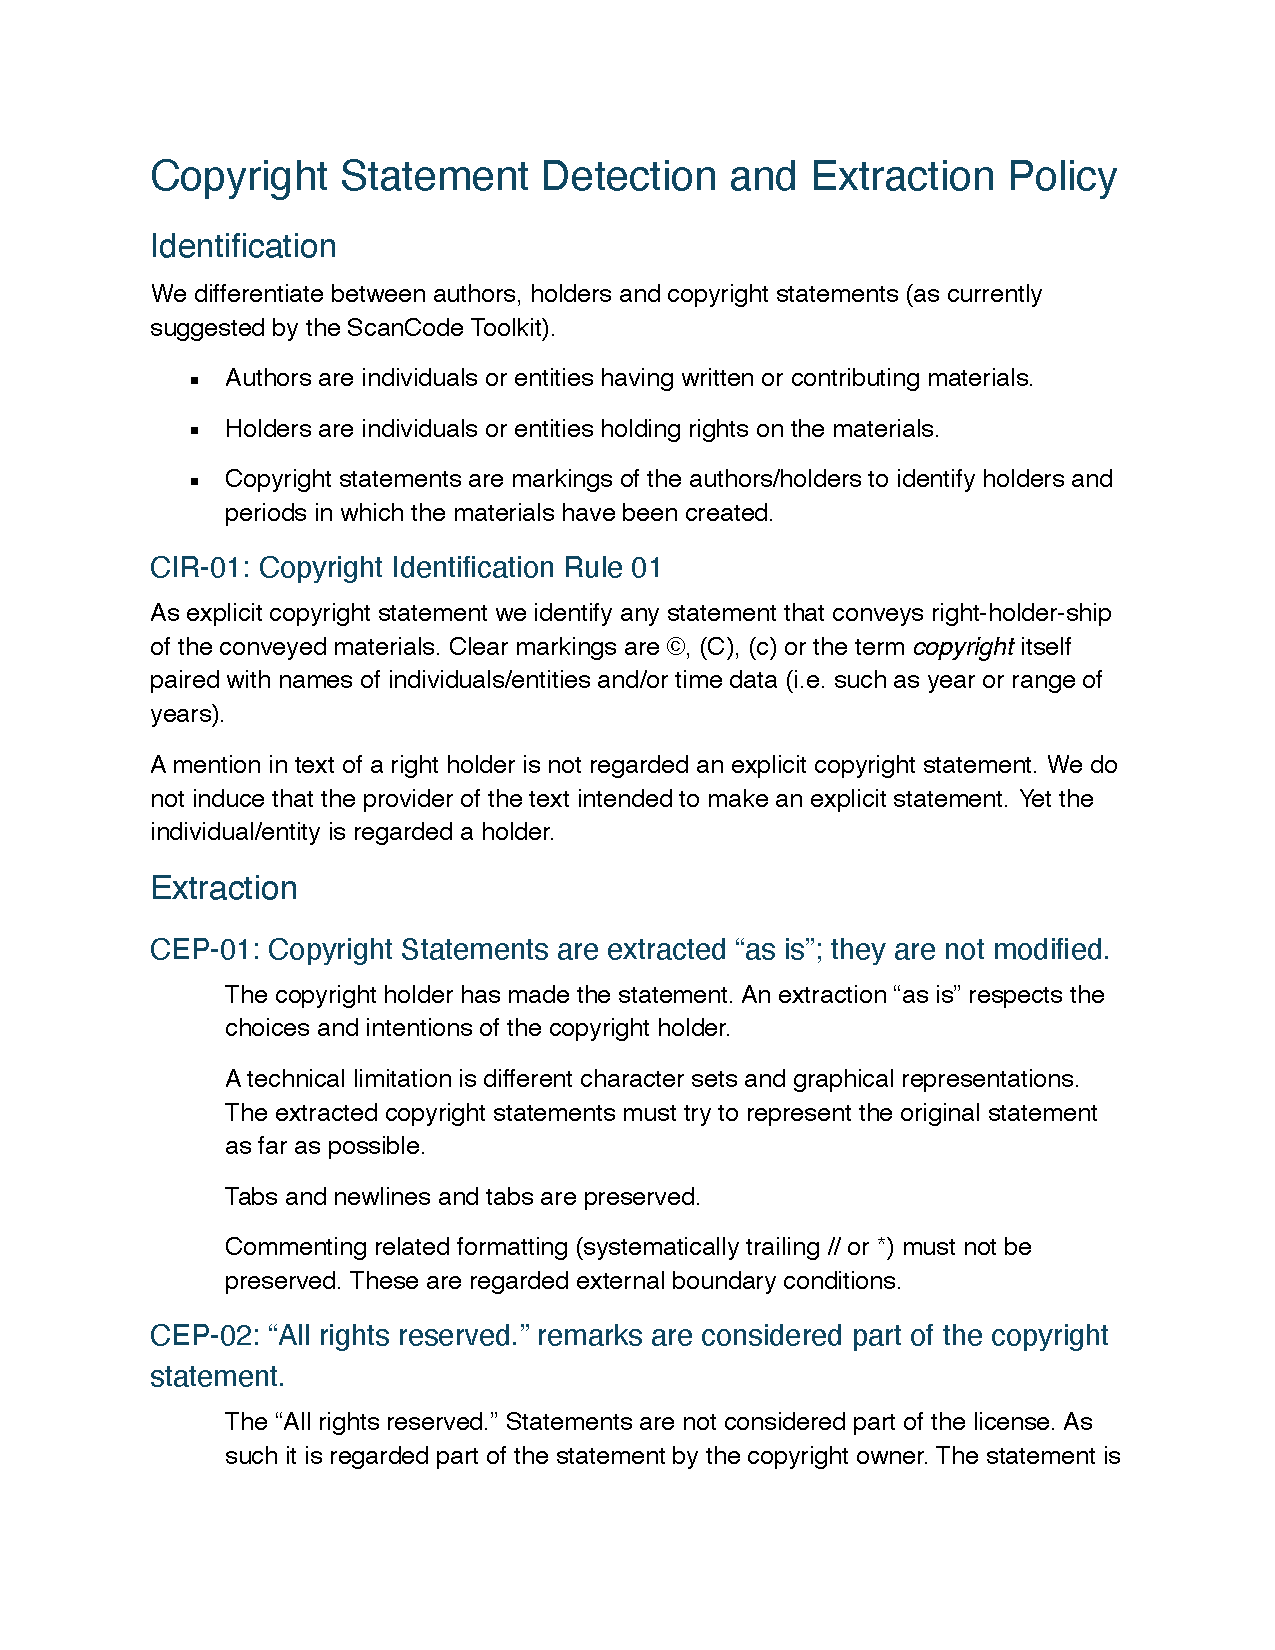
\includepdf[pages=-        % Alle Seiten des Dokumentes einbinden
,scale=.8      % Seiten verkleinern, damit sie zum Layout passen
,pagecommand={} % Layout des umgebenden Dokumentes belassen
]{pdfs/2025-03-28-Copyright Statement Detection and Extraction Policy}
%\chapter{Zweiter Anhang: Lange Tabelle}
\label{AnhangB}

Hier ein Beispiel für einen Anhang. Der Anhang kann genauso in Kapitel und Unterkapitel unterteilt werden, wie die anderen Teile der Arbeit auch.

\sffamily
\begin{footnotesize}
  \begin{longtable}[c]{ p{.5\textwidth} p{.1\textwidth} p{.1\textwidth} p{.1\textwidth}}
    \caption[Tabelle mit ISO-Ländercodes]                       % Caption für das Tabellenverzeichnis
        {Lange Tabelle mit ISO-Ländercodes\label{laendercodes}} % Caption für die Tabelle selbst
        \\
    \toprule
    \textbf{Country} & \textbf{A 2} & \textbf{A 3} & \textbf{Number} \\
    \midrule
    AFGHANISTAN                                    & AF & AFG & 004 \\
    ALBANIA                                        & AL & ALB & 008 \\
    ALGERIA                                        & DZ & DZA & 012 \\
    AMERICAN SAMOA                                 & AS & ASM & 016 \\
    ANDORRA                                        & AD & AND & 020 \\
    ANGOLA                                         & AO & AGO & 024 \\
    ANGUILLA                                       & AI & AIA & 660 \\
    ANTARCTICA                                     & AQ & ATA & 010 \\
    ANTIGUA AND BARBUDA                            & AG & ATG & 028 \\
    ARGENTINA                                      & AR & ARG & 032 \\
    ARMENIA                                        & AM & ARM & 051 \\
    ARUBA                                          & AW & ABW & 533 \\
    AUSTRALIA                                      & AU & AUS & 036 \\
    AUSTRIA                                        & AT & AUT & 040 \\
    AZERBAIJAN                                     & AZ & AZE & 031 \\
    BAHAMAS                                        & BS & BHS & 044 \\
    BAHRAIN                                        & BH & BHR & 048 \\
    BANGLADESH                                     & BD & BGD & 050 \\
    BARBADOS                                       & BB & BRB & 052 \\
    BELARUS                                        & BY & BLR & 112 \\
    BELGIUM                                        & BE & BEL & 056 \\
    BELIZE                                         & BZ & BLZ & 084 \\
    BENIN                                          & BJ & BEN & 204 \\
    BERMUDA                                        & BM & BMU & 060 \\
    BHUTAN                                         & BT & BTN & 064 \\
    BOLIVIA                                        & BO & BOL & 068 \\
    BOSNIA AND HERZEGOWINA                         & BA & BIH & 070 \\
    BOTSWANA                                       & BW & BWA & 072 \\
    BOUVET ISLAND                                  & BV & BVT & 074 \\
    BRAZIL                                         & BR & BRA & 076 \\
    BRITISH INDIAN OCEAN TERRITORY                 & IO & IOT & 086 \\
    BRUNEI DARUSSALAM                              & BN & BRN & 096 \\
    BULGARIA                                       & BG & BGR & 100 \\
    BURKINA FASO                                   & BF & BFA & 854 \\
    BURUNDI                                        & BI & BDI & 108 \\
    CAMBODIA                                       & KH & KHM & 116 \\
    CAMEROON                                       & CM & CMR & 120 \\
    CANADA                                         & CA & CAN & 124 \\
    CAPE VERDE                                     & CV & CPV & 132 \\
    CAYMAN ISLANDS                                 & KY & CYM & 136 \\
    CENTRAL AFRICAN REPUBLIC                       & CF & CAF & 140 \\
    CHAD                                           & TD & TCD & 148 \\
    CHILE                                          & CL & CHL & 152 \\
    CHINA                                          & CN & CHN & 156 \\
    CHRISTMAS ISLAND                               & CX & CXR & 162 \\
    COCOS (KEELING) ISLANDS                        & CC & CCK & 166 \\
    COLOMBIA                                       & CO & COL & 170 \\
    COMOROS                                        & KM & COM & 174 \\
    CONGO                                          & CG & COG & 178 \\
    COOK ISLANDS                                   & CK & COK & 184 \\
    COSTA RICA                                     & CR & CRI & 188 \\
    COTE D'IVOIRE                                  & CI & CIV & 384 \\
    CROATIA (local name: Hrvatska)                 & HR & HRV & 191 \\
    CUBA                                           & CU & CUB & 192 \\
    CYPRUS                                         & CY & CYP & 196 \\
    CZECH REPUBLIC                                 & CZ & CZE & 203 \\
    DENMARK                                        & DK & DNK & 208 \\
    DJIBOUTI                                       & DJ & DJI & 262 \\
    DOMINICA                                       & DM & DMA & 212 \\
    DOMINICAN REPUBLIC                             & DO & DOM & 214 \\
    EAST TIMOR                                     & TP & TMP & 626 \\
    ECUADOR                                        & EC & ECU & 218 \\
    EGYPT                                          & EG & EGY & 818 \\
    EL SALVADOR                                    & SV & SLV & 222 \\
    EQUATORIAL GUINEA                              & GQ & GNQ & 226 \\
    ERITREA                                        & ER & ERI & 232 \\
    ESTONIA                                        & EE & EST & 233 \\
    ETHIOPIA                                       & ET & ETH & 210 \\
    FALKLAND ISLANDS (MALVINAS)                    & FK & FLK & 238 \\
    FAROE ISLANDS                                  & FO & FRO & 234 \\
    FIJI                                           & FJ & FJI & 242 \\
    \bottomrule
  \end{longtable}
\end{footnotesize}
\rmfamily


\textit{Beachten Sie, dass die Tabelle manchmal erst nach dreimaligem Lauf durch \LaTeX{} richtig angezeigt wird.}



\end{document}

